\PassOptionsToPackage{unicode=true}{hyperref} % options for packages loaded elsewhere
\PassOptionsToPackage{hyphens}{url}
\PassOptionsToPackage{dvipsnames,svgnames*,x11names*}{xcolor}
%
\documentclass[
]{article}
\usepackage{lmodern}
\usepackage{amssymb,amsmath}
\usepackage{ifxetex,ifluatex}
\ifnum 0\ifxetex 1\fi\ifluatex 1\fi=0 % if pdftex
  \usepackage[T1]{fontenc}
  \usepackage[utf8]{inputenc}
  \usepackage{textcomp} % provides euro and other symbols
\else % if luatex or xelatex
  \usepackage{unicode-math}
  \defaultfontfeatures{Scale=MatchLowercase}
  \defaultfontfeatures[\rmfamily]{Ligatures=TeX,Scale=1}
\fi
% use upquote if available, for straight quotes in verbatim environments
\IfFileExists{upquote.sty}{\usepackage{upquote}}{}
\IfFileExists{microtype.sty}{% use microtype if available
  \usepackage[]{microtype}
  \UseMicrotypeSet[protrusion]{basicmath} % disable protrusion for tt fonts
}{}
\makeatletter
\@ifundefined{KOMAClassName}{% if non-KOMA class
  \IfFileExists{parskip.sty}{%
    \usepackage{parskip}
  }{% else
    \setlength{\parindent}{0pt}
    \setlength{\parskip}{6pt plus 2pt minus 1pt}}
}{% if KOMA class
  \KOMAoptions{parskip=half}}
\makeatother
\usepackage{xcolor}
\IfFileExists{xurl.sty}{\usepackage{xurl}}{} % add URL line breaks if available
\IfFileExists{bookmark.sty}{\usepackage{bookmark}}{\usepackage{hyperref}}
\hypersetup{
  pdftitle={PERSUADE BC\_OS\_output},
  colorlinks=true,
  linkcolor=Maroon,
  filecolor=Maroon,
  citecolor=Blue,
  urlcolor=blue,
  breaklinks=true}
\urlstyle{same}  % don't use monospace font for urls
\usepackage[margin=1in]{geometry}
\usepackage{graphicx,grffile}
\makeatletter
\def\maxwidth{\ifdim\Gin@nat@width>\linewidth\linewidth\else\Gin@nat@width\fi}
\def\maxheight{\ifdim\Gin@nat@height>\textheight\textheight\else\Gin@nat@height\fi}
\makeatother
% Scale images if necessary, so that they will not overflow the page
% margins by default, and it is still possible to overwrite the defaults
% using explicit options in \includegraphics[width, height, ...]{}
\setkeys{Gin}{width=\maxwidth,height=\maxheight,keepaspectratio}
\setlength{\emergencystretch}{3em}  % prevent overfull lines
\providecommand{\tightlist}{%
  \setlength{\itemsep}{0pt}\setlength{\parskip}{0pt}}
\setcounter{secnumdepth}{-2}
% Redefines (sub)paragraphs to behave more like sections
\ifx\paragraph\undefined\else
  \let\oldparagraph\paragraph
  \renewcommand{\paragraph}[1]{\oldparagraph{#1}\mbox{}}
\fi
\ifx\subparagraph\undefined\else
  \let\oldsubparagraph\subparagraph
  \renewcommand{\subparagraph}[1]{\oldsubparagraph{#1}\mbox{}}
\fi

% set default figure placement to htbp
\makeatletter
\def\fps@figure{htbp}
\makeatother

\usepackage{booktabs}
\usepackage{longtable}
\usepackage{array}
\usepackage{multirow}
\usepackage{wrapfig}
\usepackage{float}
\usepackage{colortbl}
\usepackage{pdflscape}
\usepackage{tabu}
\usepackage{threeparttable}
\usepackage{threeparttablex}
\usepackage[normalem]{ulem}
\usepackage{makecell}
\usepackage{xcolor}

\title{PERSUADE BC\_OS\_output}
\author{}
\date{\vspace{-2.5em}2021-02-11}

\begin{document}
\maketitle

{
\hypersetup{linkcolor=}
\setcounter{tocdepth}{2}
\tableofcontents
}
~\\

\href{https://github.com/Bram-R/PERSUADE}{Link to PERSUADE GitHub page}
\newpage

\hypertarget{kaplan-meier}{%
\section{Kaplan-Meier}\label{kaplan-meier}}

\begin{flushleft}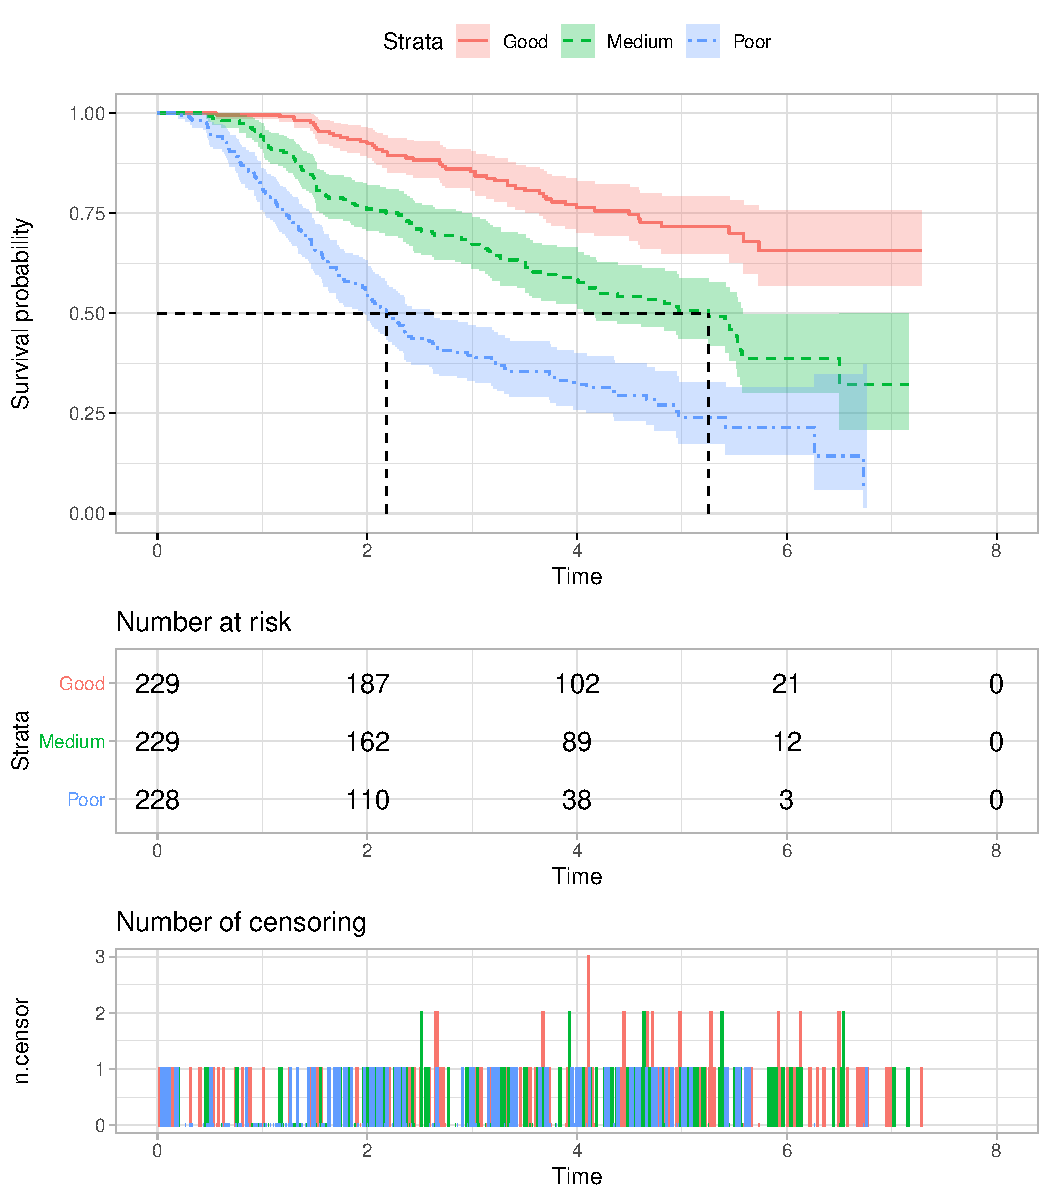
\includegraphics{Images/plot_KM-1} \end{flushleft}

\begin{table}[H]
\centering
\begin{tabular}{lrrrrrrrrr}
\toprule
  & records & n.max & n.start & events & *rmean & *se(rmean) & median & 0.95LCL & 0.95UCL\\
\midrule
\cellcolor{gray!6}{group=Good} & \cellcolor{gray!6}{229} & \cellcolor{gray!6}{229} & \cellcolor{gray!6}{229} & \cellcolor{gray!6}{51} & \cellcolor{gray!6}{5.934330} & \cellcolor{gray!6}{0.1616003} & \cellcolor{gray!6}{NA} & \cellcolor{gray!6}{NA} & \cellcolor{gray!6}{NA}\\
group=Medium & 229 & 229 & 229 & 103 & 4.600852 & 0.1856699 & 5.254795 & 4.115068 & 5.572603\\
\cellcolor{gray!6}{group=Poor} & \cellcolor{gray!6}{228} & \cellcolor{gray!6}{228} & \cellcolor{gray!6}{228} & \cellcolor{gray!6}{145} & \cellcolor{gray!6}{3.101736} & \cellcolor{gray!6}{0.1772520} & \cellcolor{gray!6}{2.183562} & \cellcolor{gray!6}{1.978082} & \cellcolor{gray!6}{2.619178}\\
\bottomrule
\end{tabular}
\end{table}

\newpage

\hypertarget{stratified-models}{%
\section{Stratified models?}\label{stratified-models}}

\hypertarget{should-stratified-parametric-survival-models-be-used}{%
\subsection{Should stratified parametric survival models be
used?}\label{should-stratified-parametric-survival-models-be-used}}

To inform the decision whether stratified or non-stratified models
should be used. One should assess whether the proportional hazard (PH)
assumption holds. The PH assumption entails that the ratio of the
hazards of two groups is constant over time. When the PH assumption
holds, one may fit non-stratified (parametric) survival models, meaning
that a single (parametric) survival model can be fitted to all groups
with the group effect(s) included as a covariate of the model. When the
PH assumption does not hold it is advised to fit separate (parametric)
survival models to the different groups. Finally, proportional hazards
is only relevant for exponential, Weibull, and Gompertz models.
Log-logistic and log normal models since these are accelerated failure
time models and, by definition, do not consider hazards to be
proportional over time. Group (treatment) effect can of course be
modelled as a covariate when using these models. For more information,
please refer to the
\href{http://nicedsu.org.uk/wp-content/uploads/2016/03/NICE-DSU-TSD-Survival-analysis.updated-March-2013.v2.pdf}{NICE
TSD 14}.\\
The figures below allow to examine whether the PH assumption holds.
Figure A shows the relation between the natural logarithm of time
(x-axis) and the natural logarithm of the cumulative hazard (y-axis).
The lines in the figure representing the different groups. An indication
that the PH assumption holds is when these lines are parallel. Figures B
and C represent the scaled Schoenfeld residual plots. In those plots,
the relation of time (x-axis) and the residuals of each observed events
(y-axis) is plotted. For the PH assumption to hold, there should be not
apparent relations between these residuals and time. To investigate
this, a smoothed spline has been plotted (cyan). Once this smoothed line
systematically deviates from a straight line with intercept 0, one can
consider that the PH assumption is violated, because it indicates a
relation between the coefficient (or group variable in this case) and
time. This is demonstrated in
\href{https://doi.org/10.1093/biomet/81.3.515}{the paper from Grambsch
and Therneau, Biometrika, Volume 81, Issue 3, September 1994, Pages
515--526}.\\
Another indication that the PH assumption does not hold is when the
lines from different groups Kaplan-Meier plot (previous page) cross each
other.\\
\textbf{Interpretation in this case}: Based on Figure A, one could argue
that the PH assumption holds since the different lines look quite
parallel to each other. However, when inspecting Figures B and C, one
can see that the hazard first decreases and then increases over time (in
both Figures). This indicates that the PH assumption probably does not
hold.\\
\textbf{CAUTION}: An indication that the PH assumption holds during the
observed period of time does not indicate that it holds after the
observation period (during the extrapolation).

\begin{flushleft}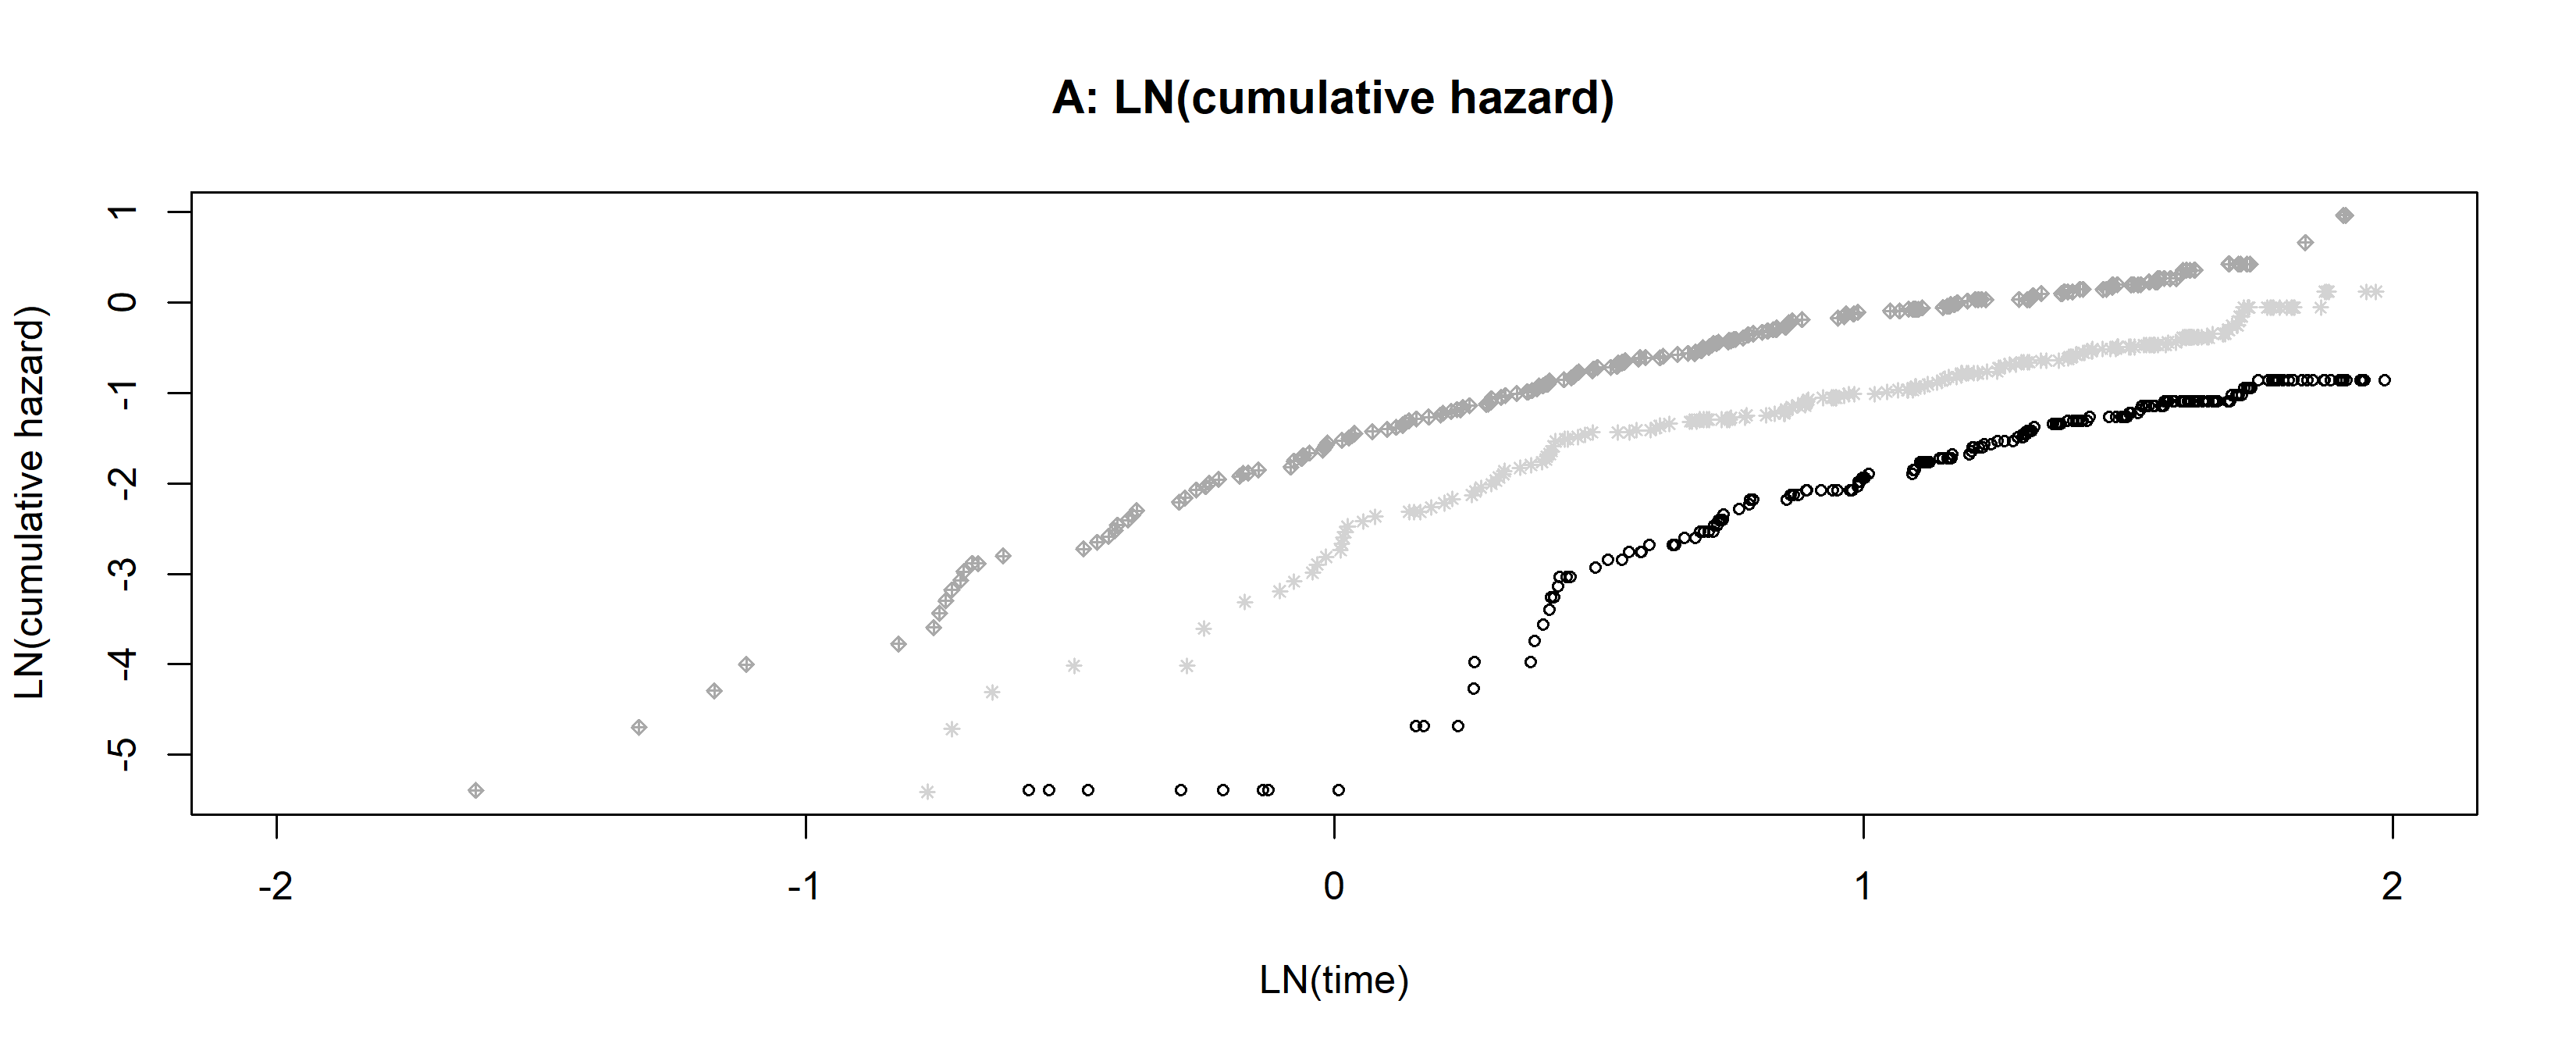
\includegraphics[height=0.29\textheight]{Images/PH_assumption-1} \end{flushleft}

\begin{flushleft}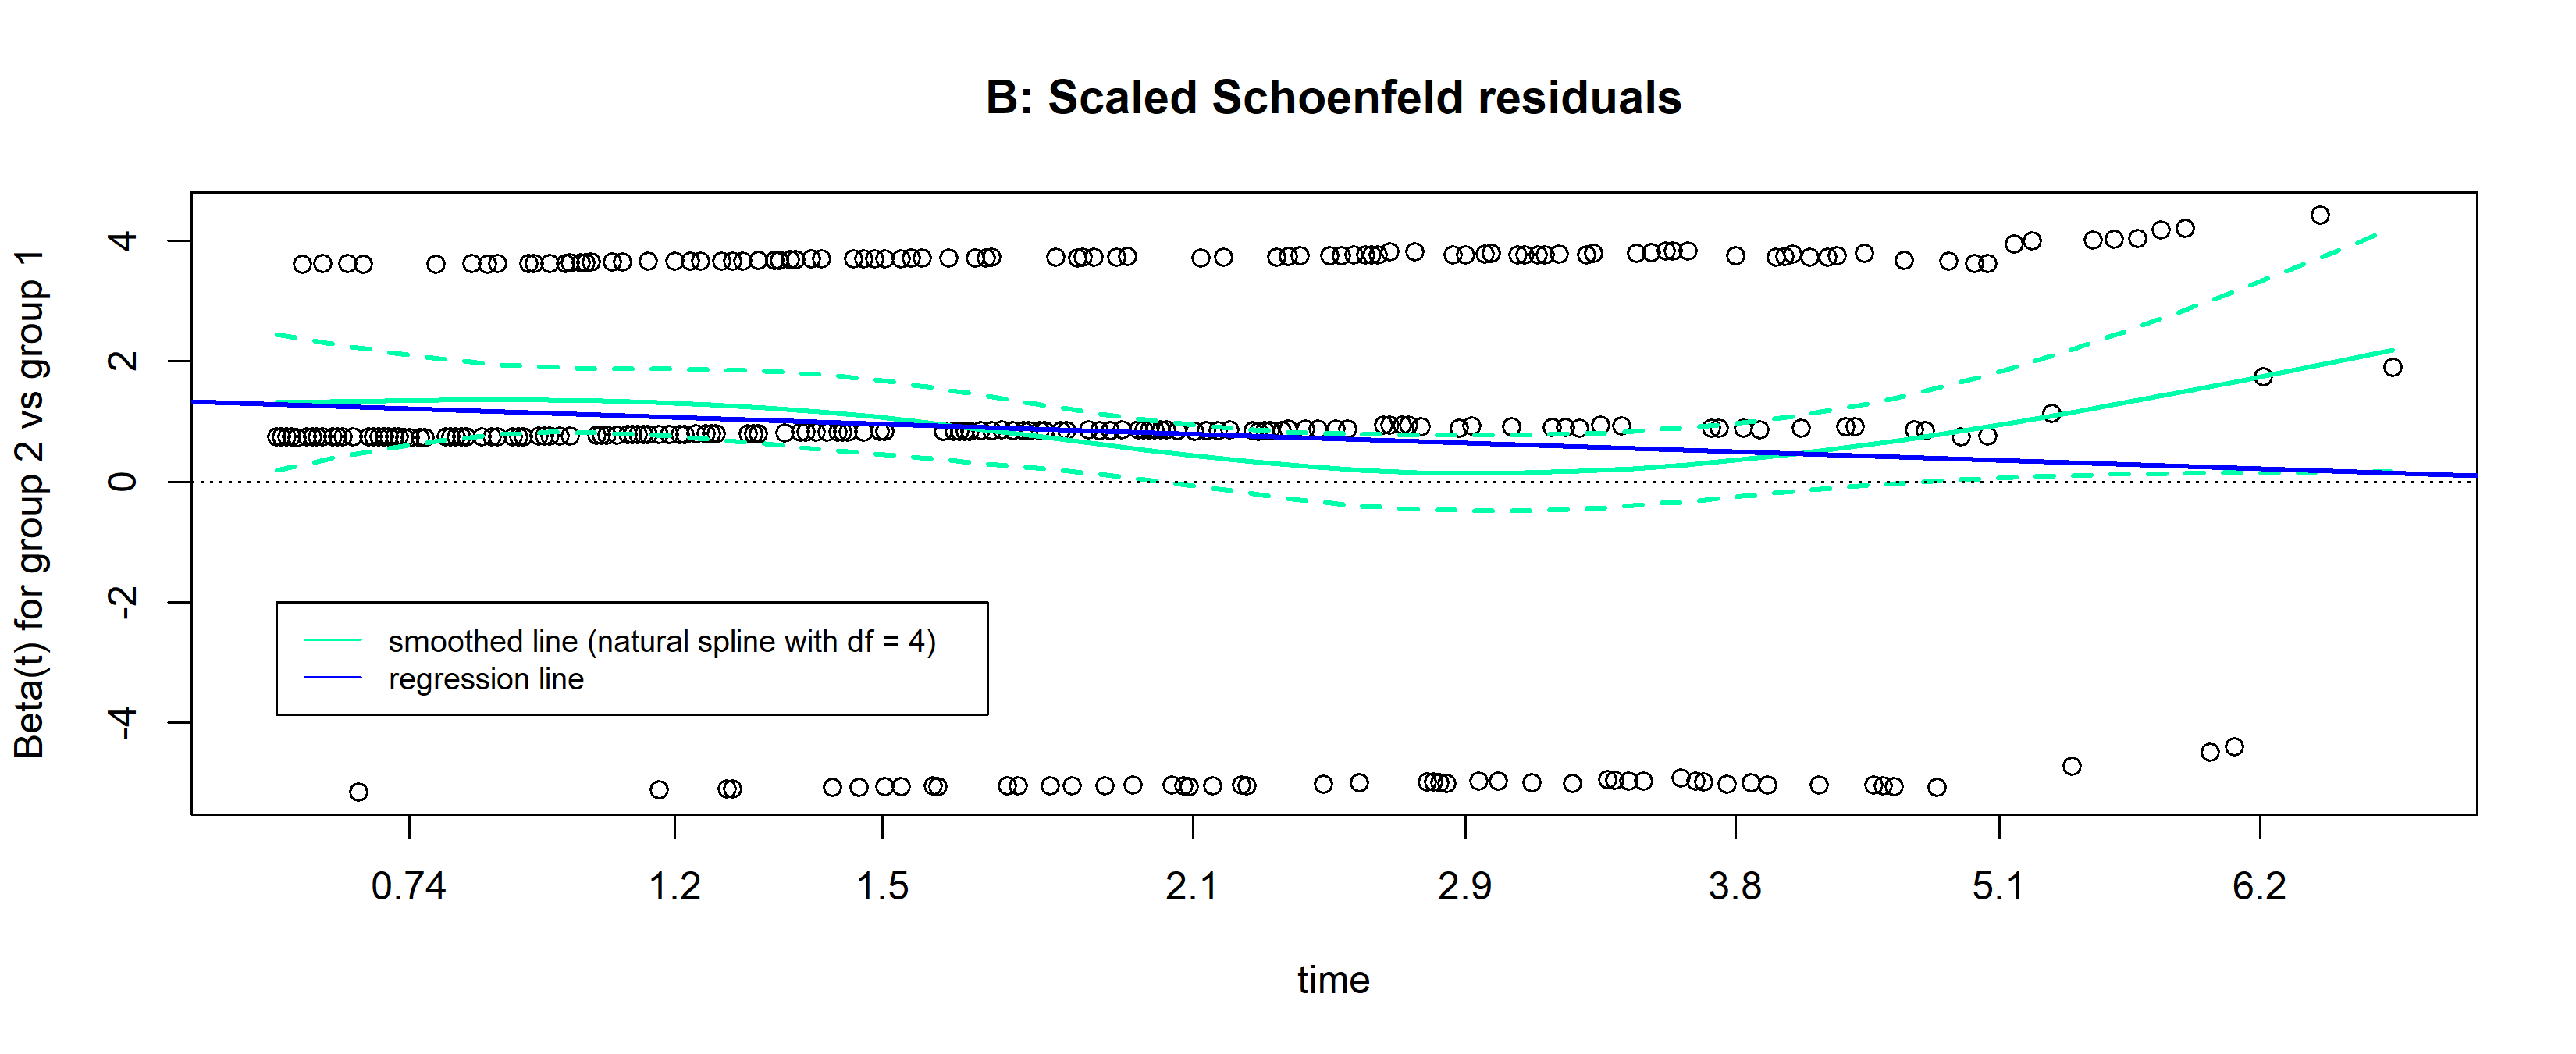
\includegraphics[height=0.29\textheight]{Images/PH_assumption-2} \end{flushleft}

\begin{flushleft}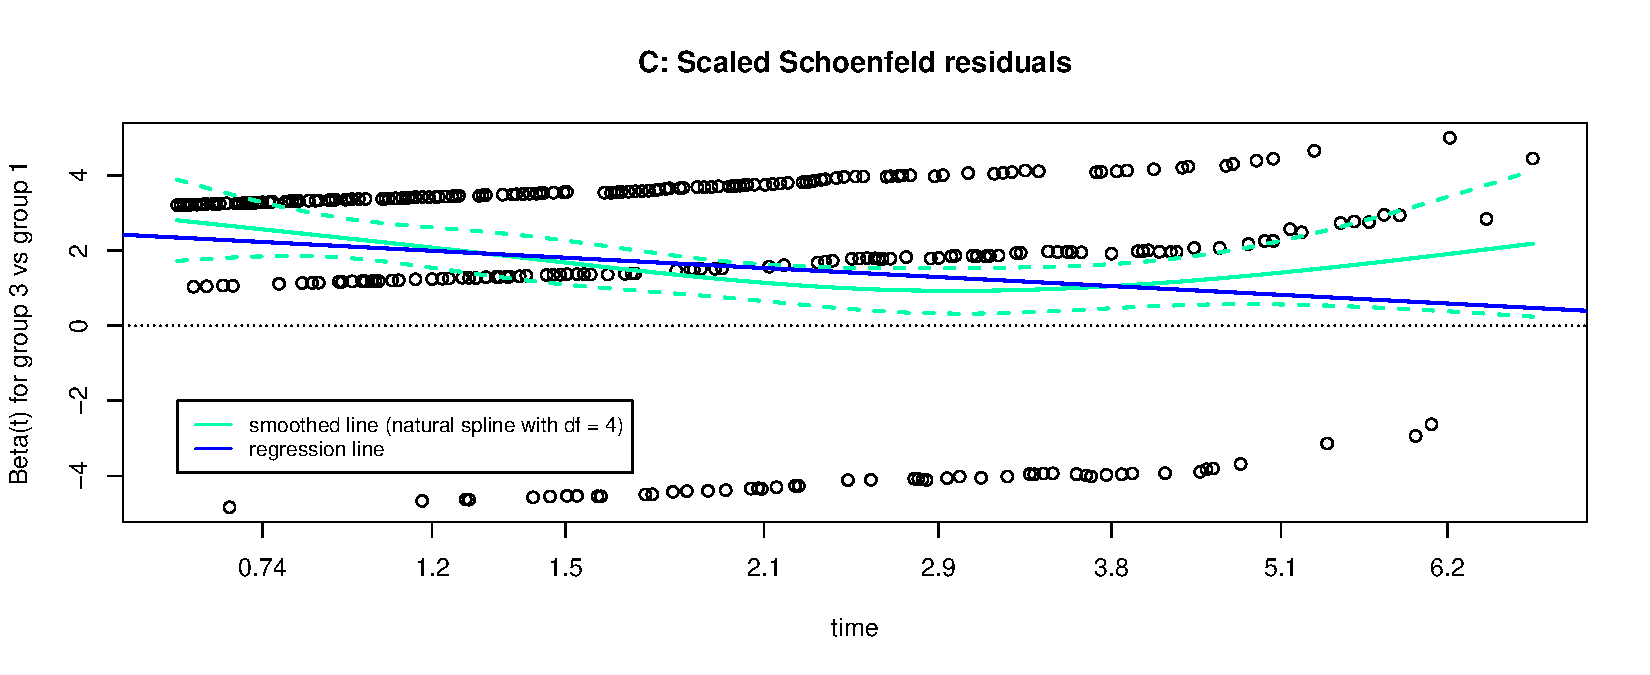
\includegraphics[height=0.29\textheight]{Images/PH_assumption-3} \end{flushleft}

\newpage

\hypertarget{shape-of-the-observed-smoothed-hazard-function}{%
\section{Shape of the observed smoothed hazard
function}\label{shape-of-the-observed-smoothed-hazard-function}}

\hypertarget{should-parametric-survival-models-assuming-a-monotonic-hazard-rate-i.e.-exponential-weibull-gompertz-be-used}{%
\subsection{Should parametric survival models assuming a monotonic
hazard rate (i.e.~exponential, Weibull, Gompertz) be
used?}\label{should-parametric-survival-models-assuming-a-monotonic-hazard-rate-i.e.-exponential-weibull-gompertz-be-used}}

The Figure below represents the smoothed hazard rate over time for each
group. Based on this Figure, an exponential distribution would be
considered suitable if the smoothed hazard rate would be constant over
time (straight vertical line). The Weibull and Gompertz functions would
be considered suitable if the smoothed hazard rate would increase or
decrease monotonically (an upward or downward slope with constant
gradient). More information on which shape of the hazard function can be
estimated by the different parametric survival models can be found
\href{https://devinincerti.com/2019/06/18/parametric_survival.html}{here}.\\
\textbf{Interpretation in this case}: Based on this Figure, one can
discard all three parametric survival models (exponential, Weibull, and
Gompertz), because none of these smoothed hazard rates is constant, or
increases/decreases monotonically over time. Based on this information
and the fact that the PH assumption does likely not hold in this case,
we have decided to fit separate (stratified) parametric survival models
to each group.\\
\textbf{CAUTION}: These smoothed hazard rates apply to the observed
period and do not allow to make inferences about the shape of the hazard
function after the observation period.

\begin{flushleft}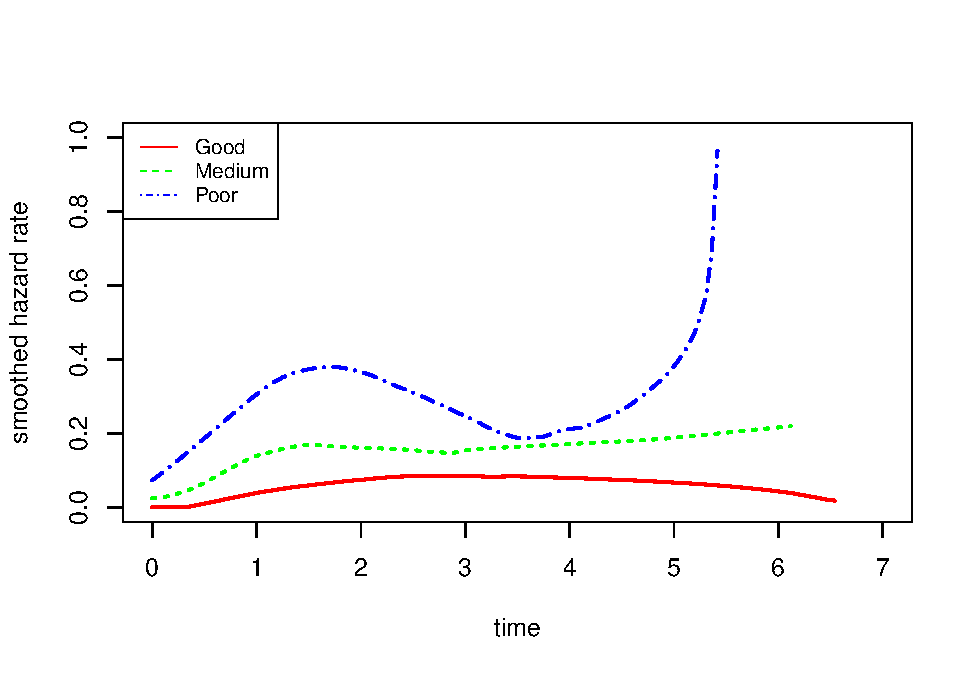
\includegraphics{Images/plot_hr-1} \end{flushleft}

\newpage

\hypertarget{shape-of-the-predicted-hazard-function}{%
\section{Shape of the predicted hazard
function}\label{shape-of-the-predicted-hazard-function}}

The following plots dislay how the hazard rates is estimated through the
different parametric survival models.

\begin{flushleft}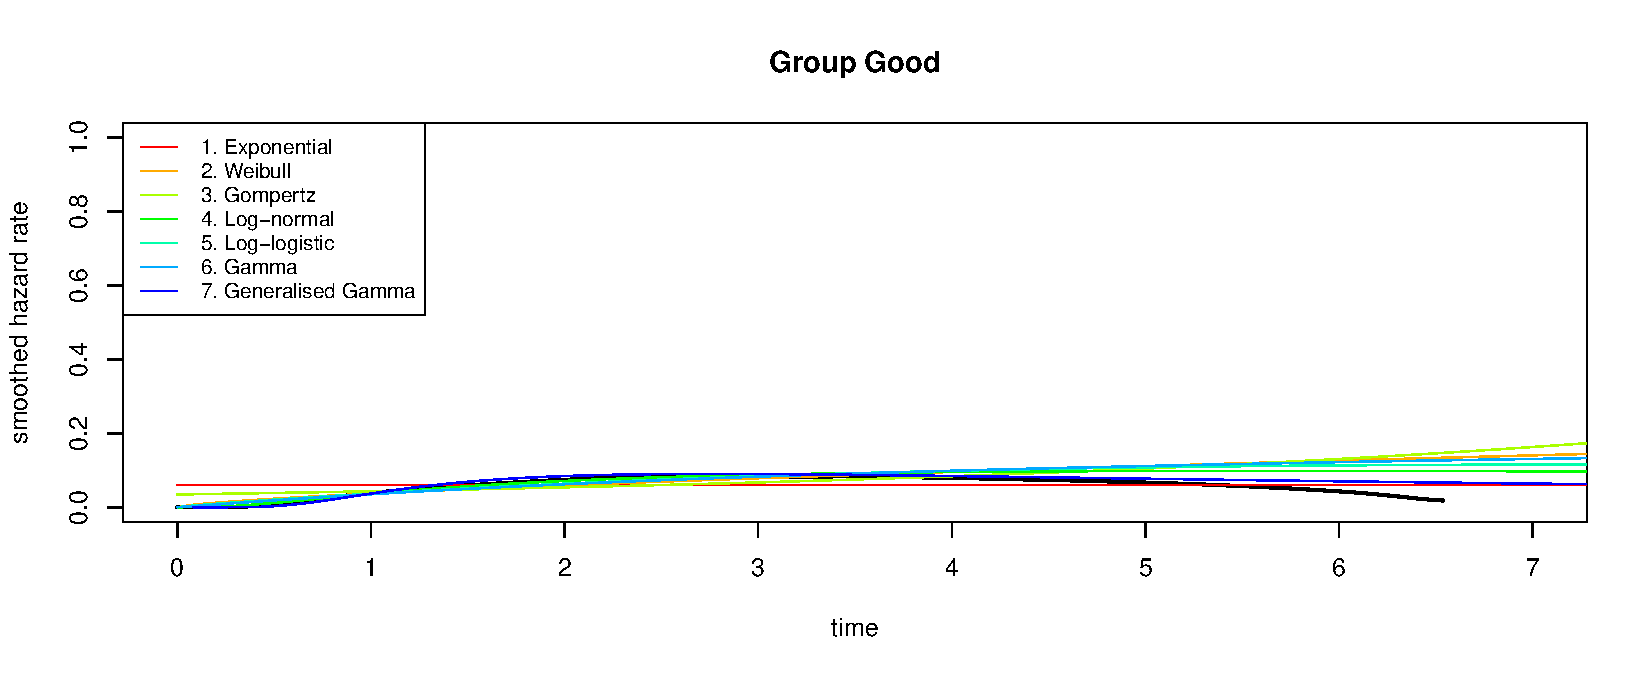
\includegraphics[height=0.29\textheight]{Images/plot_haz_pred-1} \end{flushleft}

\begin{flushleft}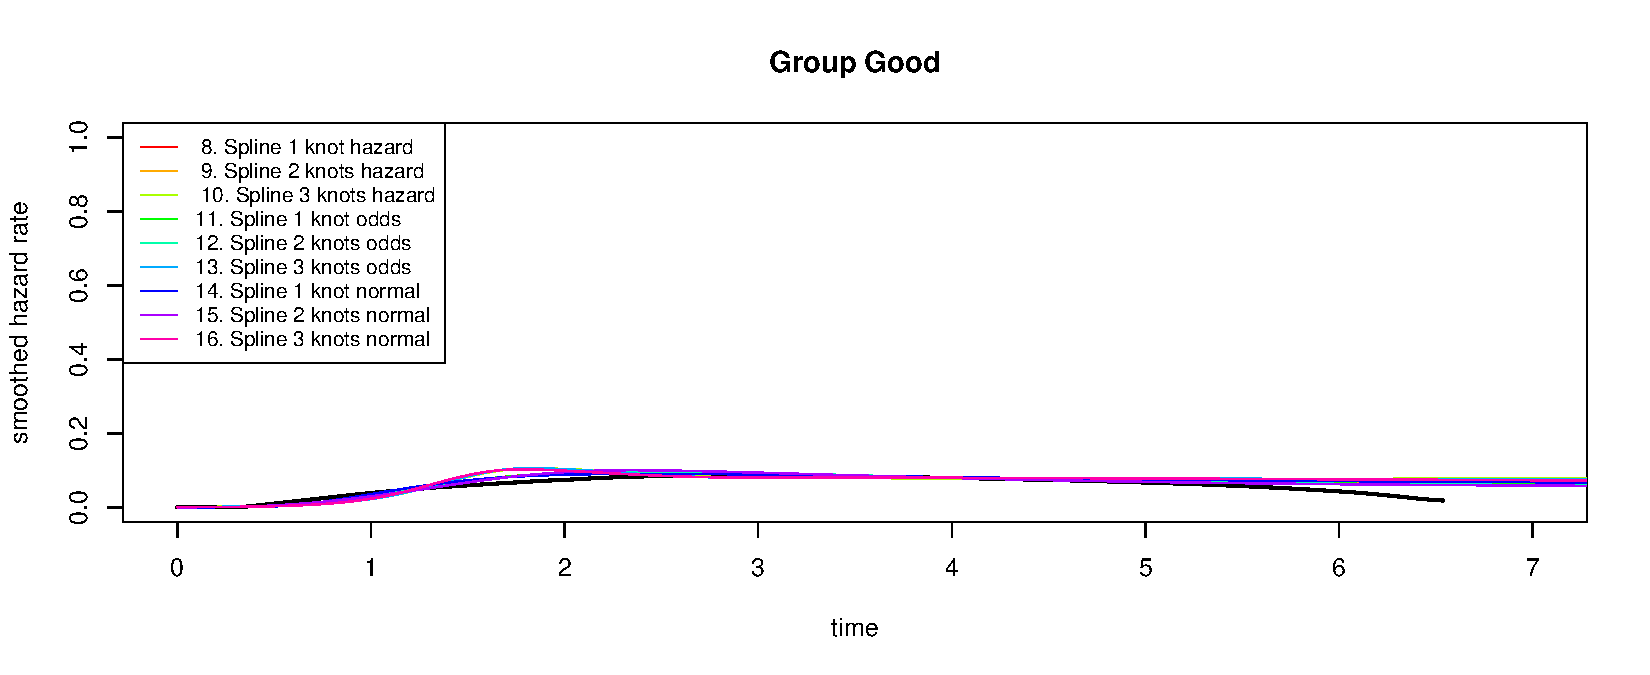
\includegraphics[height=0.29\textheight]{Images/plot_haz_pred-2} \end{flushleft}

\begin{flushleft}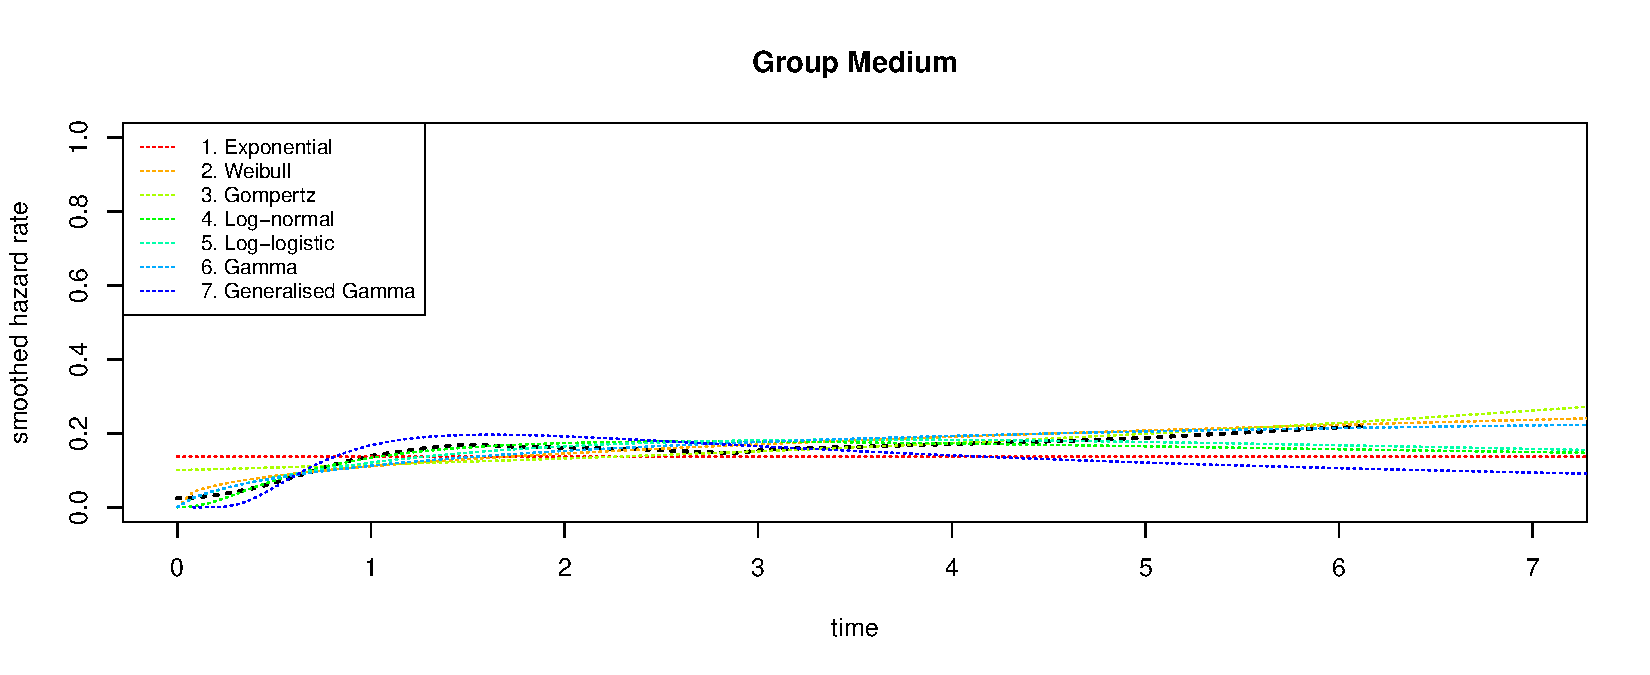
\includegraphics[height=0.29\textheight]{Images/plot_haz_pred-3} \end{flushleft}

\begin{flushleft}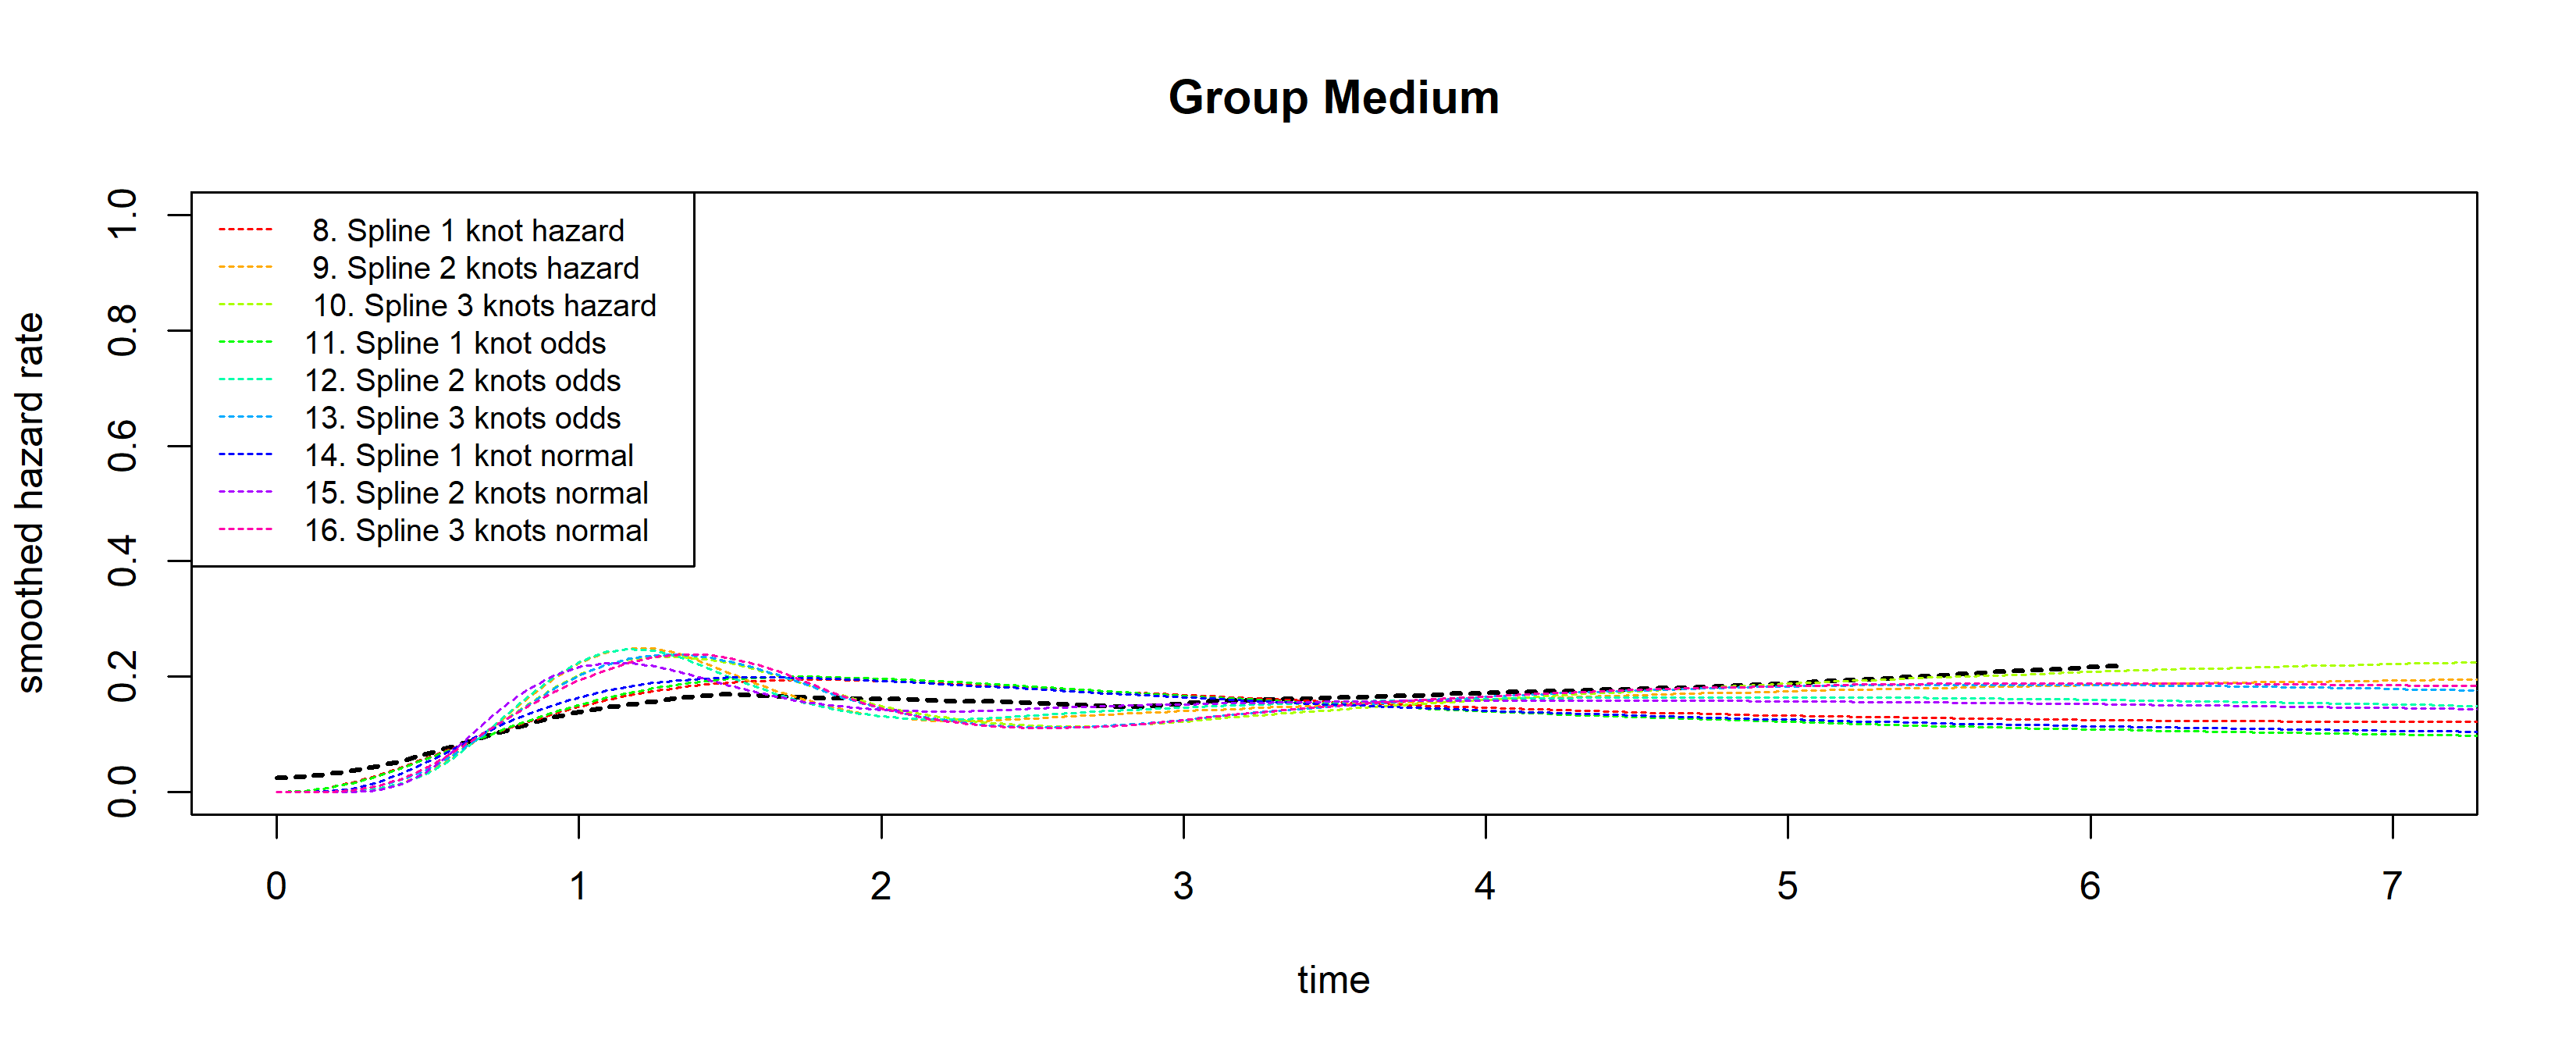
\includegraphics[height=0.29\textheight]{Images/plot_haz_pred-4} \end{flushleft}

\begin{flushleft}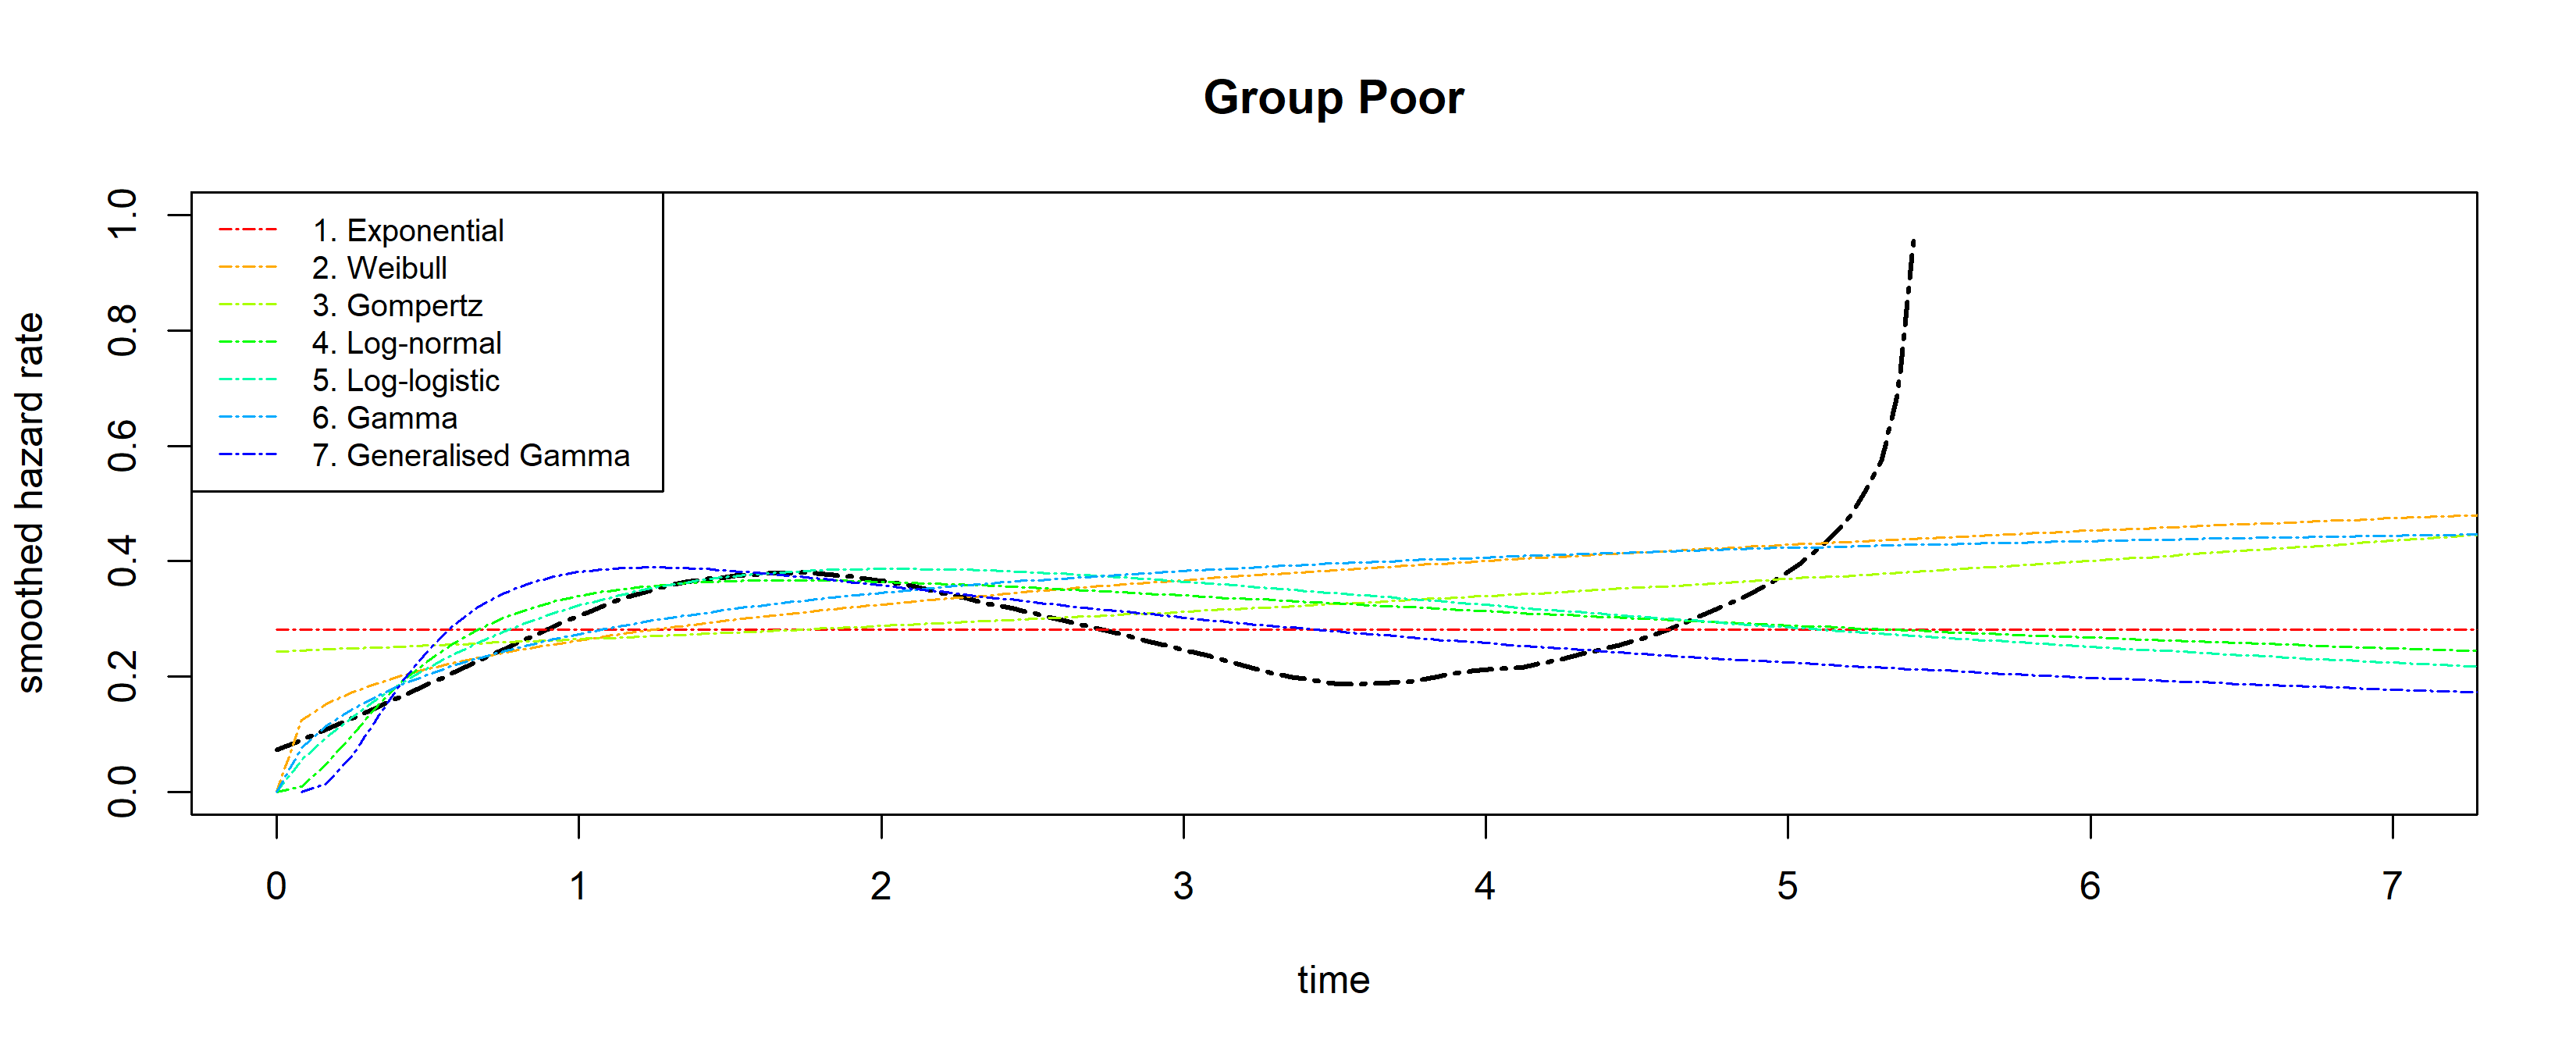
\includegraphics[height=0.29\textheight]{Images/plot_haz_pred-5} \end{flushleft}

\begin{flushleft}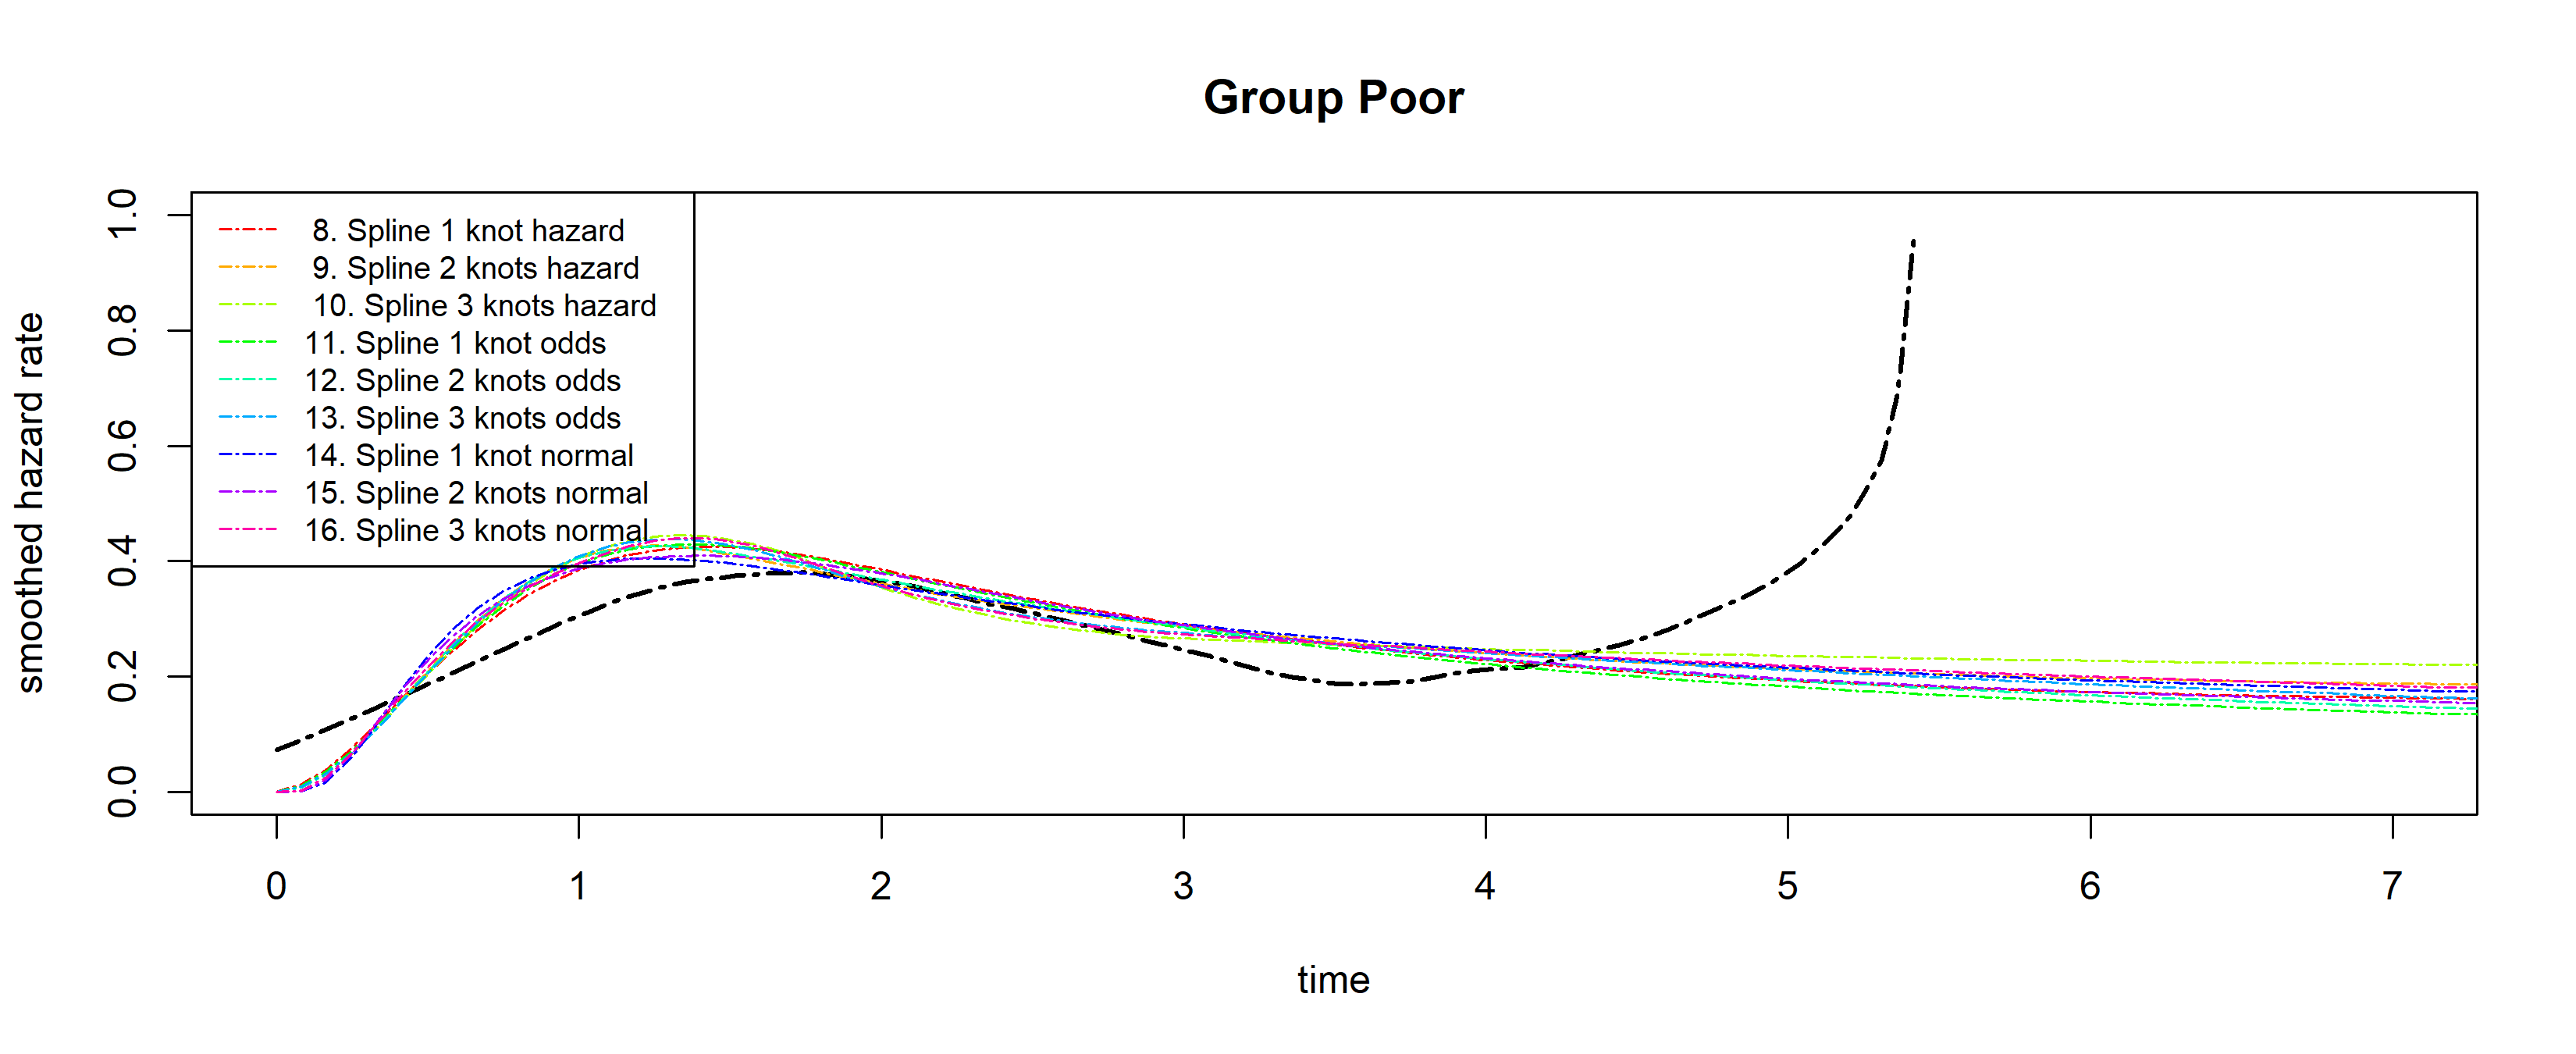
\includegraphics[height=0.29\textheight]{Images/plot_haz_pred-6} \end{flushleft}

\newpage

\hypertarget{standard-parametric-models}{%
\section{Standard parametric models?}\label{standard-parametric-models}}

\hypertarget{do-standard-parametric-models-provide-an-appropriate-fit-to-the-data}{%
\subsection{Do standard parametric models provide an appropriate fit to
the
data?}\label{do-standard-parametric-models-provide-an-appropriate-fit-to-the-data}}

The circle displays the colours that are attributed to each parametric
survival model in the graphs on the following pages.\\
The Table below displays the goodness-of-fit statistics for each
parametric survival model, ordered from `best' fitting to less well
fitting, based on the Akaike Information Criterion (AIC). The AIC and
Bayesian Information Criterion (BIC) provide a measure of the relative
fit of each model to the data, while penalising for the number of
parameter included in the fitted models. The lower the AIC or BIC, the
better the relative fit of a model compared to other fitted models.\\
\textbf{Interpretation in this case}: Based on this Table, one can
conclude that the generalised gamma and log-normal parametric survival
models fit the data best relative to the other fitted models, according
to the AIC.\\
\textbf{CAUTION}: These goodness-of-fit statistics only apply to the
observed period of time and do not allow to issue statements about the
suitability of the extrapolated survival by these fitted models beyond
the observation period.

In the following pages, three plots per fitted parametric survival model
are displayed to support the visual inspection of the fit of the models
to the observed data. Figure A shows the Kaplan-Meier curves (black and
gray) versus the fitted parametric survival models (colour). Figure B
displays a comparison of the smoothed hazard rates based on the
empirical data (black and gray) versus the estimated transition
probabilities (colour, based on the fitted parametric survival models).
In all Figures A and B, the Kaplan-Meier curves and the smoothed hazard
rates are the same. Figure C shows a specific diagnostic plot for each
fitted parametric survival model. For all these plots, the rule is: the
closer the coloured lines are to the black and grey lines, the better.\\
\textbf{Interpretation in this case}: Based on these plots, one can see
that the generalised gamma and log-normal parametric survival models
seem to estimate the transition probabilities the most closely, but
there are still some discrepancies between observed and estimated
transition probabilities, especially in the `Poor' and `Medium' group.
This can be explained by the changing direction of the hazard rates in
the `Poor' group over time. It increases until approximately year 2,
then decreases until approximately year 5, and then increases again.
Standard parametric survival models are not able to capture multiple
changes in the hazard function over time, hence, more flexible models
which allow for multiple changes in the hazard functions may be
required.\\
\textbf{CAUTION}: These observations only apply to the observed period
of time and do not allow to issue statements about the suitability of
the extrapolated survival by these fitted models beyond the observation
period. Additionally, the shape of the hazard function (smoothed
transition rates) at the end of the observed period may be affected by
the low number of observations in the tail of the Kaplan-Meier curves.
One should therefore consider these changing hazard at the end of the
observed period cautiously.

\begin{flushleft}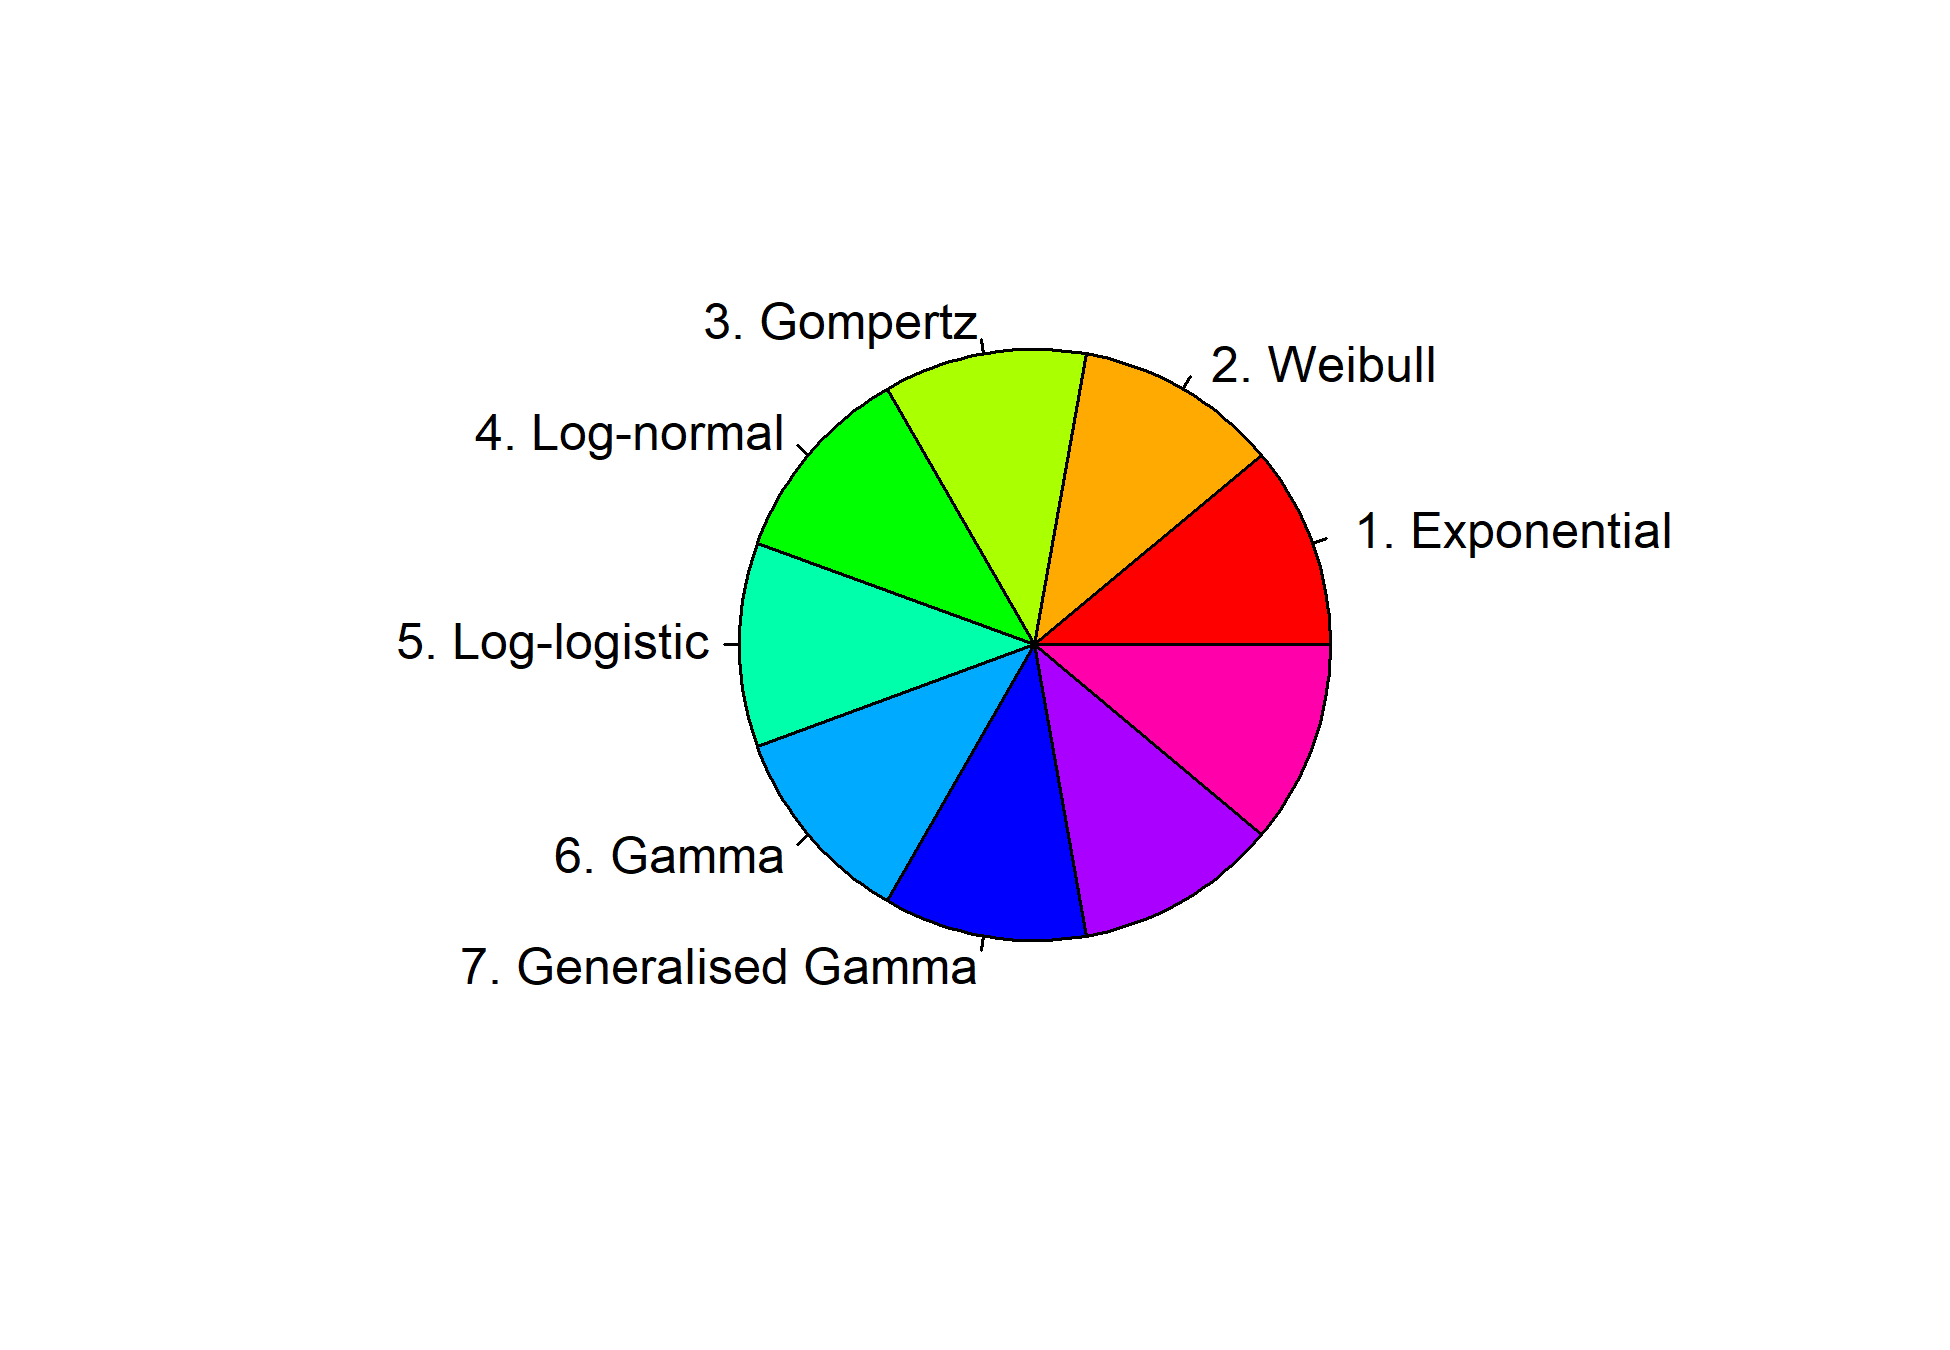
\includegraphics{Images/plot_parametric-1} \end{flushleft}

\begin{table}[H]
\centering
\begin{tabular}{lrr}
\toprule
Model & AIC & BIC\\
\midrule
\cellcolor{gray!6}{7. Generalised Gamma} & \cellcolor{gray!6}{1589.049} & \cellcolor{gray!6}{1629.826}\\
4. Log-normal & 1592.880 & 1620.066\\
\cellcolor{gray!6}{5. Log-logistic} & \cellcolor{gray!6}{1609.294} & \cellcolor{gray!6}{1636.479}\\
6. Gamma & 1621.982 & 1649.167\\
\cellcolor{gray!6}{2. Weibull} & \cellcolor{gray!6}{1632.618} & \cellcolor{gray!6}{1659.803}\\
3. Gompertz & 1660.954 & 1688.140\\
\cellcolor{gray!6}{1. Exponential} & \cellcolor{gray!6}{1668.212} & \cellcolor{gray!6}{1681.805}\\
\bottomrule
\end{tabular}
\end{table}

\hypertarget{exponential}{%
\subsection{Exponential}\label{exponential}}

\begin{flushleft}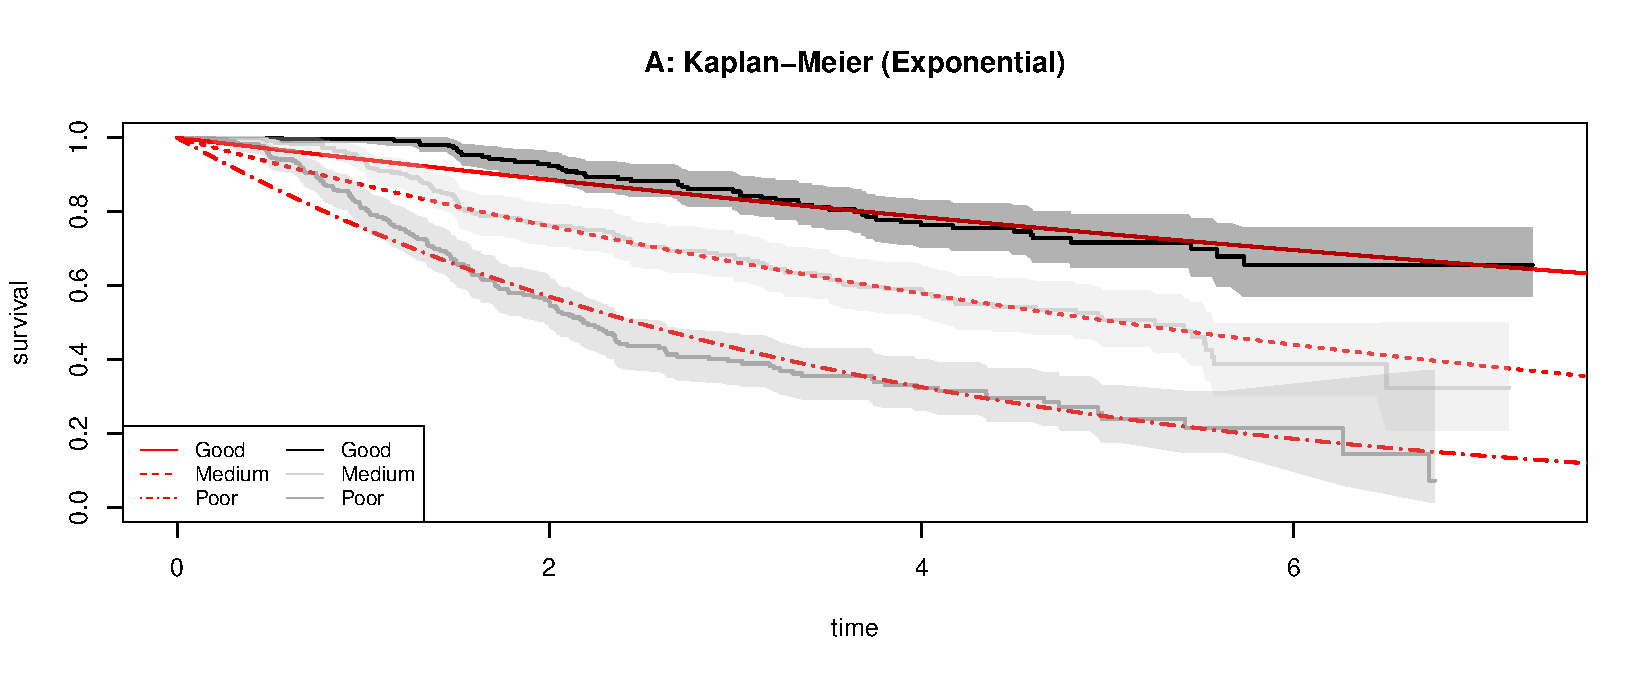
\includegraphics[height=0.3\textheight]{Images/expo-1} \end{flushleft}

\begin{flushleft}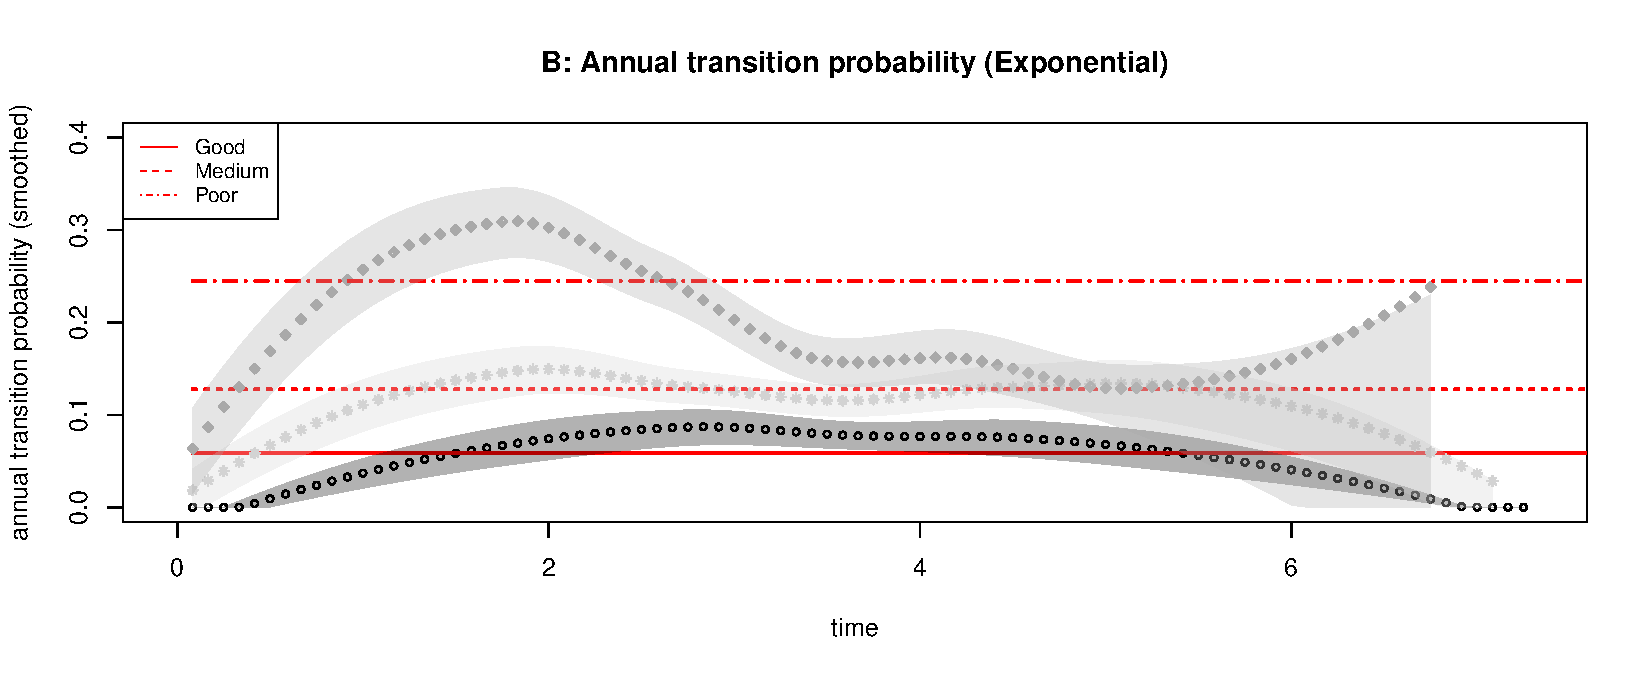
\includegraphics[height=0.3\textheight]{Images/expo-2} \end{flushleft}

\begin{flushleft}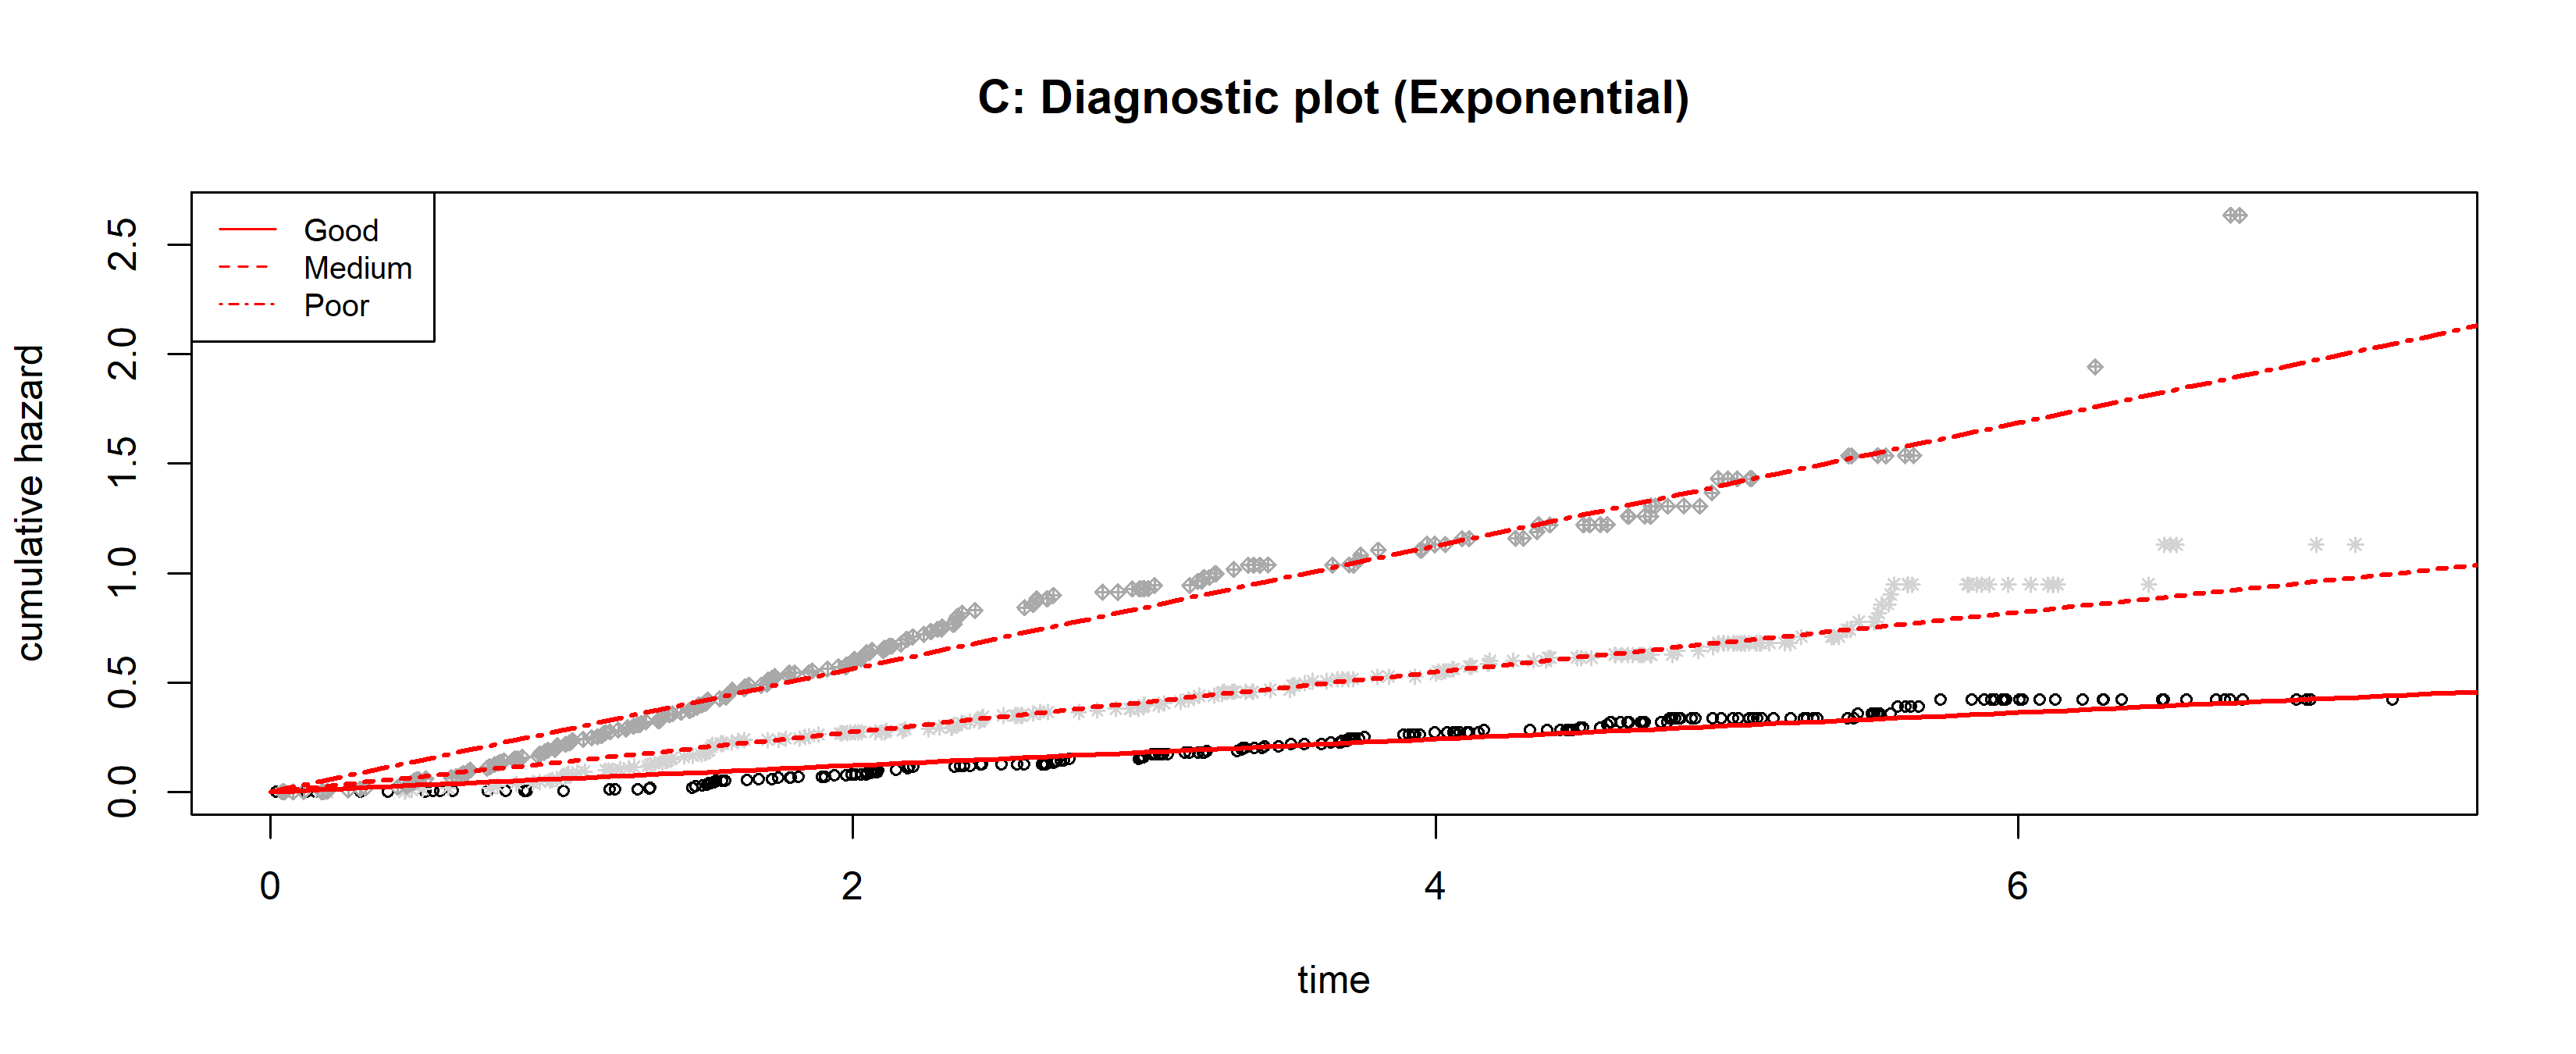
\includegraphics[height=0.3\textheight]{Images/expo-3} \end{flushleft}

\hypertarget{weibull}{%
\subsection{Weibull}\label{weibull}}

\begin{flushleft}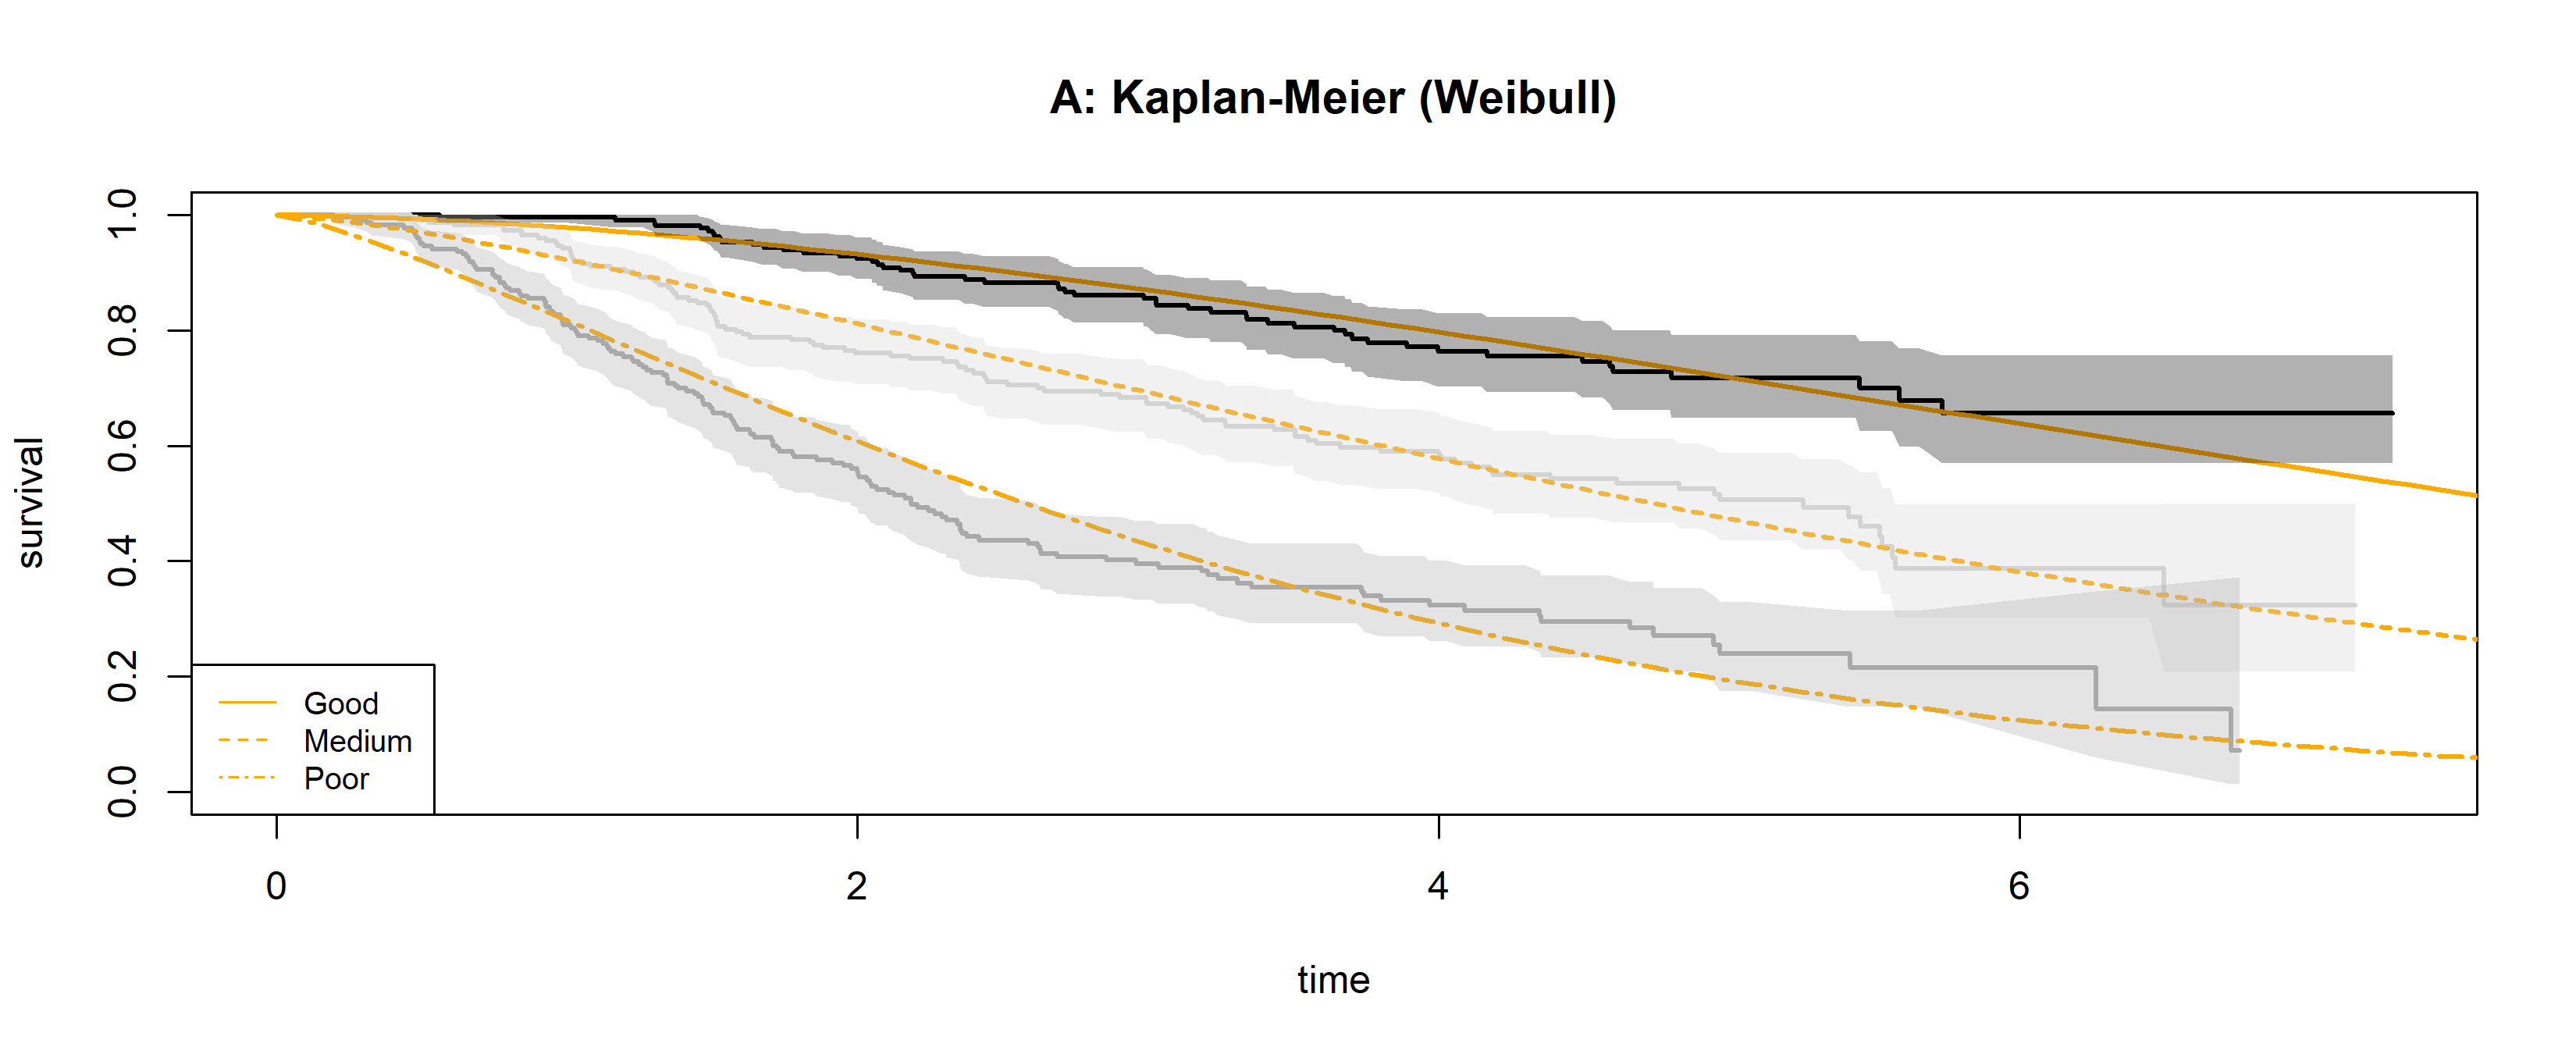
\includegraphics[height=0.3\textheight]{Images/weib-1} \end{flushleft}

\begin{flushleft}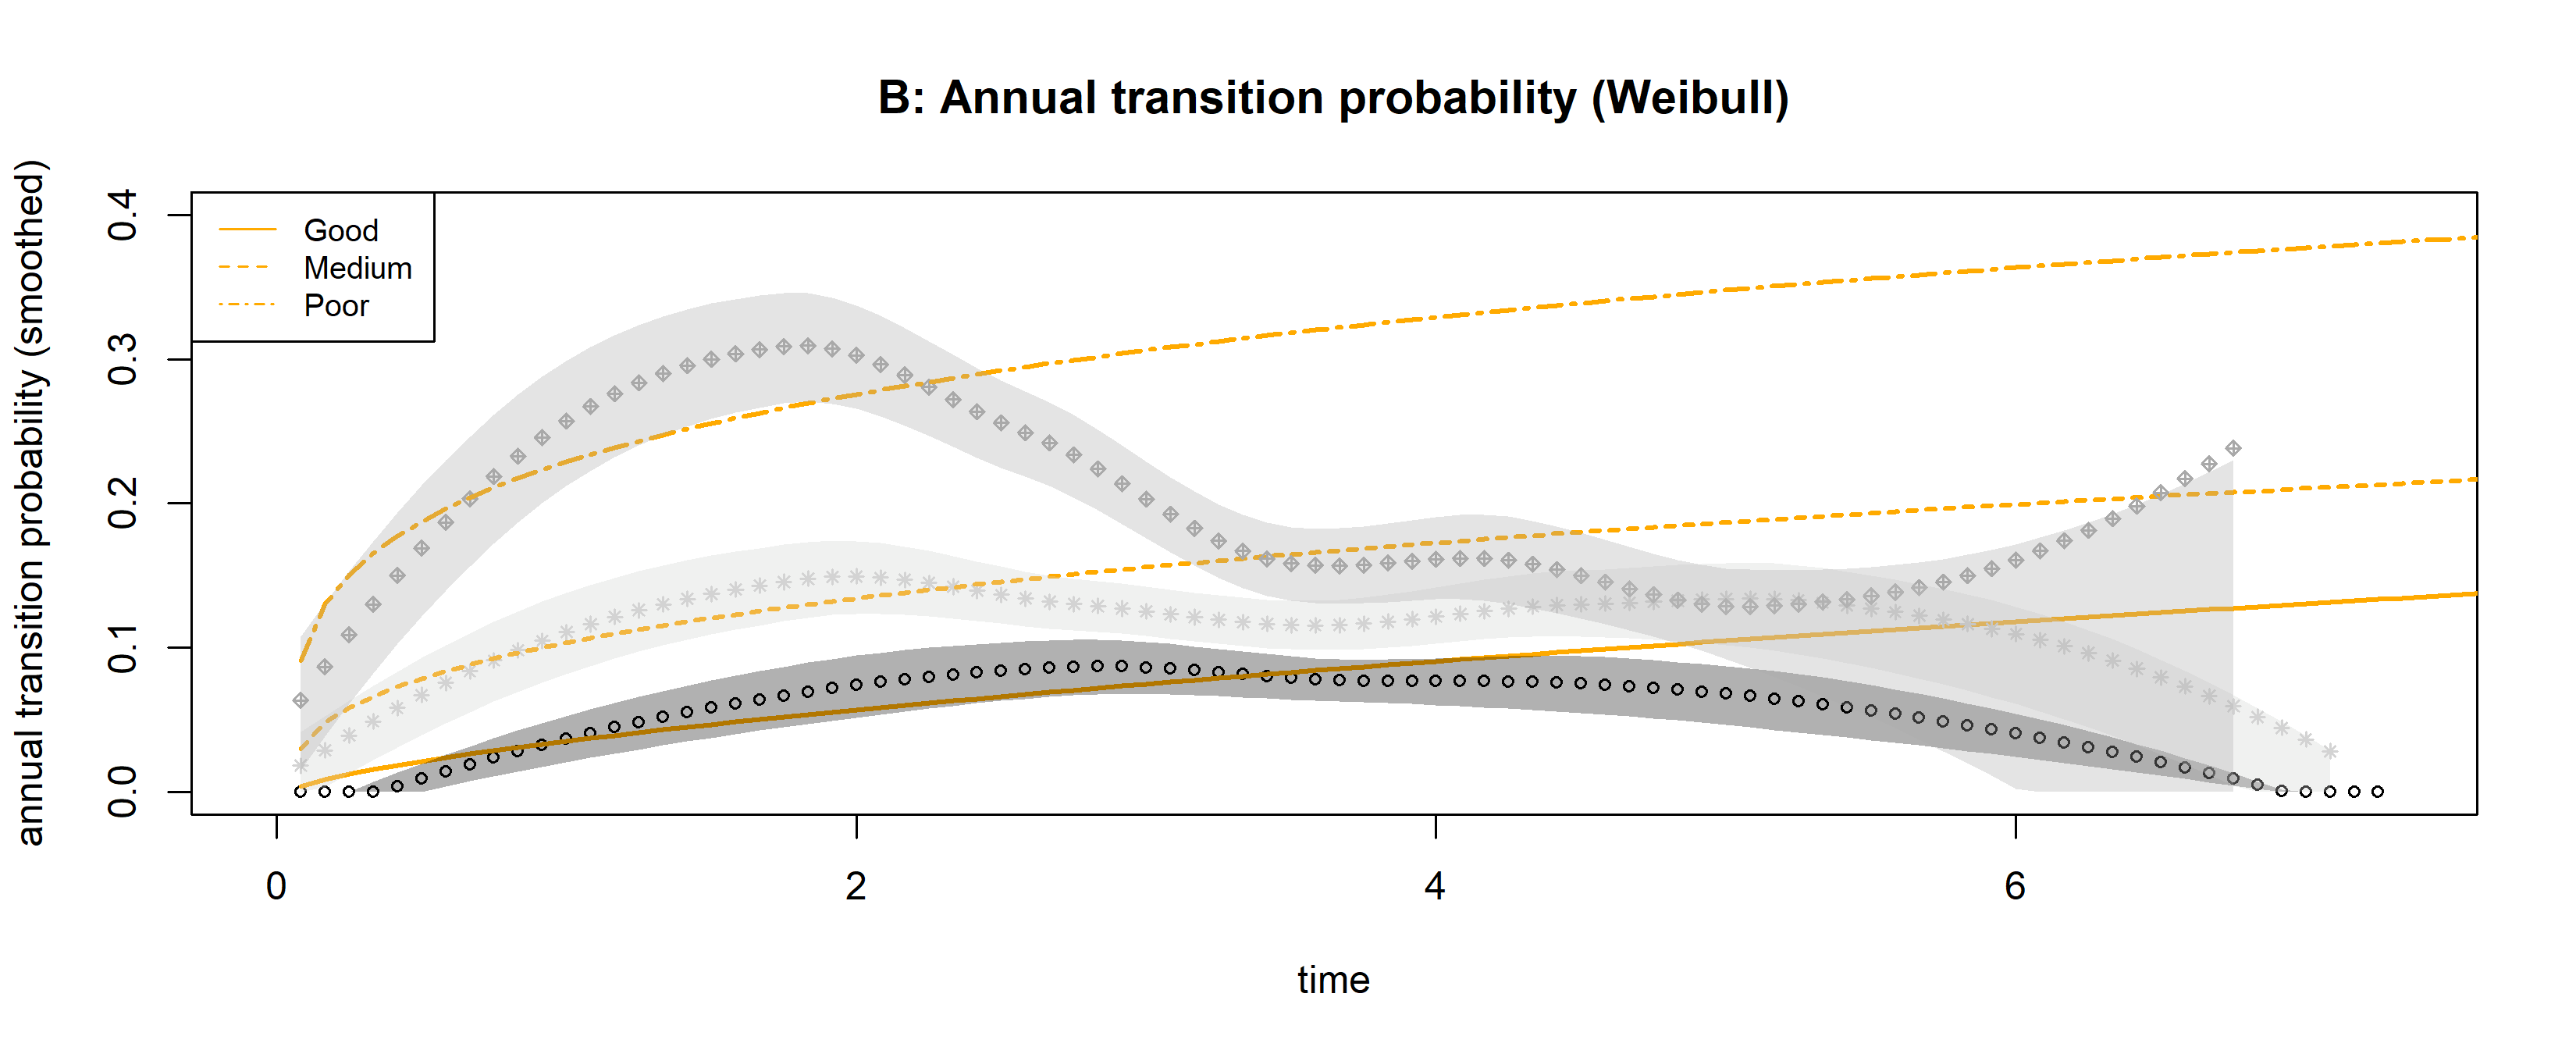
\includegraphics[height=0.3\textheight]{Images/weib-2} \end{flushleft}

\begin{flushleft}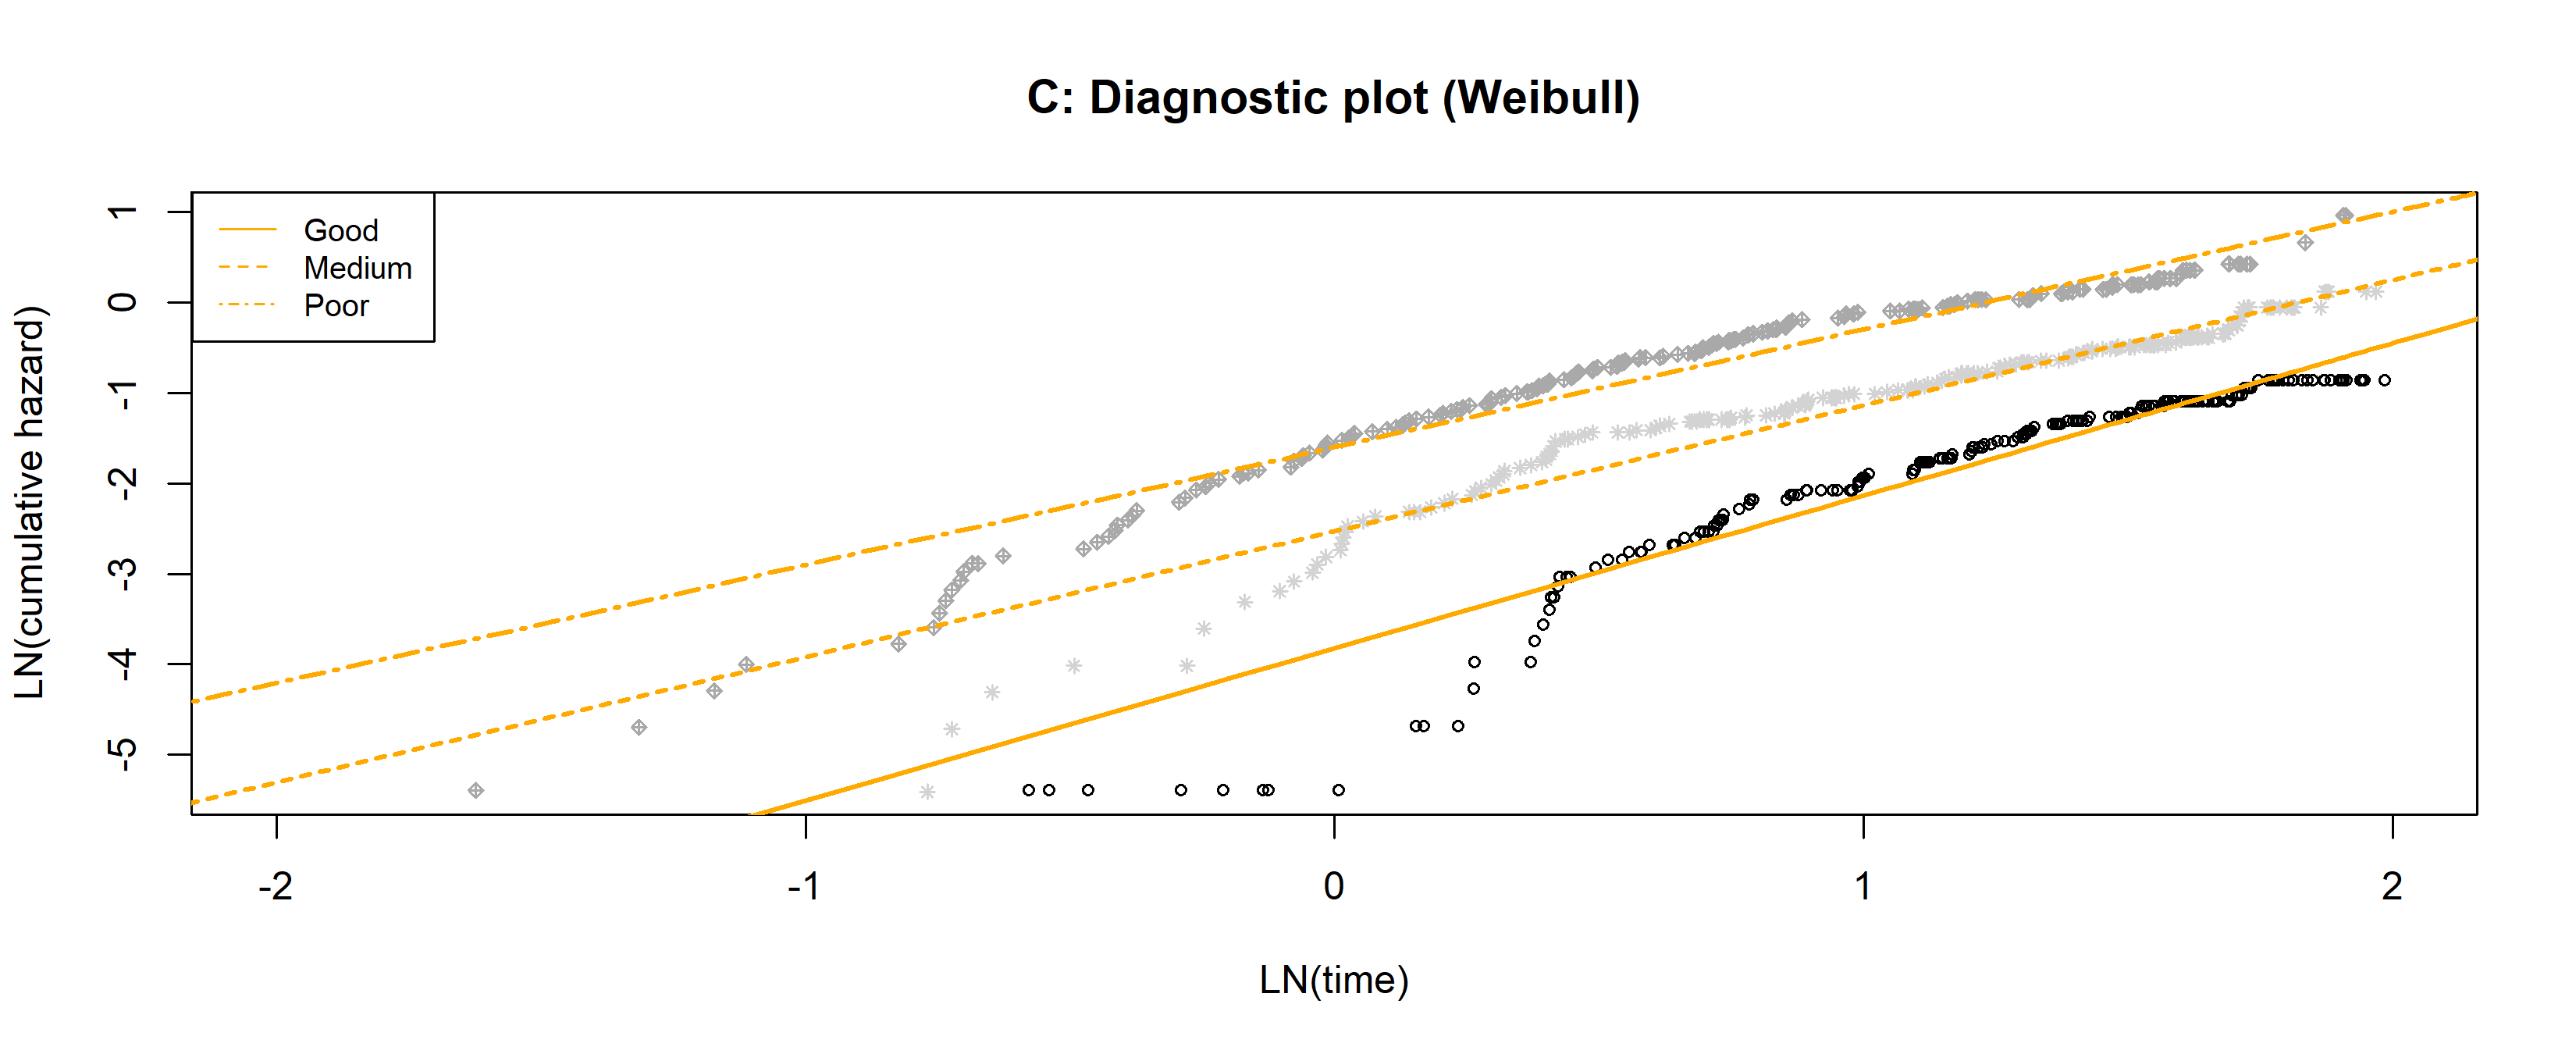
\includegraphics[height=0.3\textheight]{Images/weib-3} \end{flushleft}

\hypertarget{gompertz}{%
\subsection{Gompertz}\label{gompertz}}

\begin{flushleft}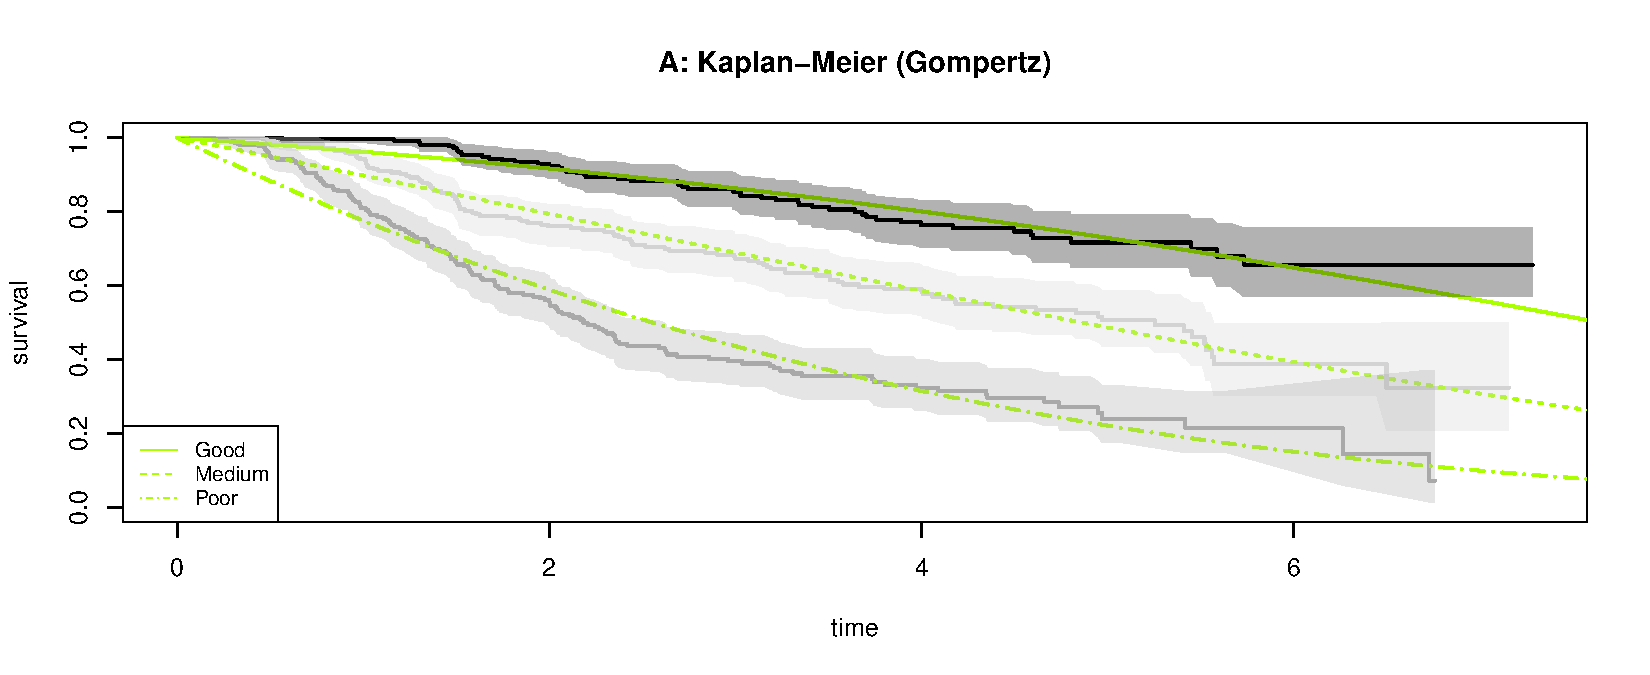
\includegraphics[height=0.3\textheight]{Images/gom-1} \end{flushleft}

\begin{flushleft}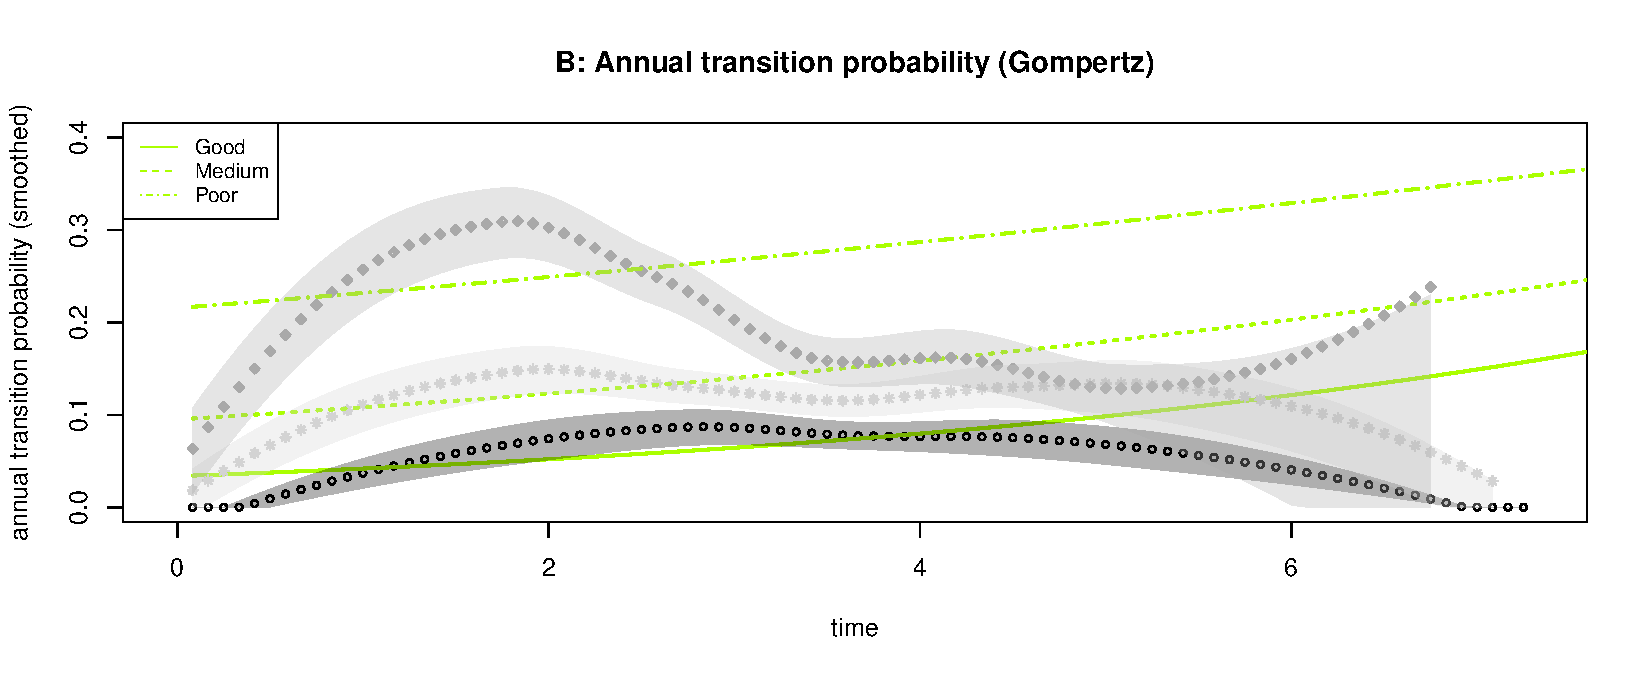
\includegraphics[height=0.3\textheight]{Images/gom-2} \end{flushleft}

\begin{flushleft}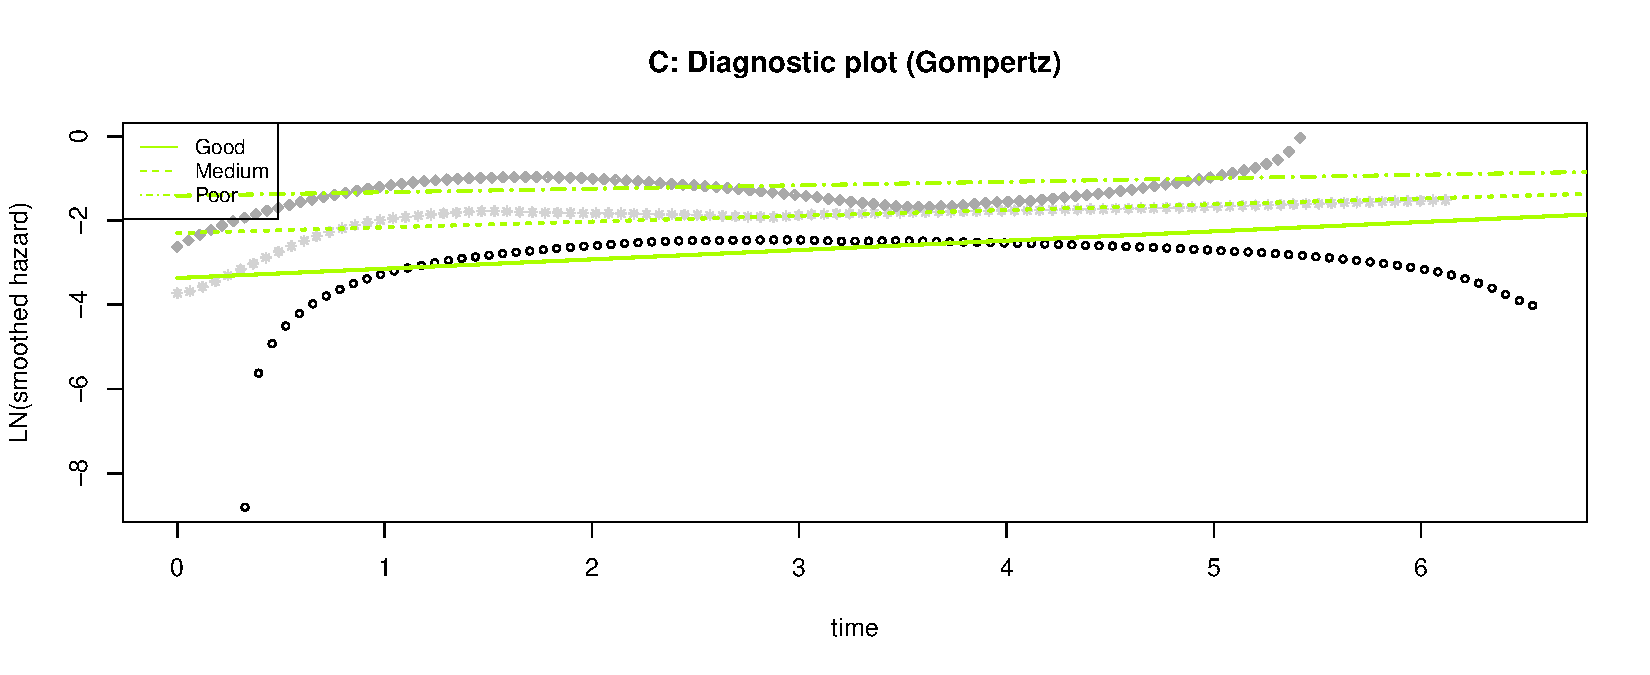
\includegraphics[height=0.3\textheight]{Images/gom-3} \end{flushleft}

\hypertarget{log-normal}{%
\subsection{Log-normal}\label{log-normal}}

\begin{flushleft}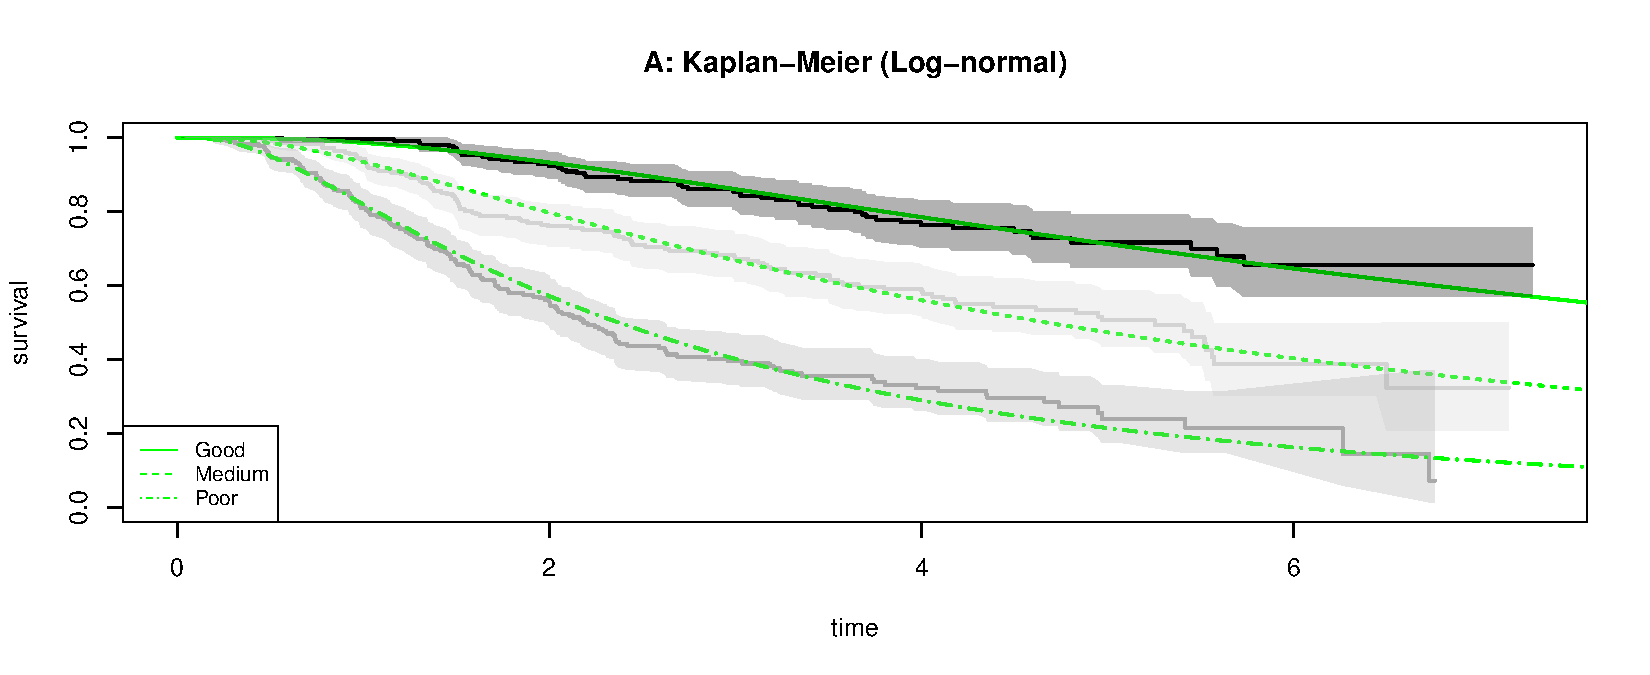
\includegraphics[height=0.3\textheight]{Images/lnorm-1} \end{flushleft}

\begin{flushleft}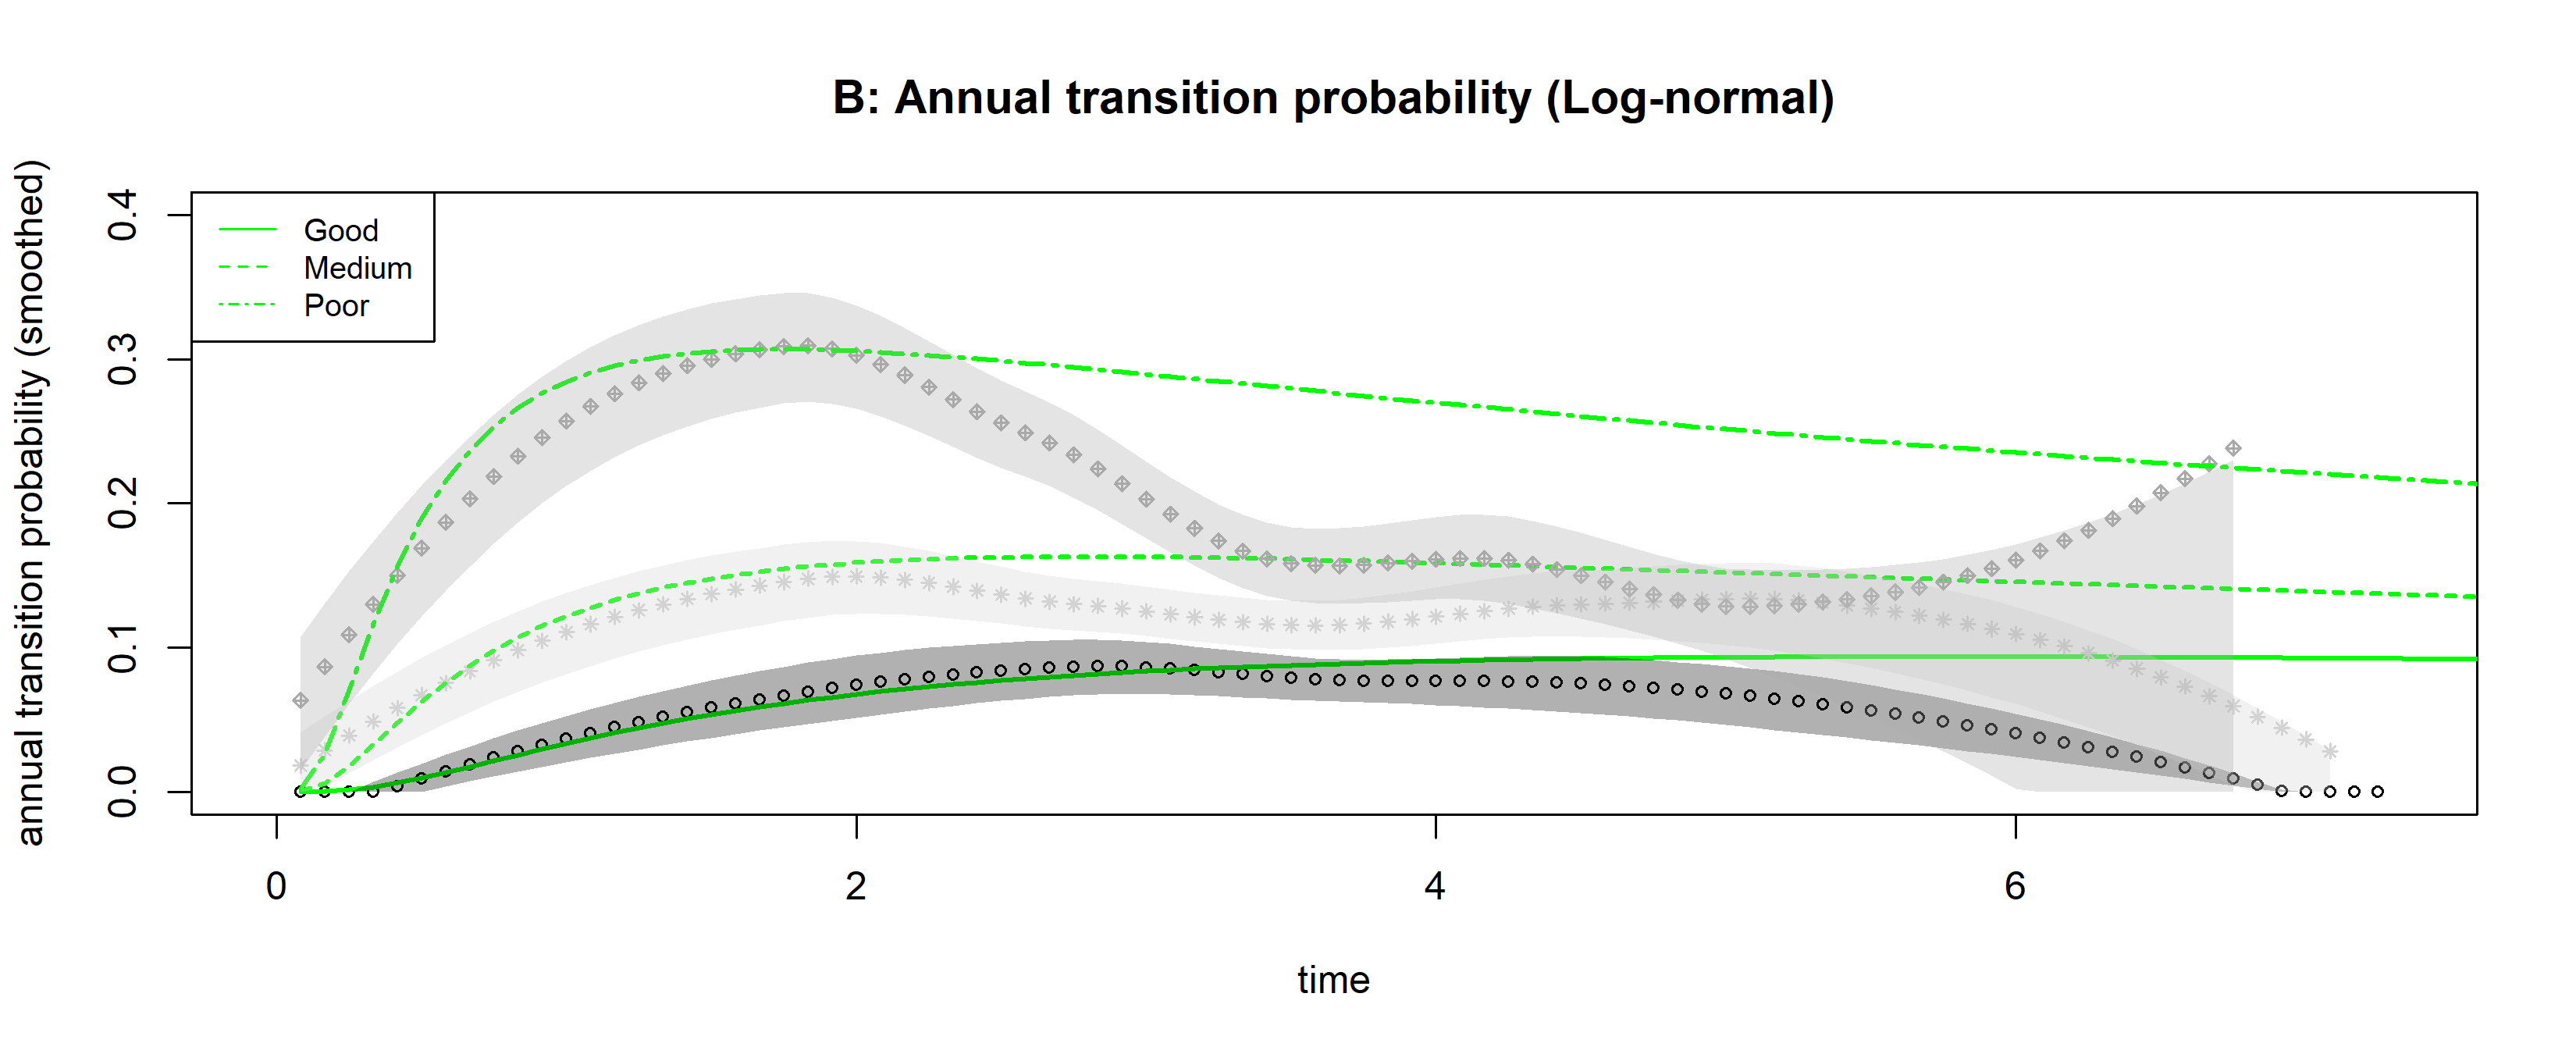
\includegraphics[height=0.3\textheight]{Images/lnorm-2} \end{flushleft}

\begin{flushleft}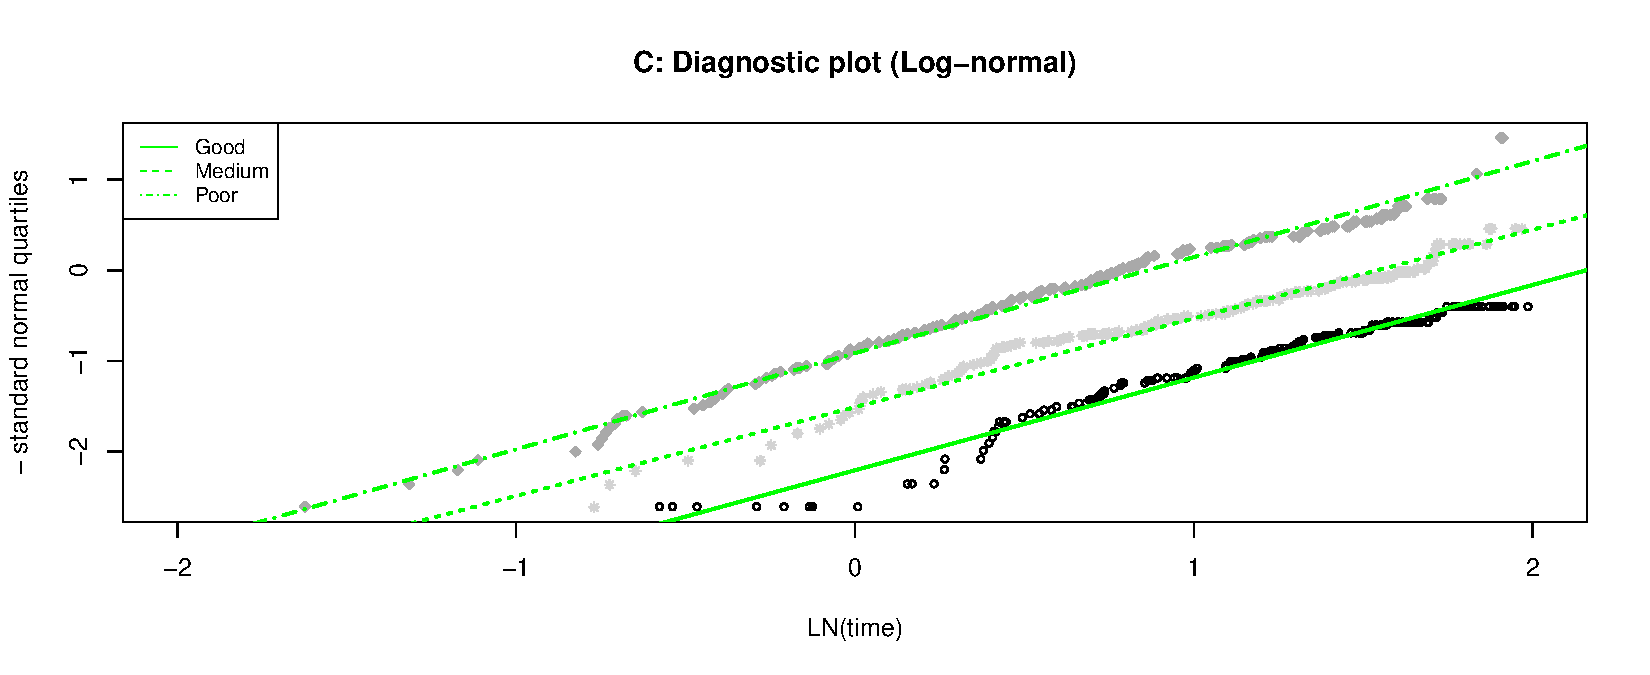
\includegraphics[height=0.3\textheight]{Images/lnorm-3} \end{flushleft}

\hypertarget{log-logistic}{%
\subsection{Log-logistic}\label{log-logistic}}

\begin{flushleft}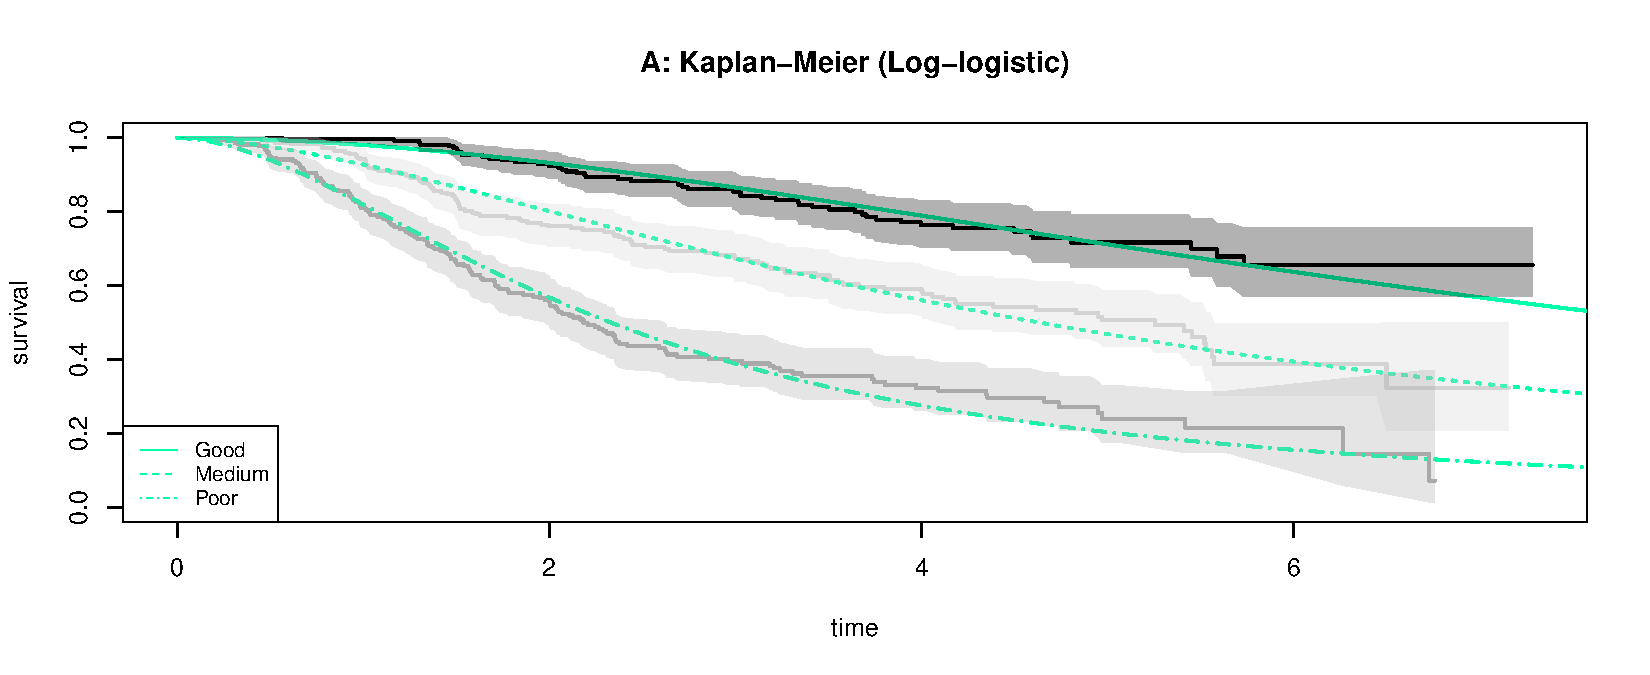
\includegraphics[height=0.3\textheight]{Images/llog-1} \end{flushleft}

\begin{flushleft}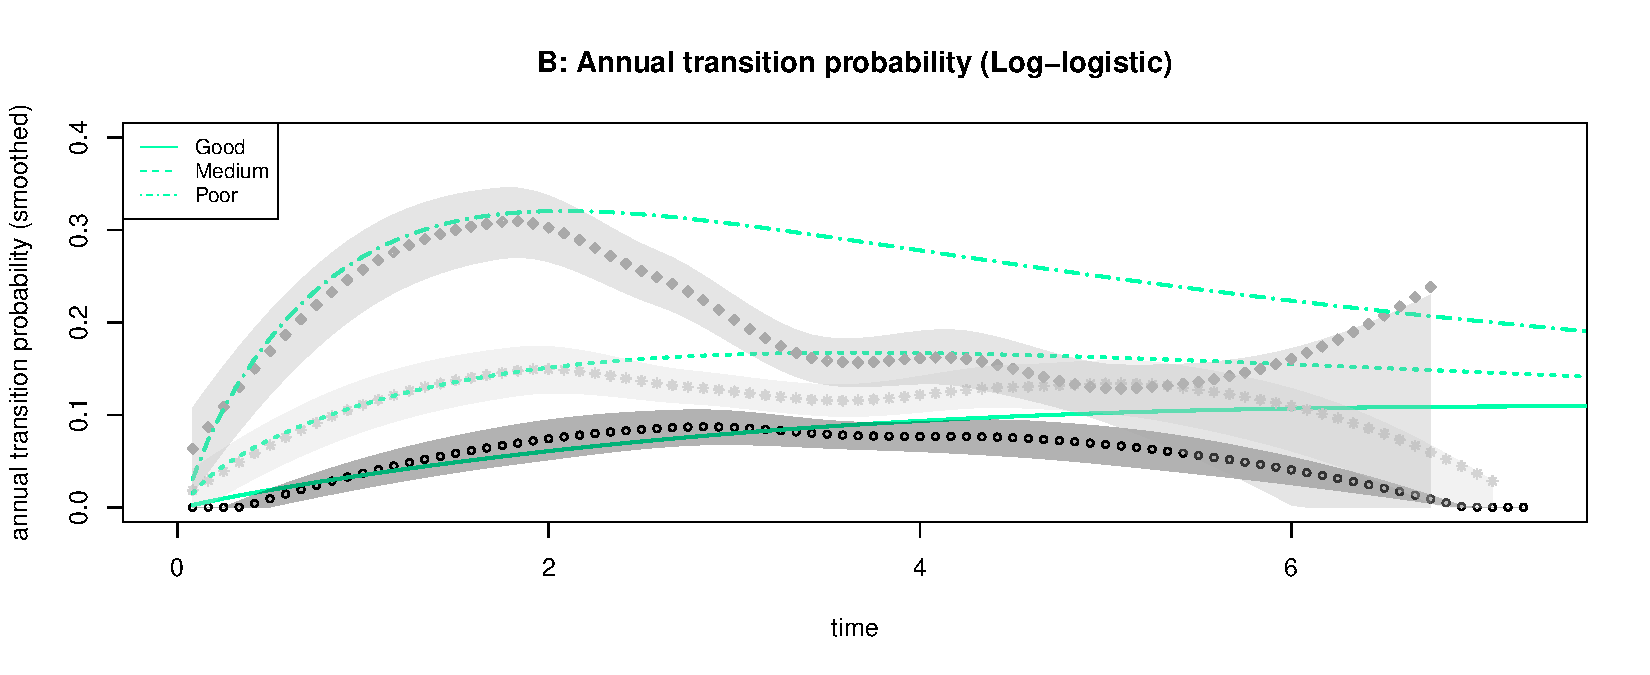
\includegraphics[height=0.3\textheight]{Images/llog-2} \end{flushleft}

\begin{flushleft}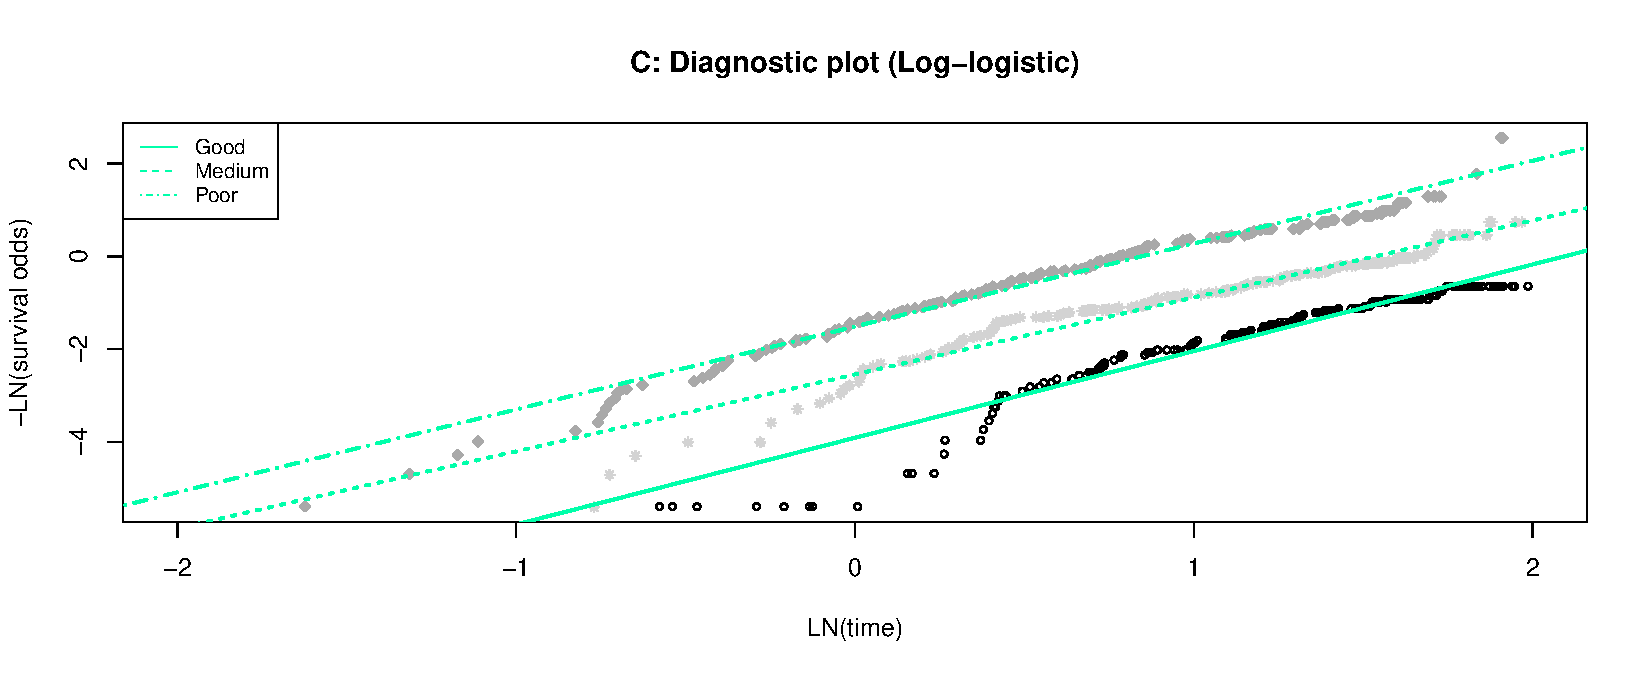
\includegraphics[height=0.3\textheight]{Images/llog-3} \end{flushleft}

\hypertarget{gamma}{%
\subsection{Gamma}\label{gamma}}

\begin{flushleft}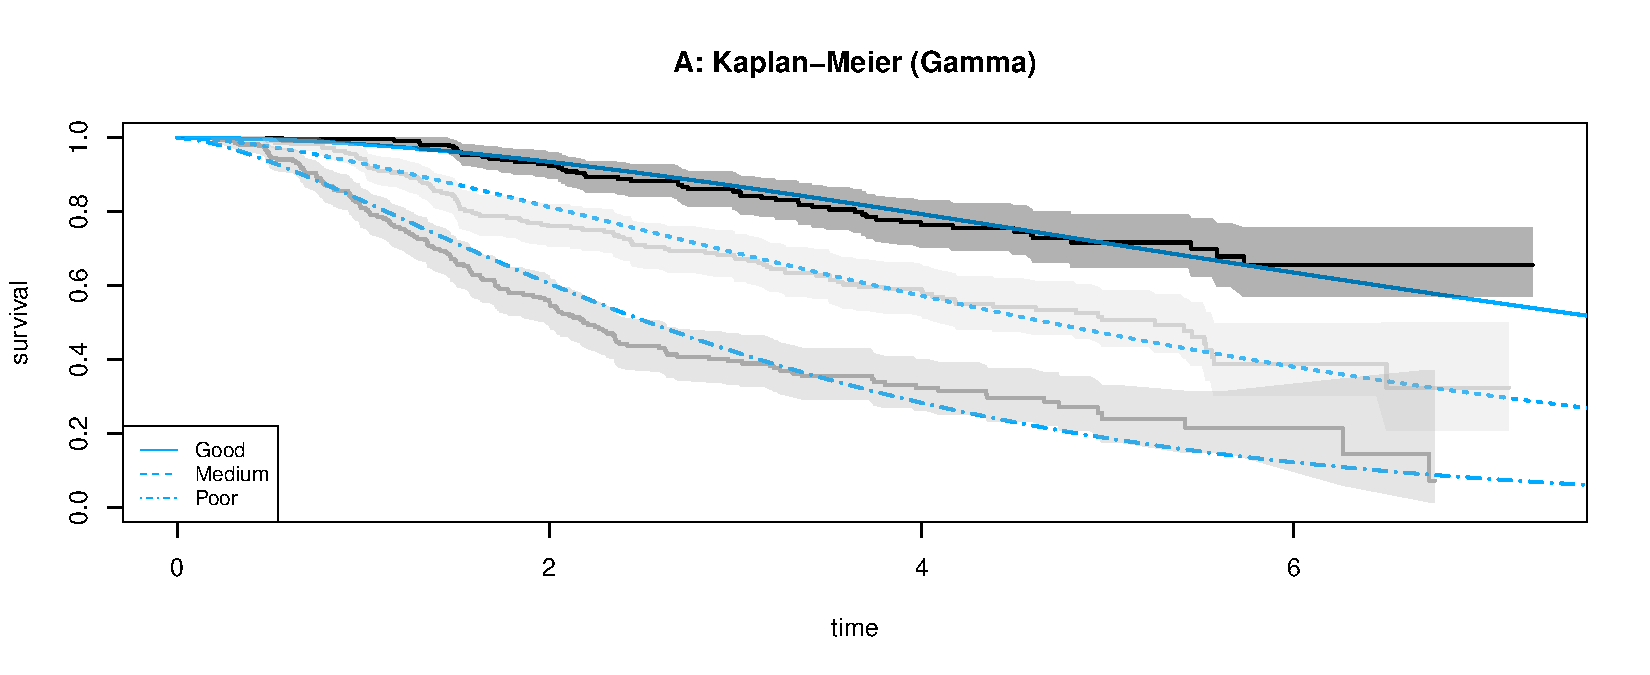
\includegraphics[height=0.3\textheight]{Images/gam-1} \end{flushleft}

\begin{flushleft}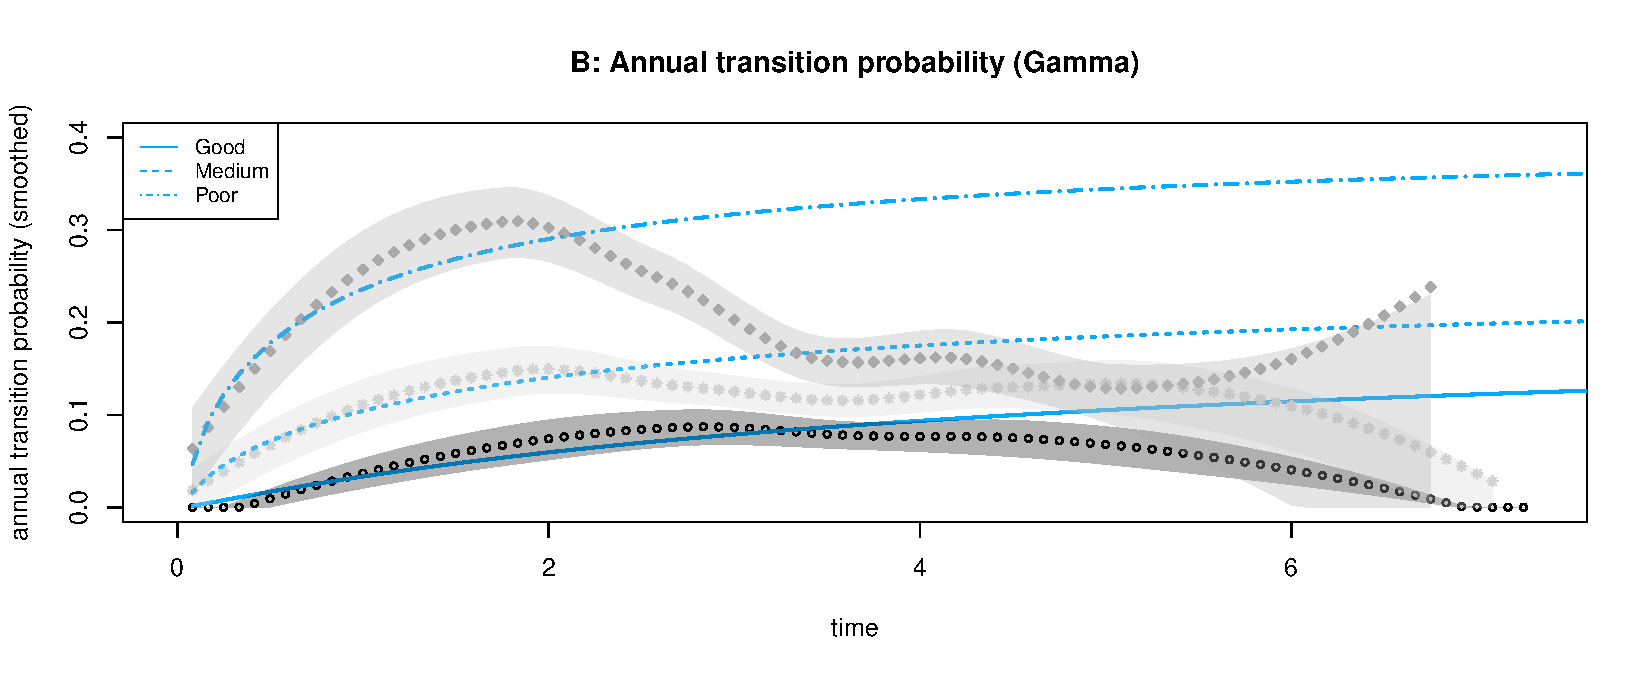
\includegraphics[height=0.3\textheight]{Images/gam-2} \end{flushleft}

\begin{flushleft}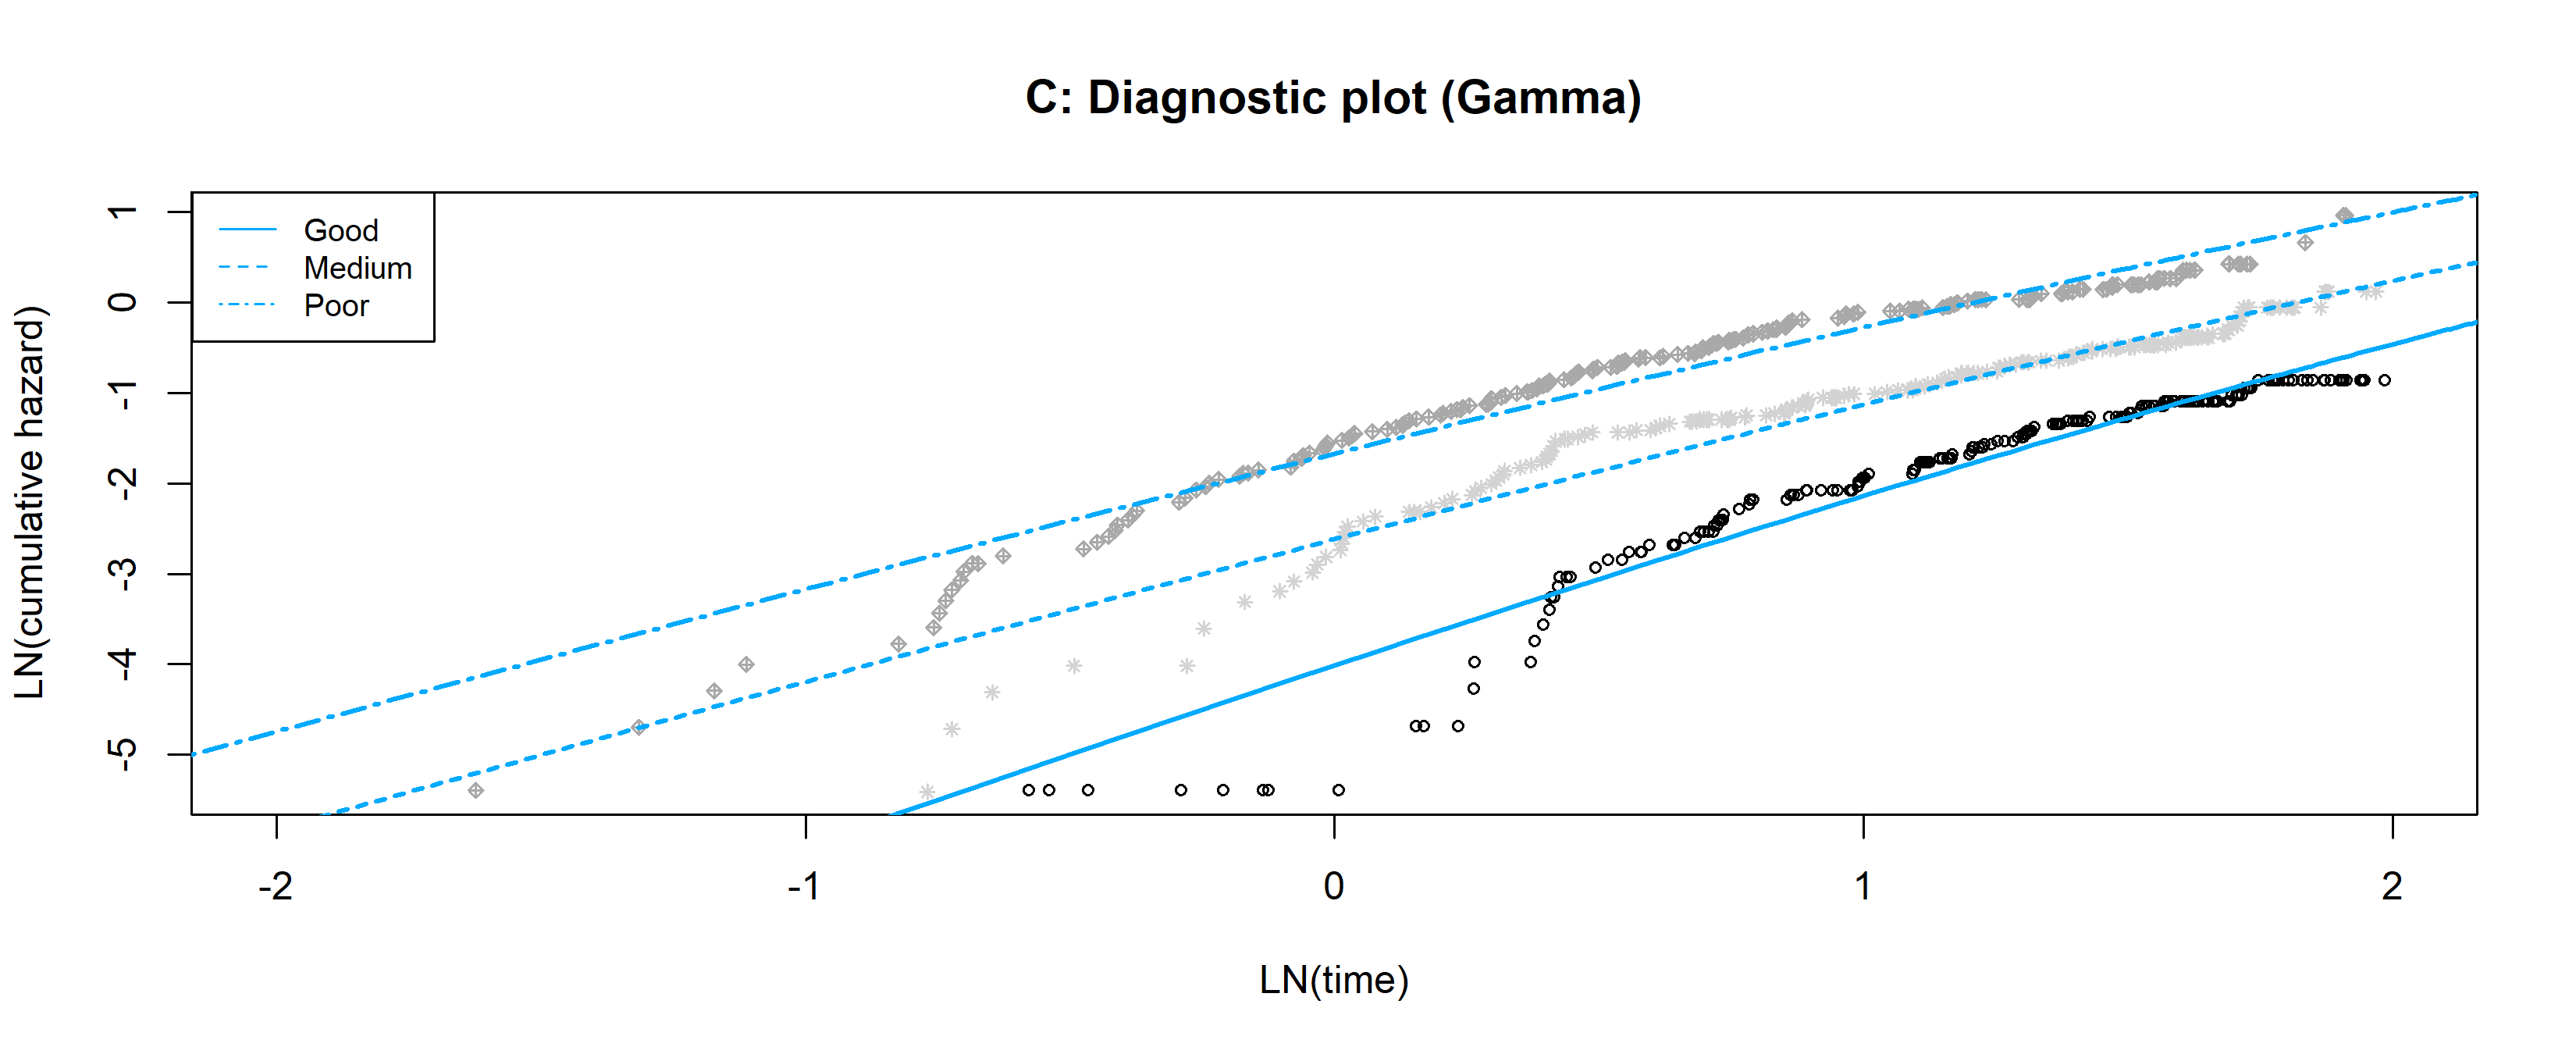
\includegraphics[height=0.3\textheight]{Images/gam-3} \end{flushleft}

\hypertarget{generalised-gamma}{%
\subsection{Generalised Gamma}\label{generalised-gamma}}

\begin{flushleft}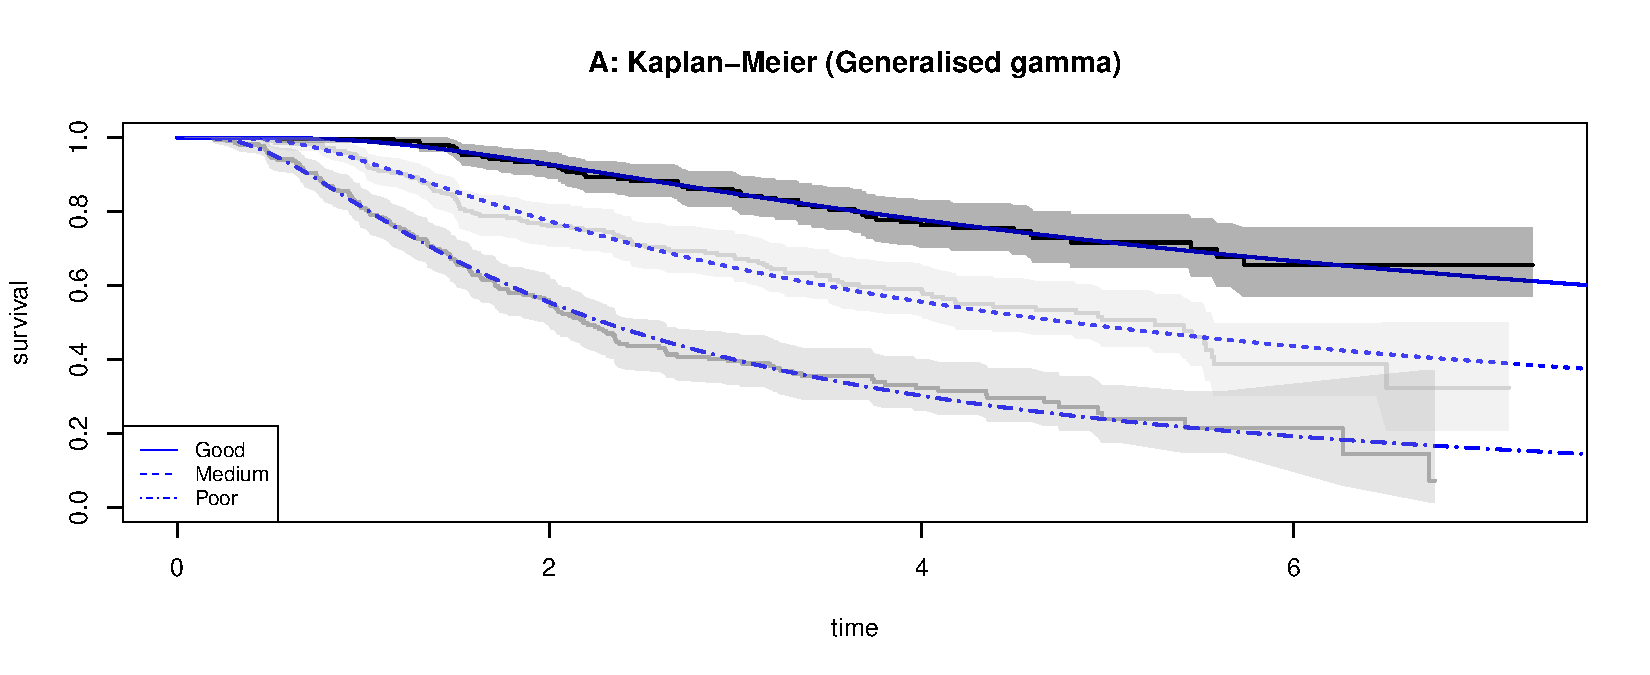
\includegraphics[height=0.3\textheight]{Images/ggam-1} \end{flushleft}

\begin{flushleft}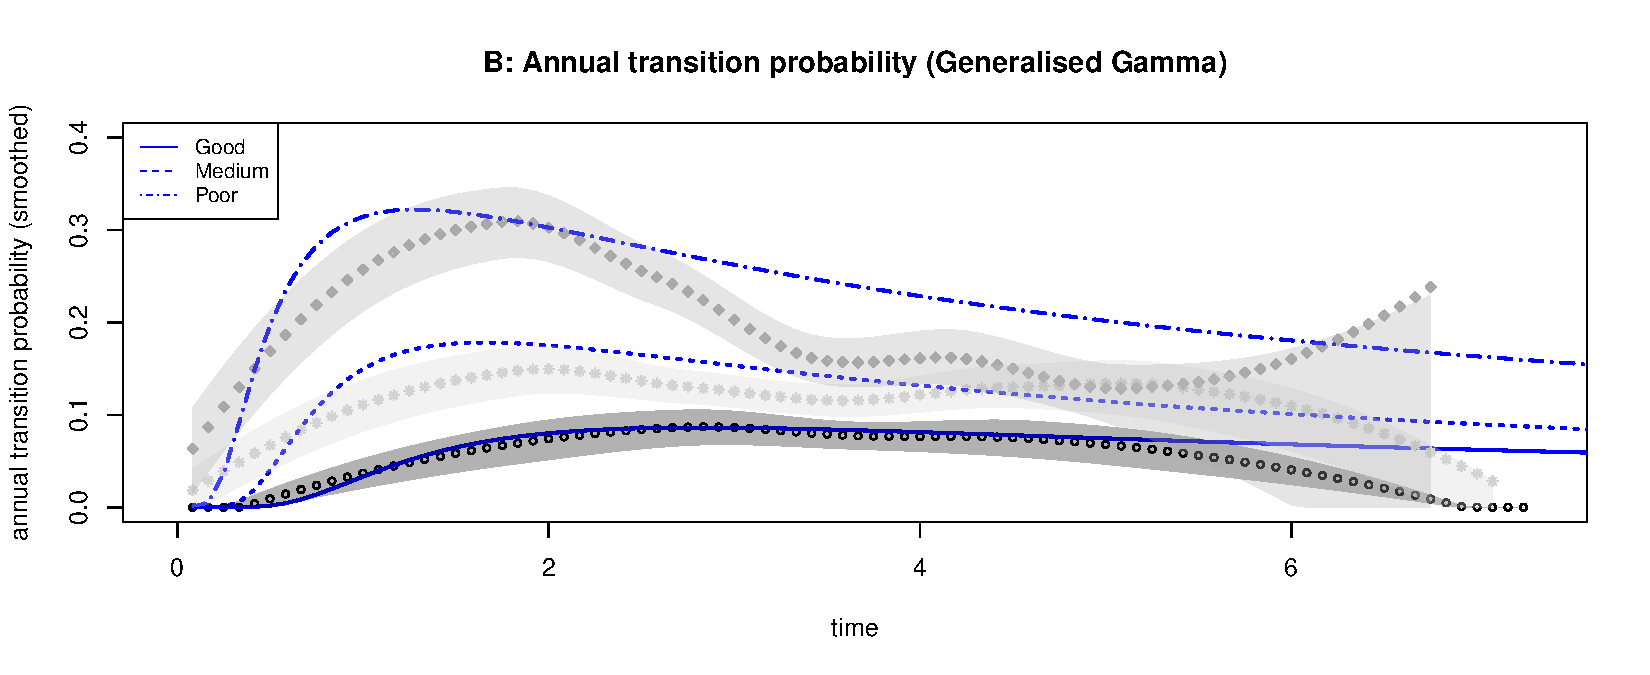
\includegraphics[height=0.3\textheight]{Images/ggam-2} \end{flushleft}

\begin{flushleft}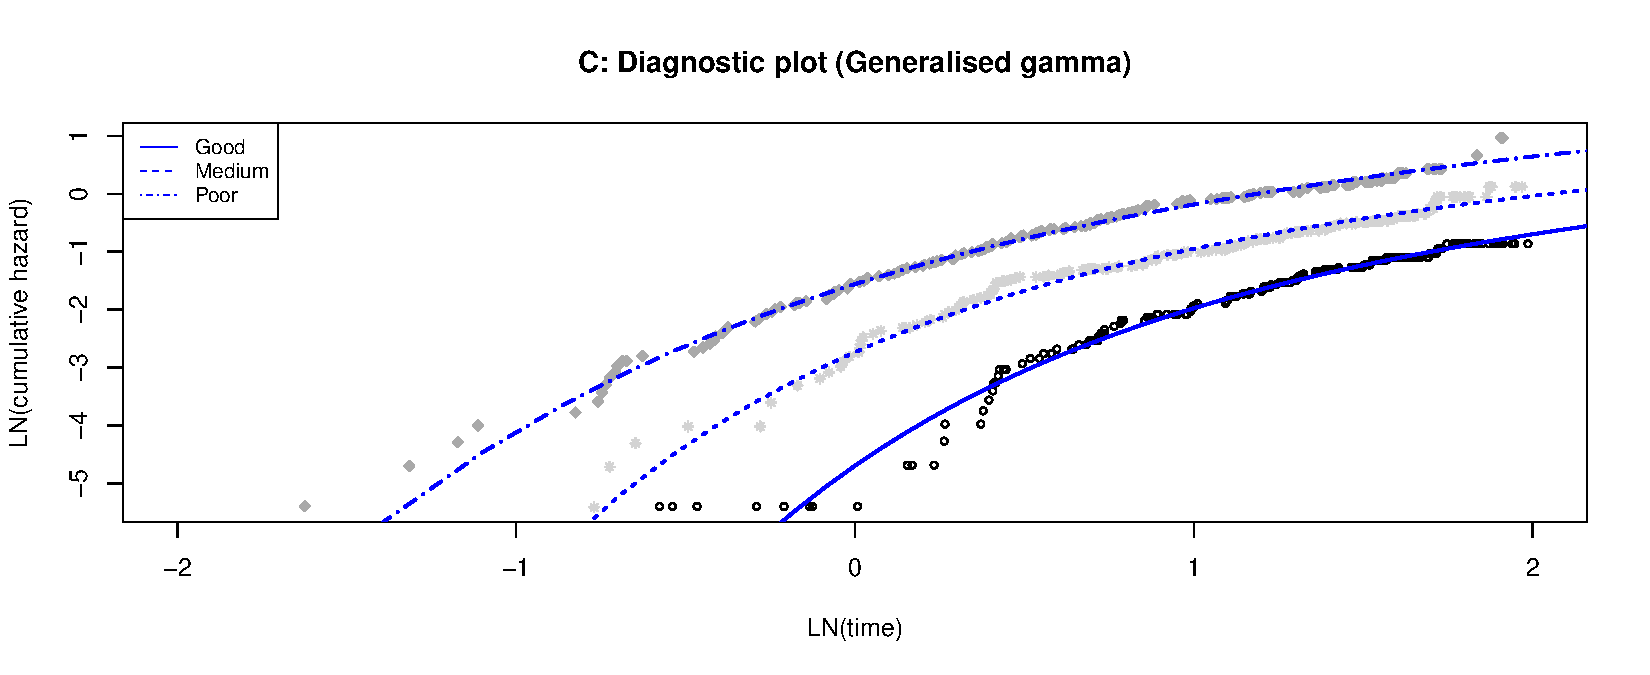
\includegraphics[height=0.3\textheight]{Images/ggam-3} \end{flushleft}

\newpage

\hypertarget{parametric-natural-cubic-spline-models}{%
\section{Parametric natural cubic spline
models?}\label{parametric-natural-cubic-spline-models}}

\hypertarget{if-standard-parametric-models-do-not-provide-a-satisfactory-fit-to-the-data-based-on-previous-observations-do-spline-models-provide-a-more-satisfactory-fit-to-the-data}{%
\subsection{If standard parametric models do not provide a satisfactory
fit to the data based on previous observations, do spline models provide
a more satisfactory fit to the
data?}\label{if-standard-parametric-models-do-not-provide-a-satisfactory-fit-to-the-data-based-on-previous-observations-do-spline-models-provide-a-more-satisfactory-fit-to-the-data}}

An explanation concerning these natural cubic spline models, henceforth
spline models, is provided in
\href{https://doi.org/10.1002/sim.1203}{Royston and Pamar - 2002}.\\
As in the previous section, the circle provides the colours attributed
to each parametric survival model, spline models in this case. The Table
below provides the AIC and BIC for all fitted models. This allows for a
comparison of the fit of the spline models to the `standard' parametric
survival models.\\
\textbf{Interpretation in this case}: Based on this Table, one can
conclude that four spline models fit the data relatively better than the
generalised gamma survival model, due to their lower AIC. The difference
in AIC is however marginal (4 AIC points).\\
\textbf{CAUTION}: These goodness-of-fit statistics only apply to the
observed period of time and do not allow to issue statements about the
suitability of the extrapolated survival by these fitted models beyond
the observation period.

In the following pages, the same three plots per fitted parametric
spline model are displayed to support the visual inspection of the fit
of the models to the observed data, as in previous section. The
interpretation of these plots remains the same.\\
\textbf{Interpretation in this case}: Based on these plots, one can see
that the four spline models fit the data marginally better than the
generalised gamma model.\\
\textbf{CAUTION}: These observations only apply to the observed period
of time and do not allow to issue statements about the suitability of
the extrapolated survival by these fitted models beyond the observation
period. Additionally, the shape of the hazard function (smoothed
transition rates) at the end of the observed period may be affected by
the low number of observations in the tail of the Kaplan-Meier curves.
One should therefore consider these changing hazard at the end of the
observed period cautiously.

\begin{flushleft}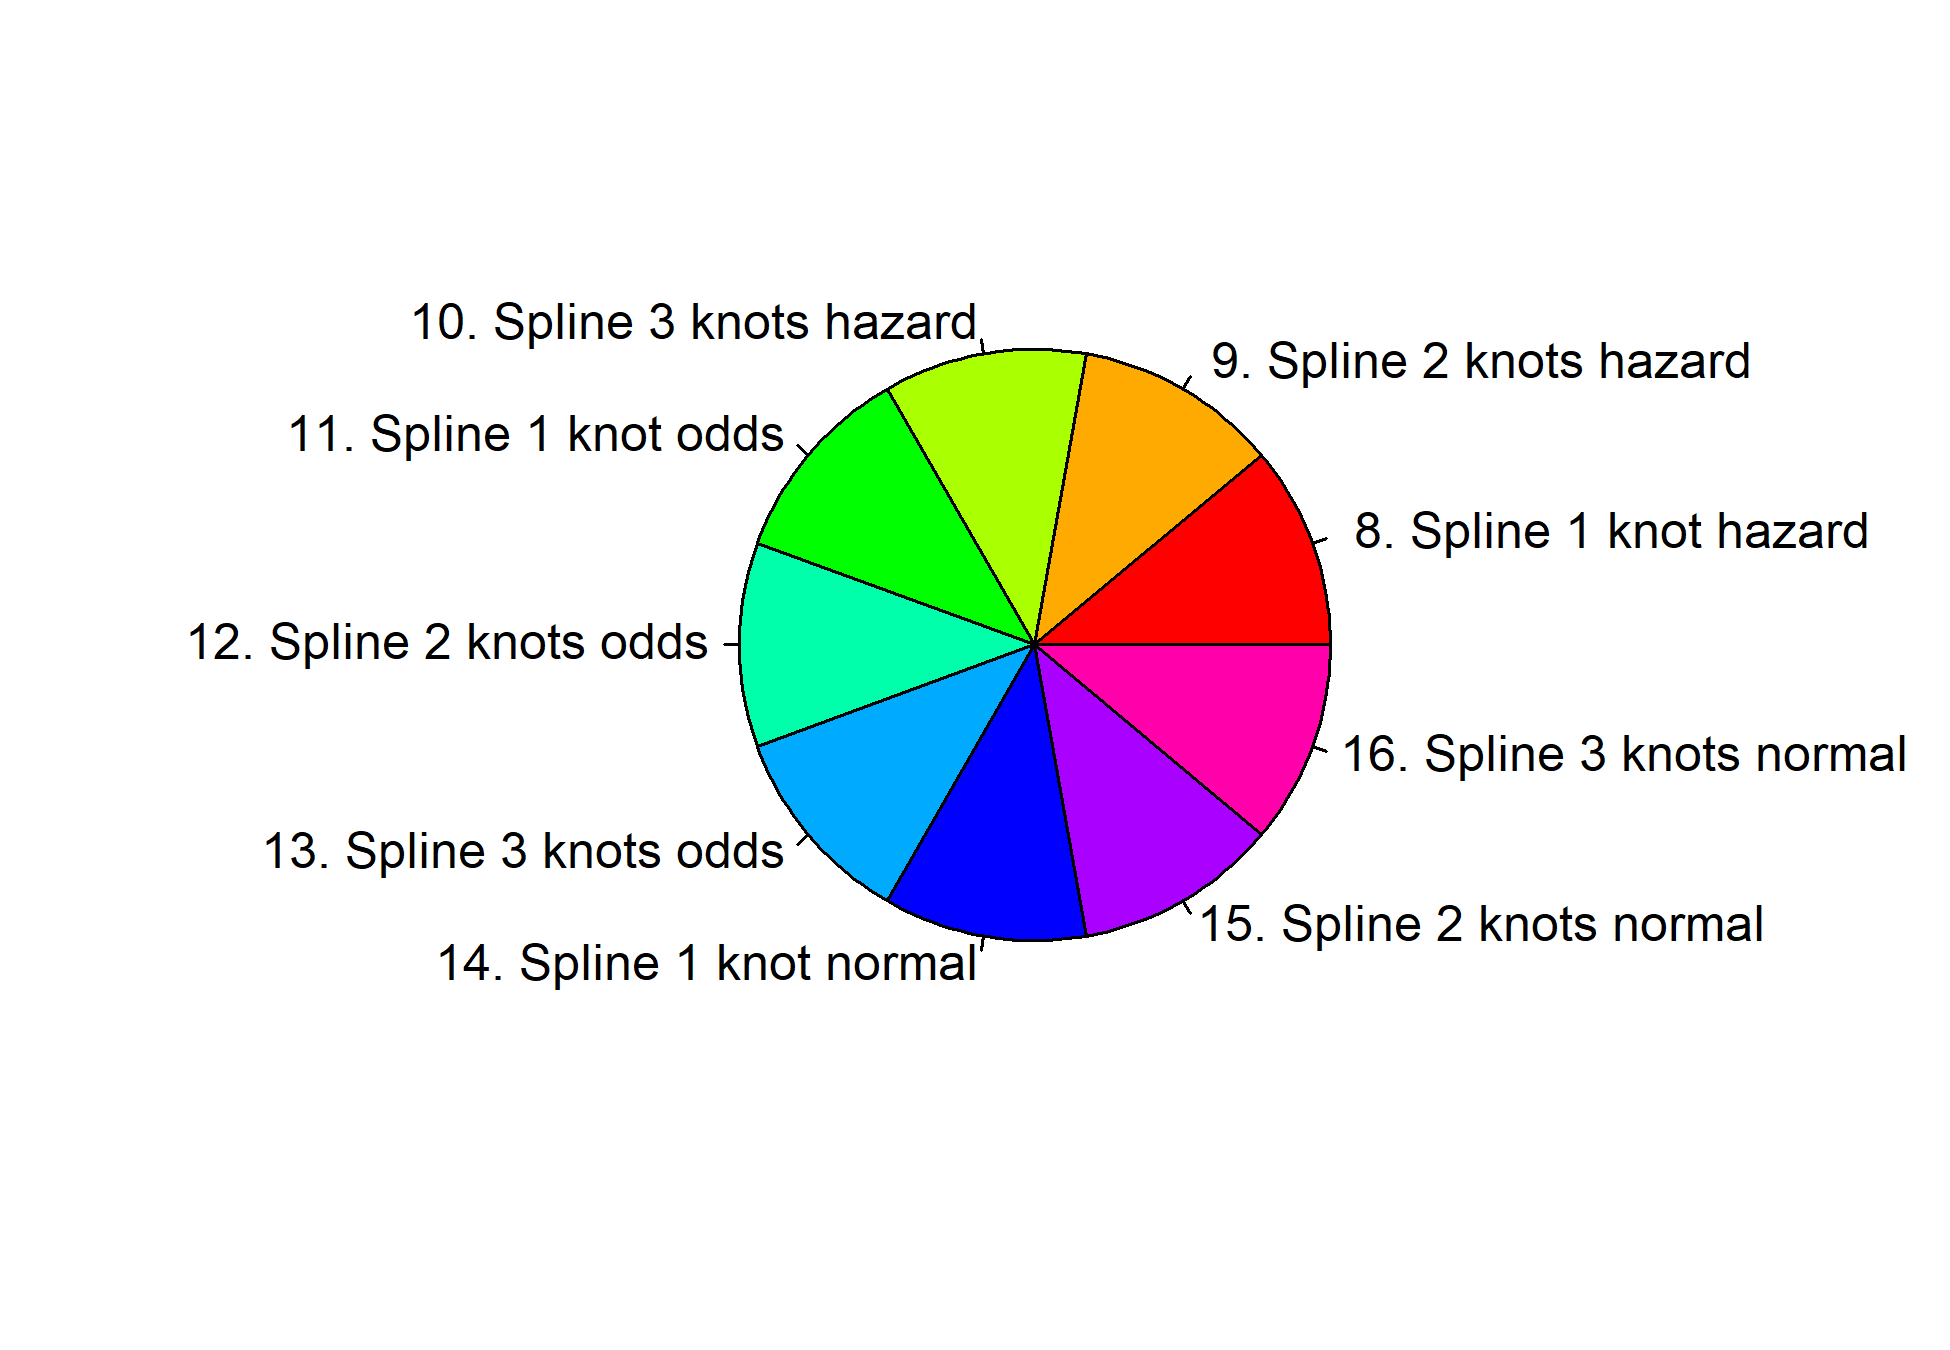
\includegraphics{Images/spline-1} \end{flushleft}

\begin{table}[H]
\centering
\begin{tabular}{lrr}
\toprule
Model & AIC & BIC\\
\midrule
\cellcolor{gray!6}{9. Spline 2 knots hazard} & \cellcolor{gray!6}{1585.894} & \cellcolor{gray!6}{1640.264}\\
12. Spline 2 knots odds & 1587.289 & 1641.659\\
\cellcolor{gray!6}{14. Spline 1 knot normal} & \cellcolor{gray!6}{1587.682} & \cellcolor{gray!6}{1628.460}\\
15. Spline 2 knots normal & 1588.343 & 1642.714\\
\cellcolor{gray!6}{7. Generalised Gamma} & \cellcolor{gray!6}{1589.049} & \cellcolor{gray!6}{1629.826}\\
8. Spline 1 knot hazard & 1589.327 & 1630.105\\
\cellcolor{gray!6}{16. Spline 3 knots normal} & \cellcolor{gray!6}{1589.832} & \cellcolor{gray!6}{1657.795}\\
10. Spline 3 knots hazard & 1589.875 & 1657.838\\
\cellcolor{gray!6}{11. Spline 1 knot odds} & \cellcolor{gray!6}{1590.221} & \cellcolor{gray!6}{1630.999}\\
13. Spline 3 knots odds & 1590.720 & 1658.683\\
\cellcolor{gray!6}{4. Log-normal} & \cellcolor{gray!6}{1592.880} & \cellcolor{gray!6}{1620.066}\\
5. Log-logistic & 1609.294 & 1636.479\\
\cellcolor{gray!6}{6. Gamma} & \cellcolor{gray!6}{1621.982} & \cellcolor{gray!6}{1649.167}\\
2. Weibull & 1632.618 & 1659.803\\
\cellcolor{gray!6}{3. Gompertz} & \cellcolor{gray!6}{1660.954} & \cellcolor{gray!6}{1688.140}\\
1. Exponential & 1668.212 & 1681.805\\
\bottomrule
\end{tabular}
\end{table}

\hypertarget{spline-hazard-1-knot}{%
\subsection{Spline hazard 1 knot}\label{spline-hazard-1-knot}}

\begin{flushleft}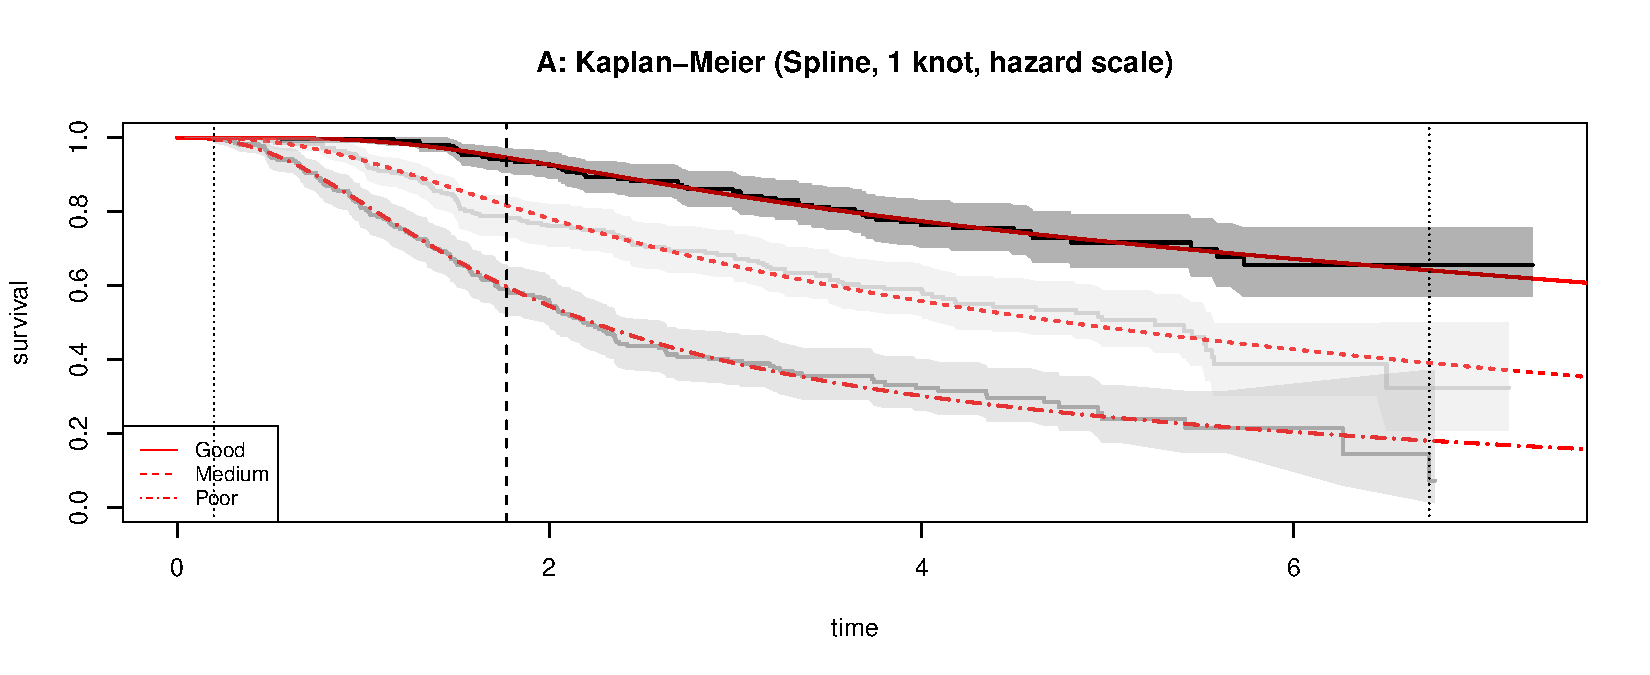
\includegraphics[height=0.3\textheight]{Images/spline_hazard1-1} \end{flushleft}

\begin{flushleft}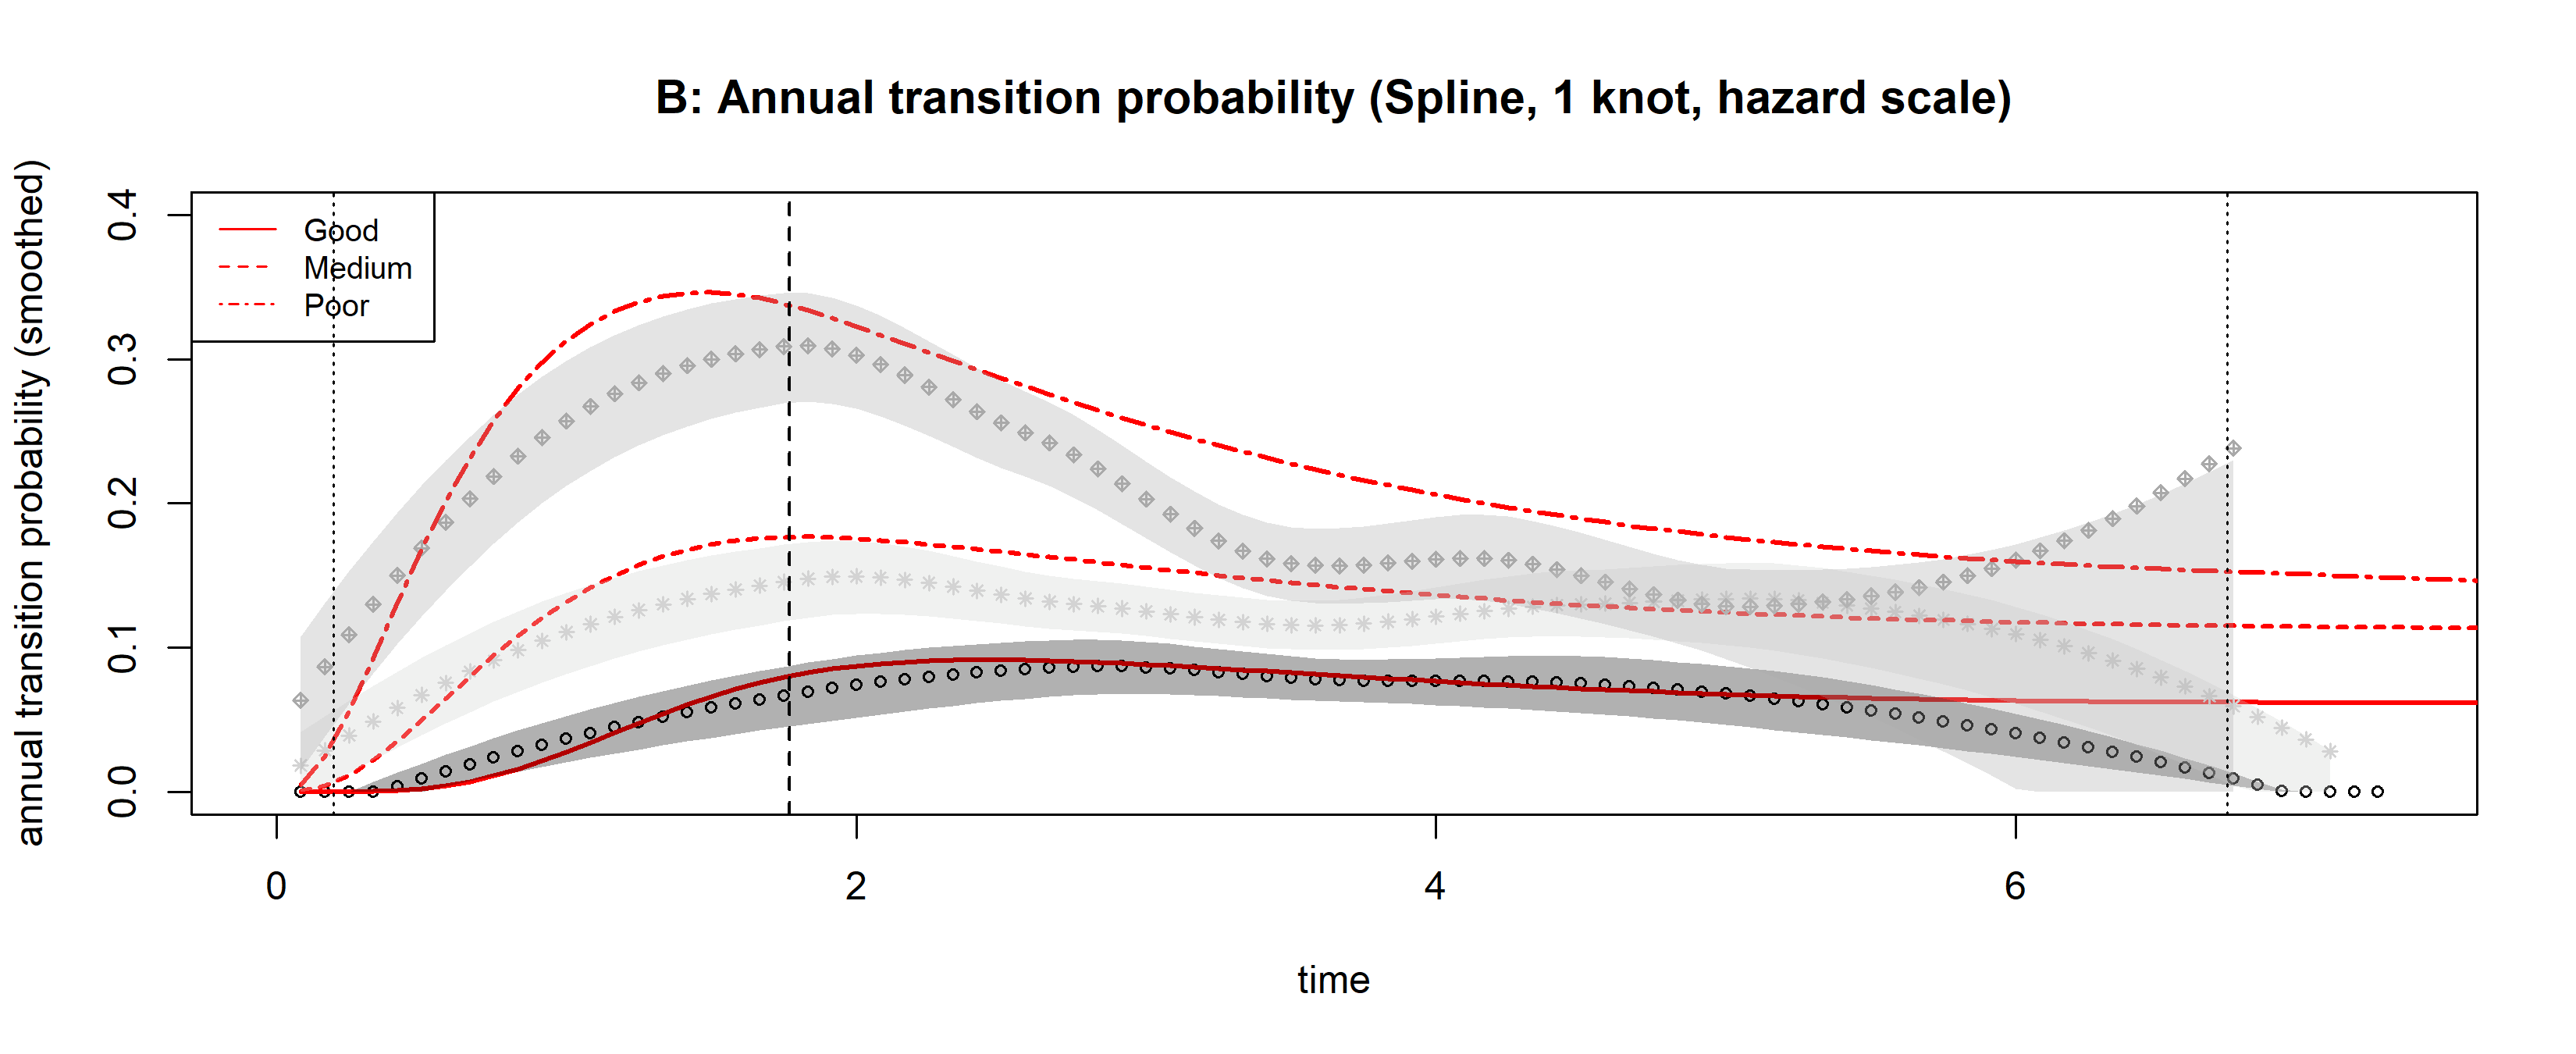
\includegraphics[height=0.3\textheight]{Images/spline_hazard1-2} \end{flushleft}

\begin{flushleft}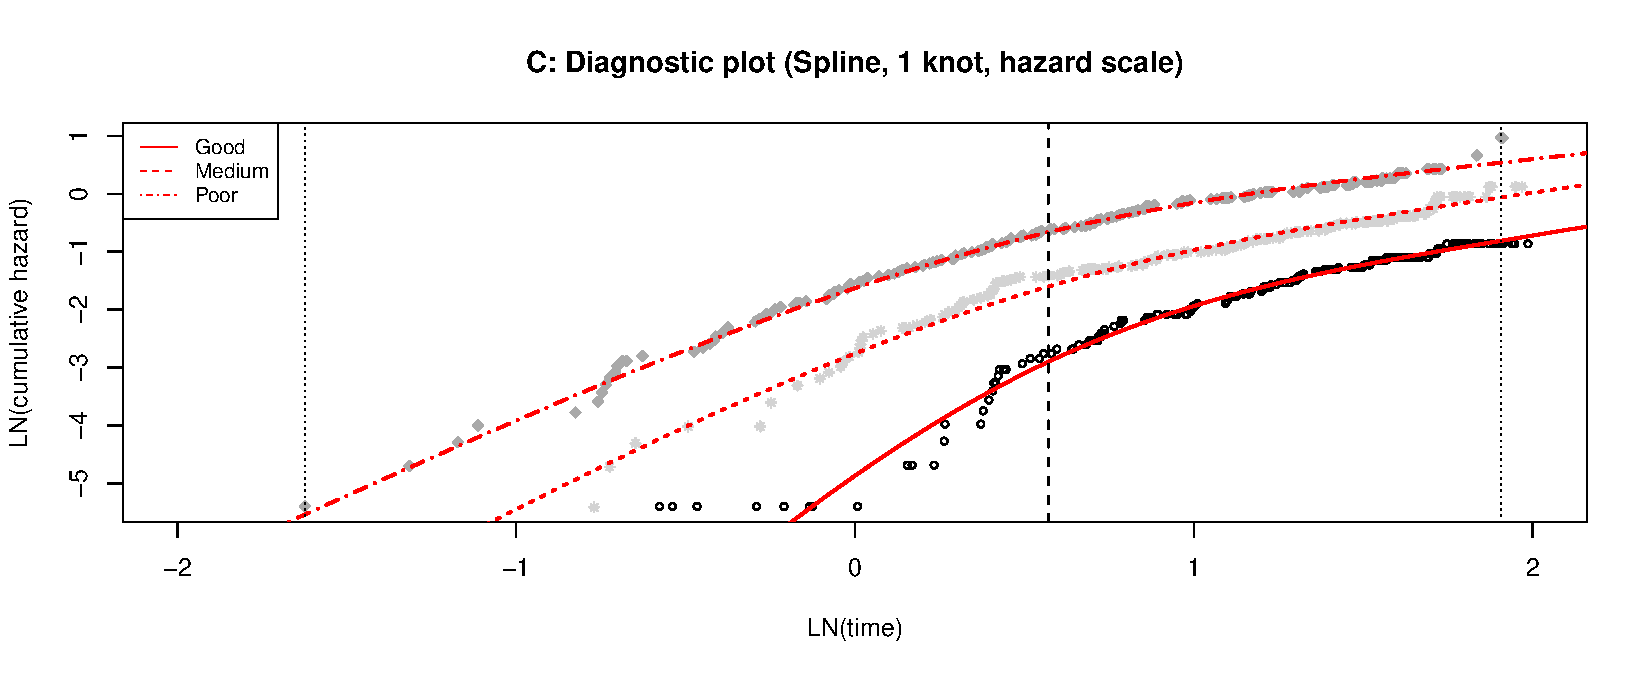
\includegraphics[height=0.3\textheight]{Images/spline_hazard1-3} \end{flushleft}

\hypertarget{spline-hazard-2-knots}{%
\subsection{Spline hazard 2 knots}\label{spline-hazard-2-knots}}

\begin{flushleft}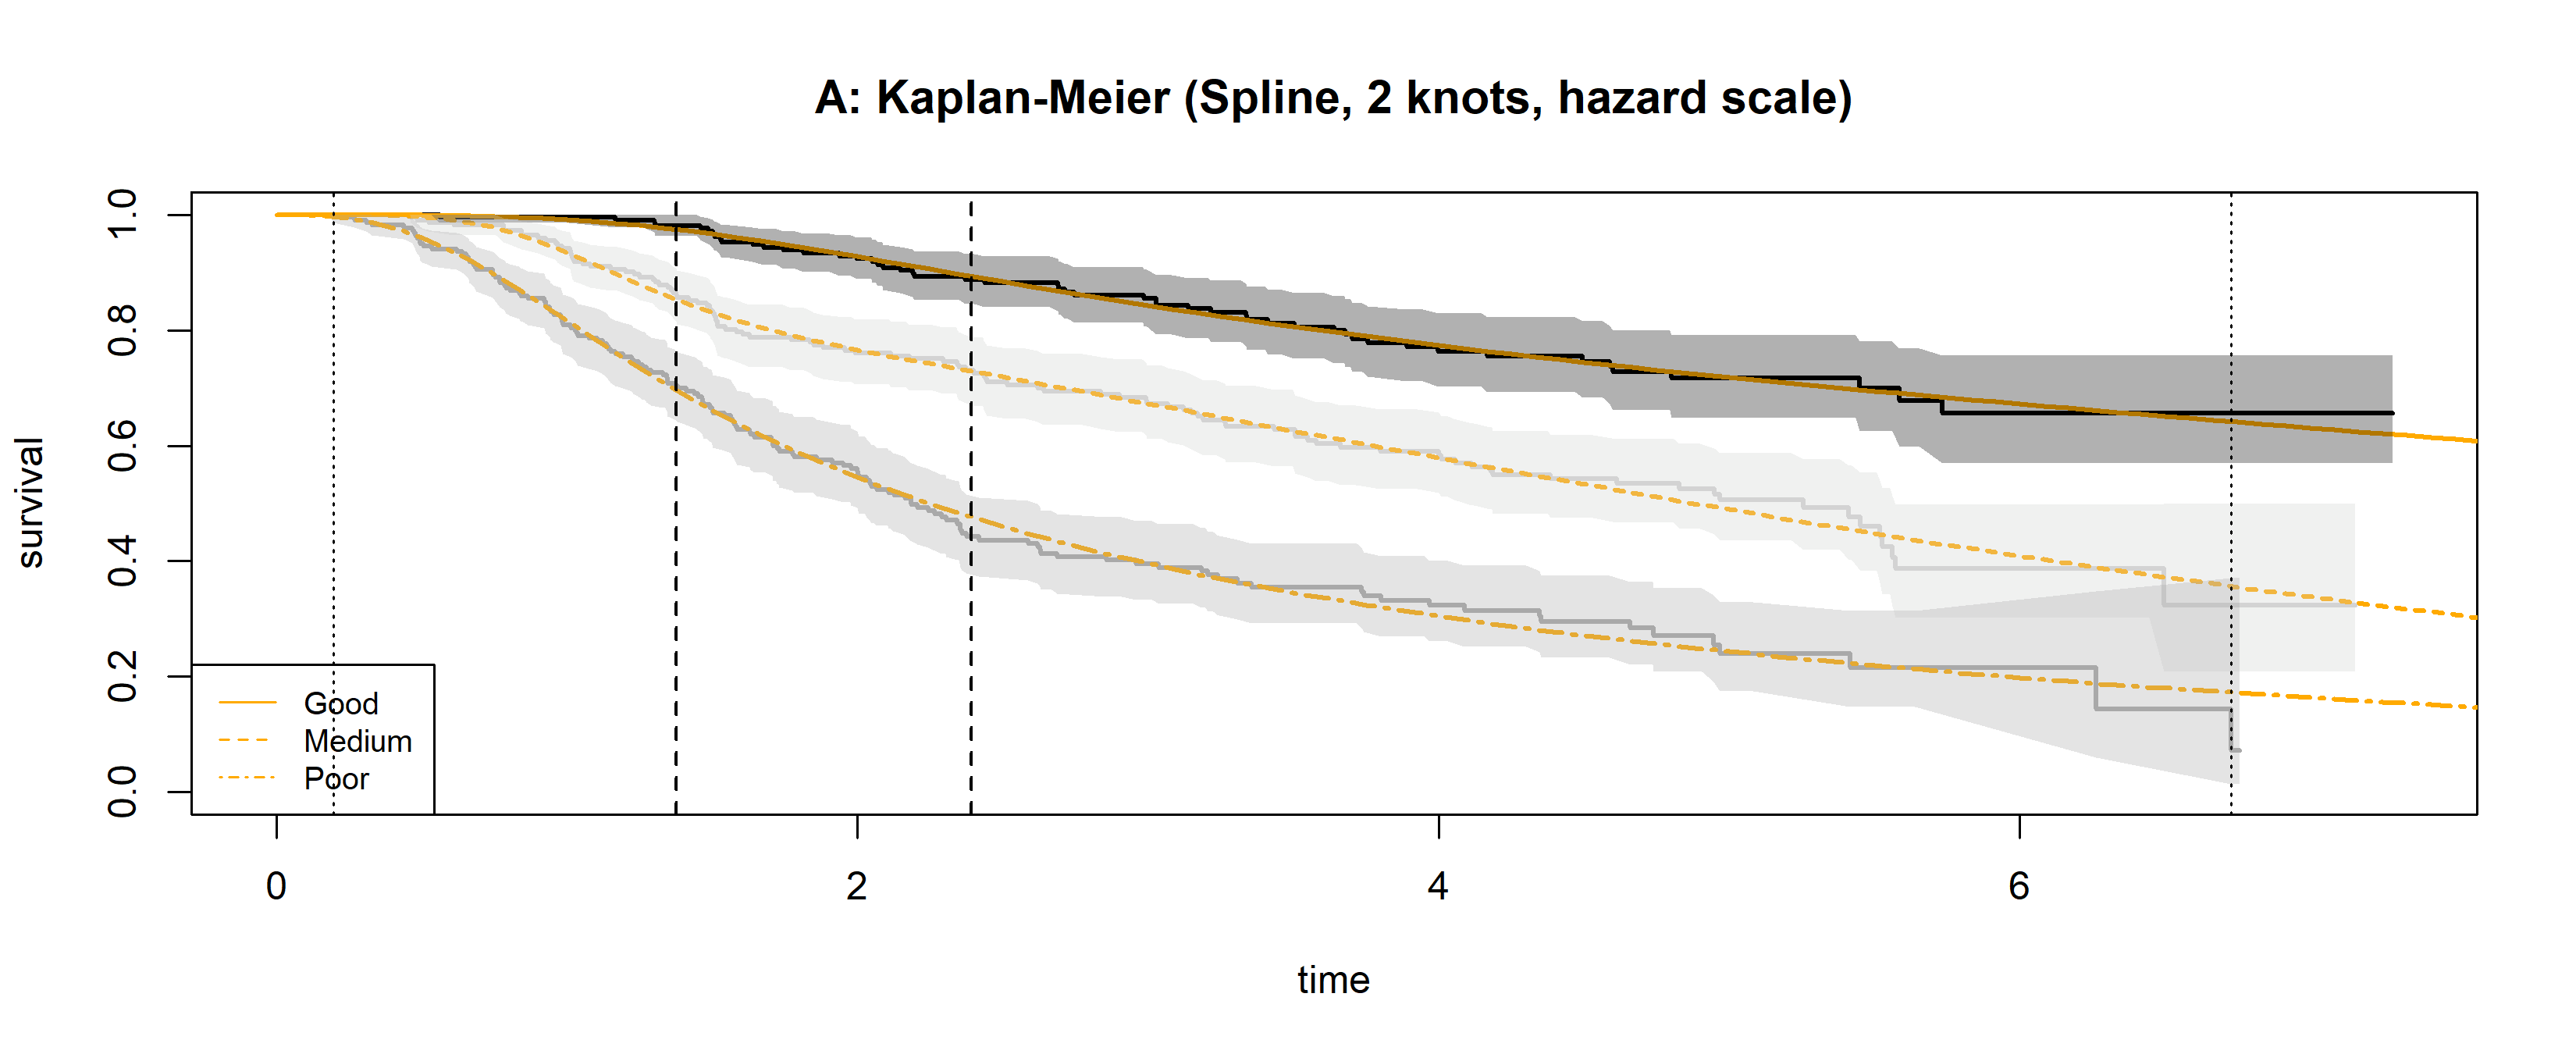
\includegraphics[height=0.3\textheight]{Images/spline_hazard2-1} \end{flushleft}

\begin{flushleft}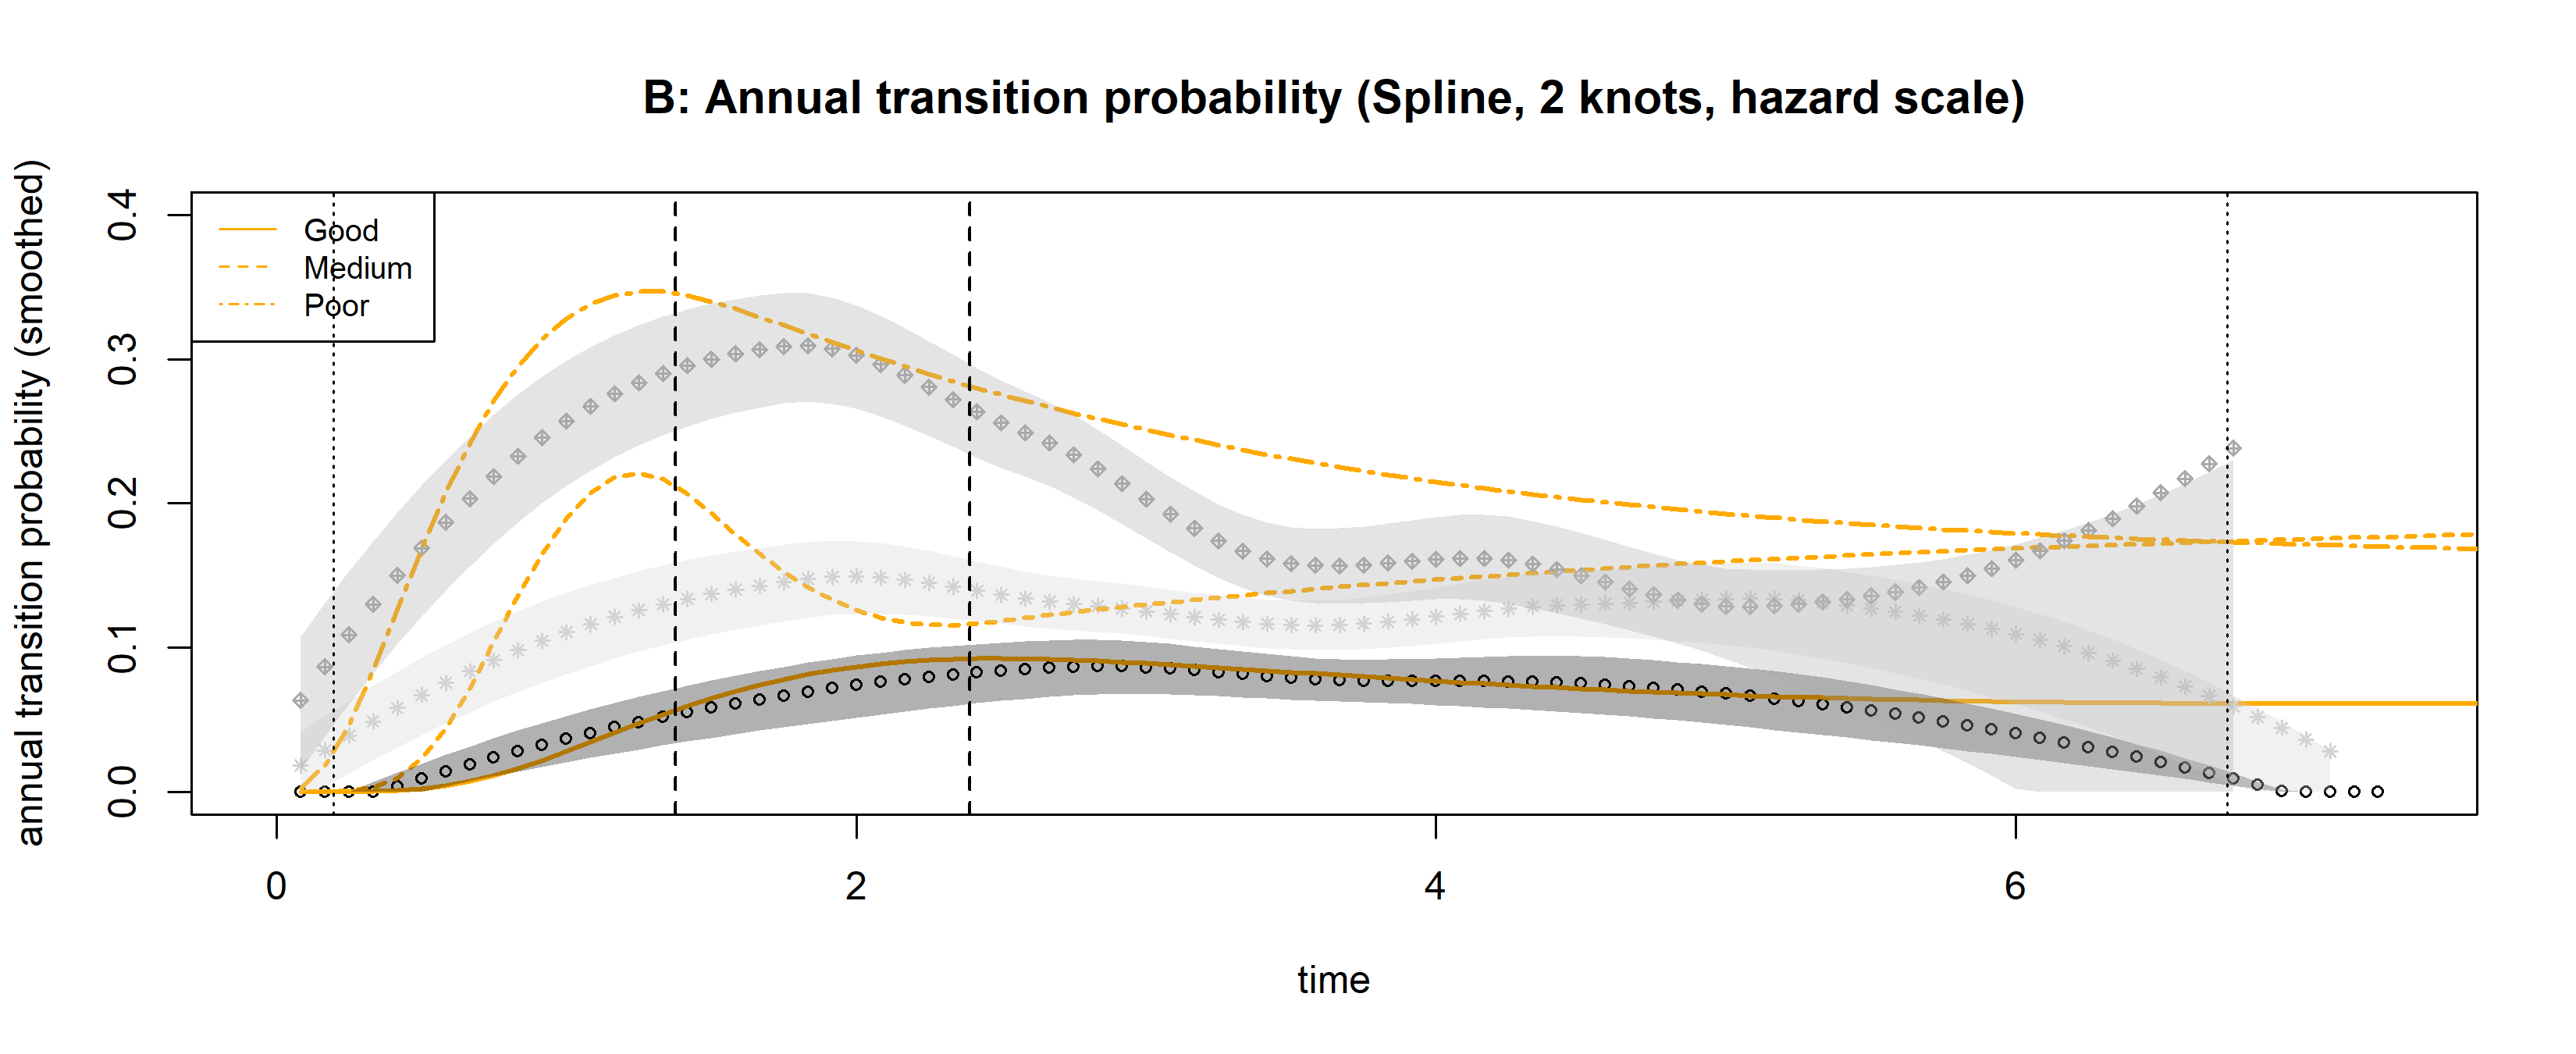
\includegraphics[height=0.3\textheight]{Images/spline_hazard2-2} \end{flushleft}

\begin{flushleft}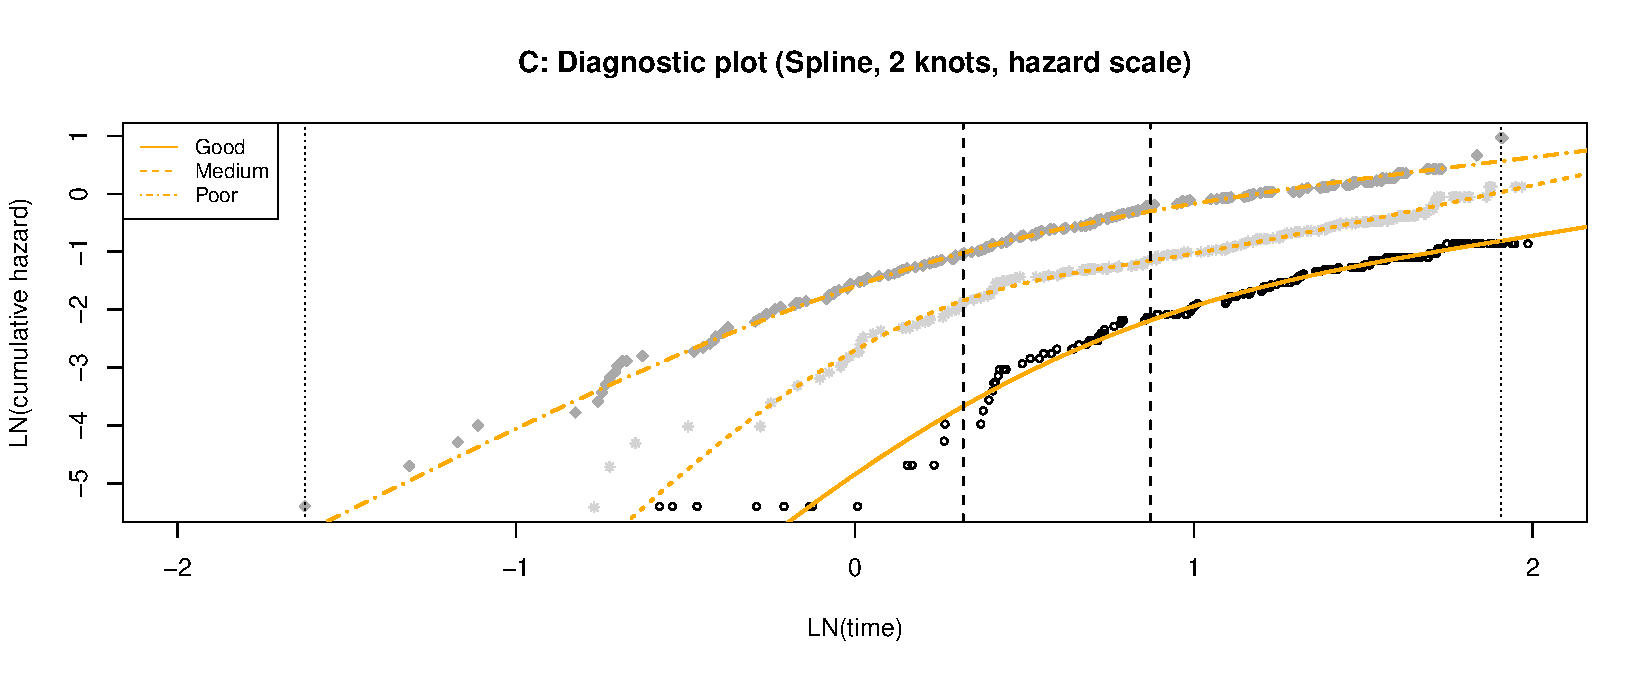
\includegraphics[height=0.3\textheight]{Images/spline_hazard2-3} \end{flushleft}

\hypertarget{spline-hazard-3-knots}{%
\subsection{Spline hazard 3 knots}\label{spline-hazard-3-knots}}

\begin{flushleft}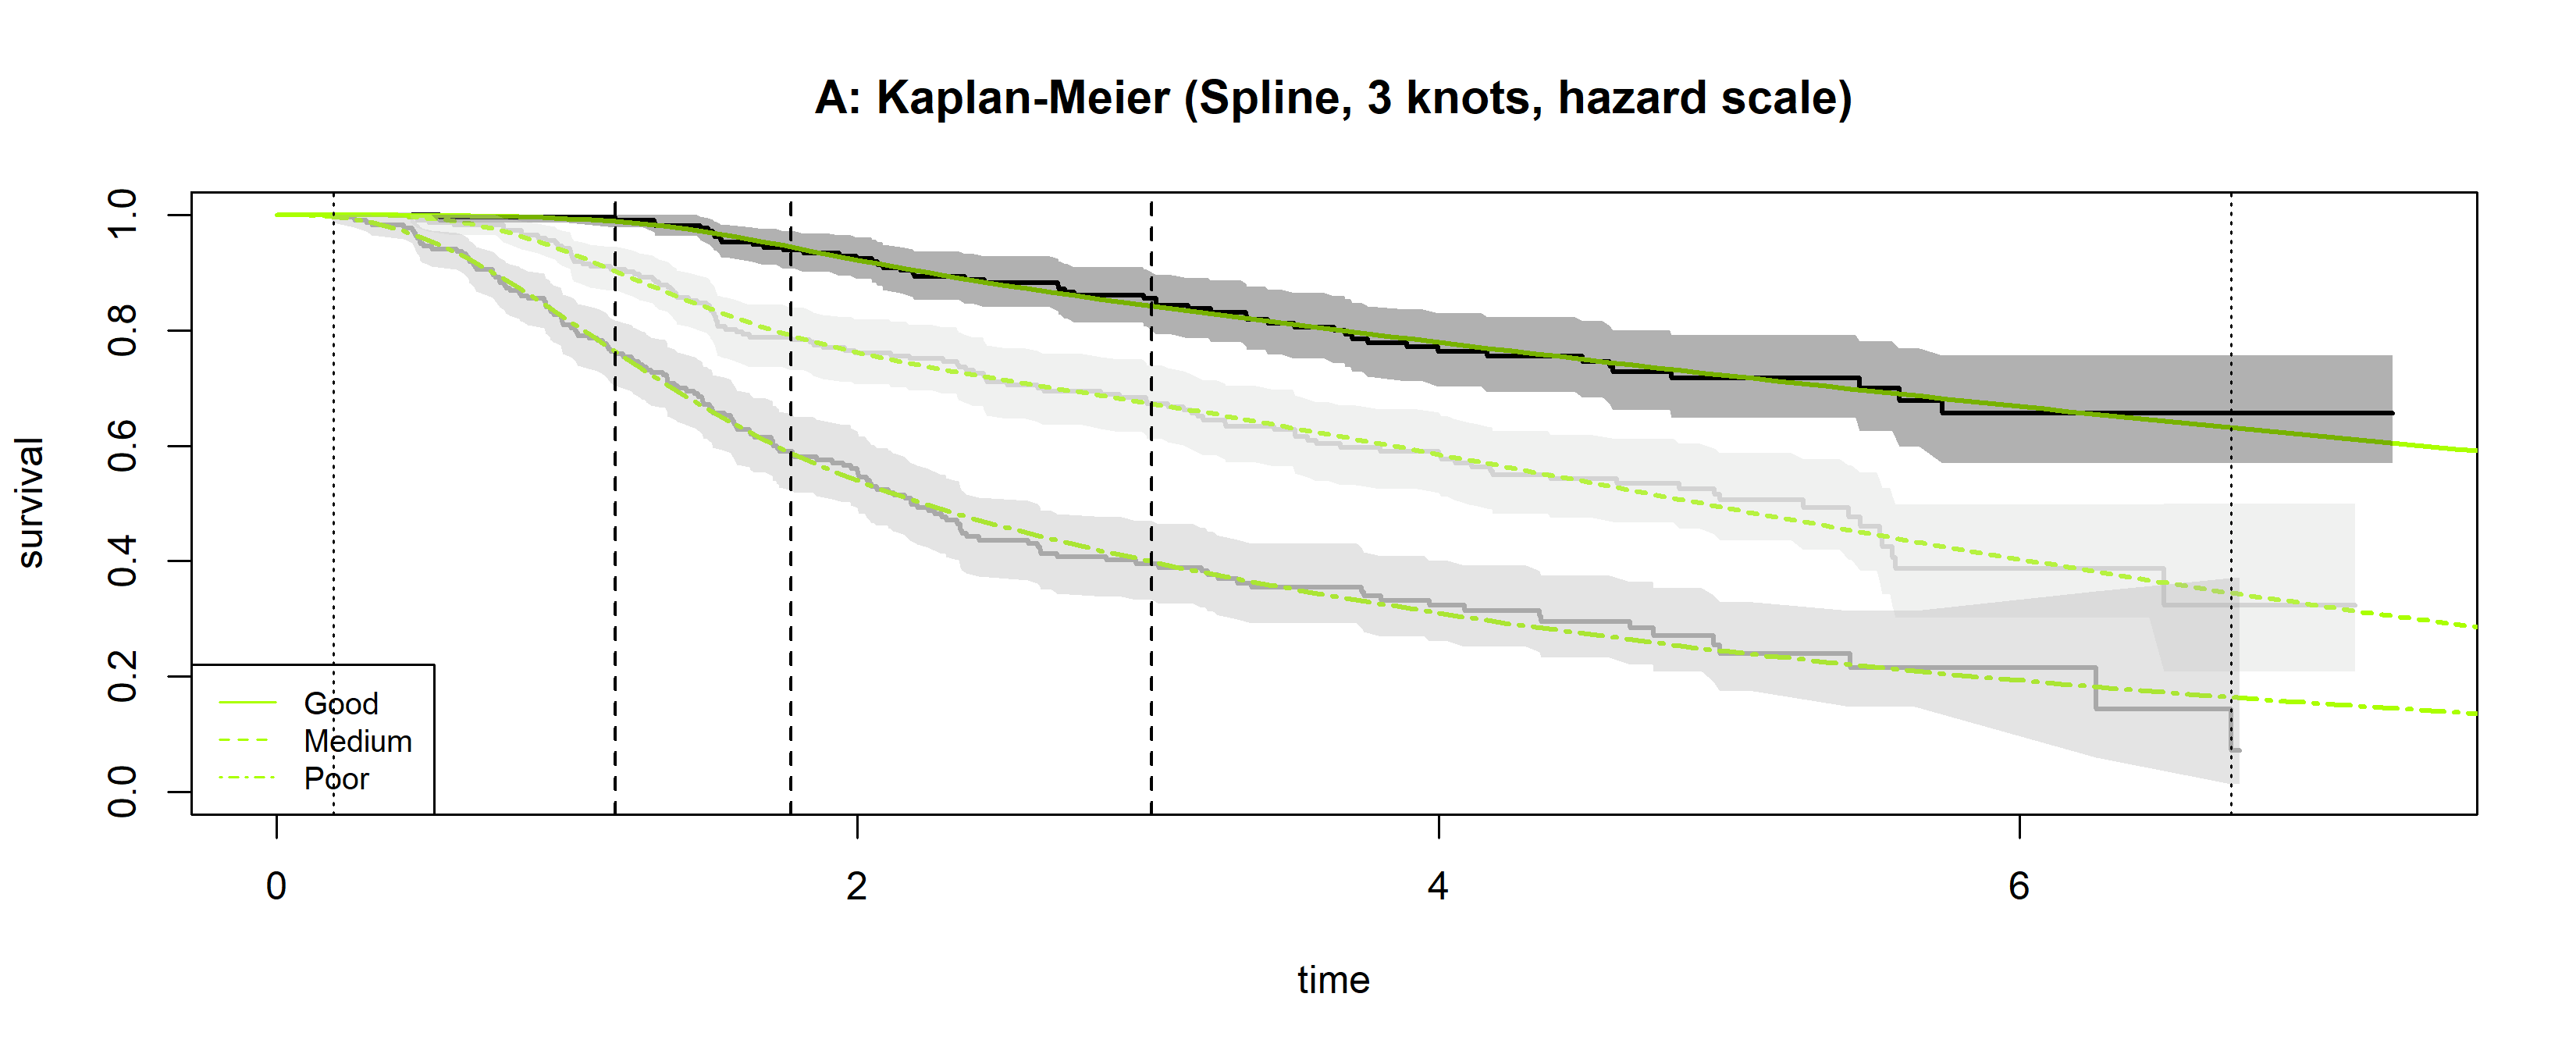
\includegraphics[height=0.3\textheight]{Images/spline_hazard3-1} \end{flushleft}

\begin{flushleft}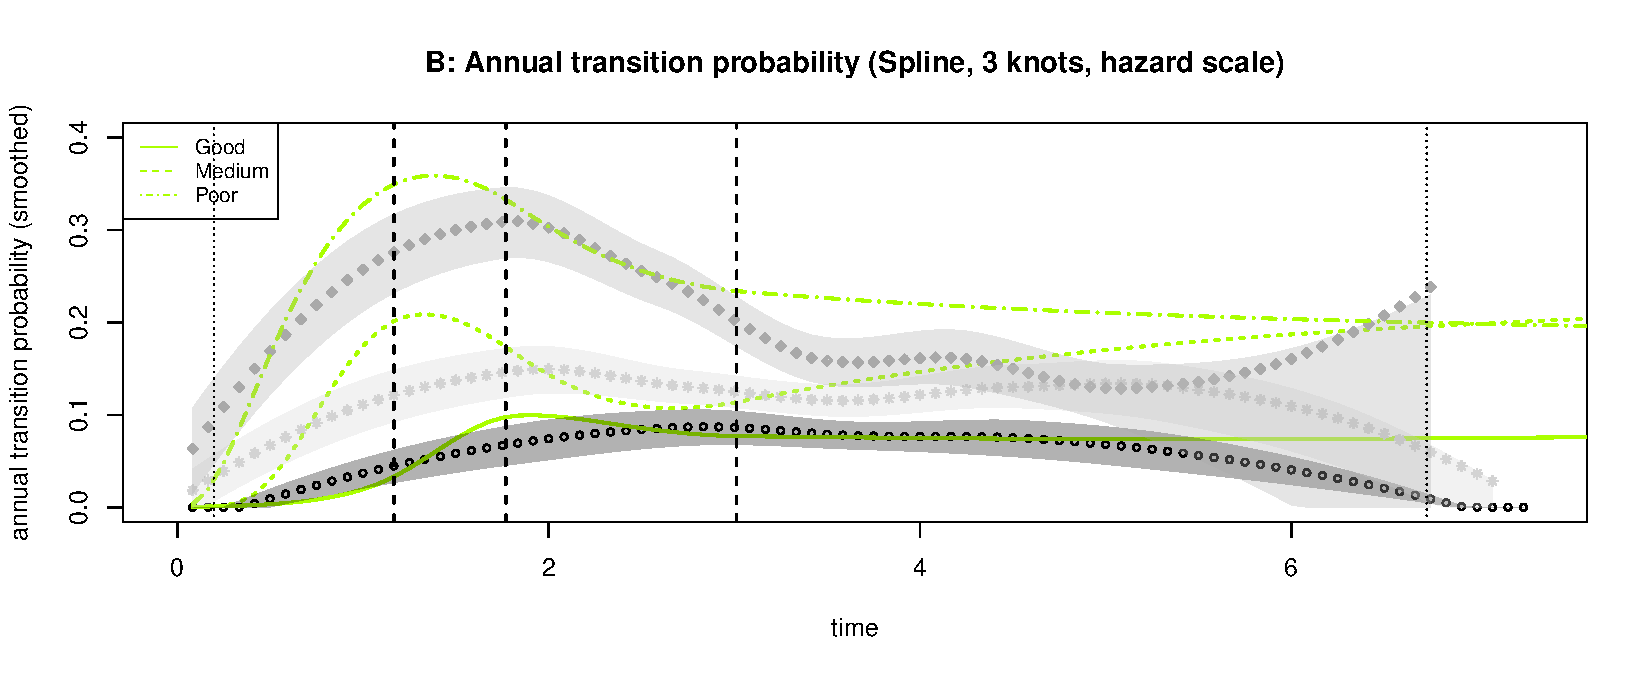
\includegraphics[height=0.3\textheight]{Images/spline_hazard3-2} \end{flushleft}

\begin{flushleft}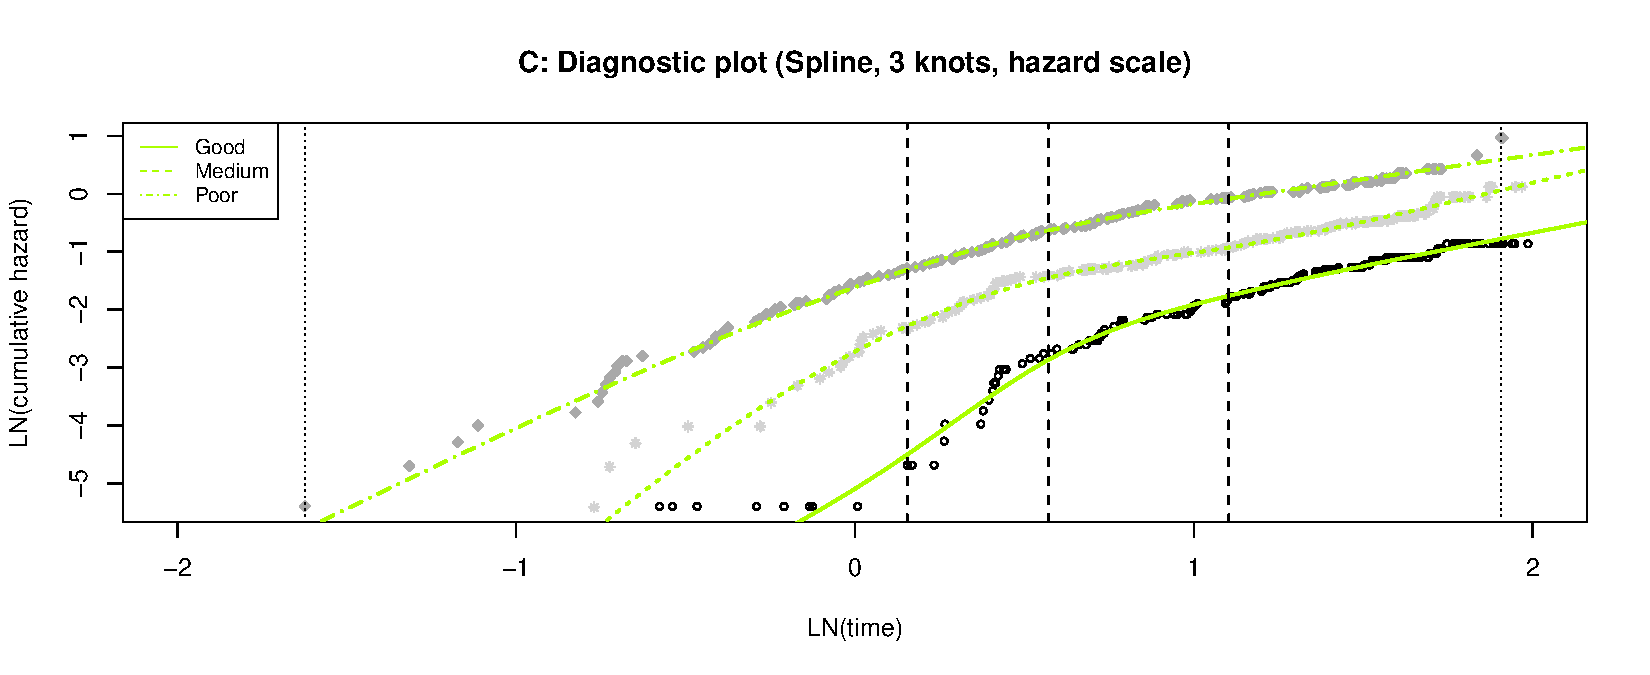
\includegraphics[height=0.3\textheight]{Images/spline_hazard3-3} \end{flushleft}

\hypertarget{spline-odds-1-knot}{%
\subsection{Spline odds 1 knot}\label{spline-odds-1-knot}}

\begin{flushleft}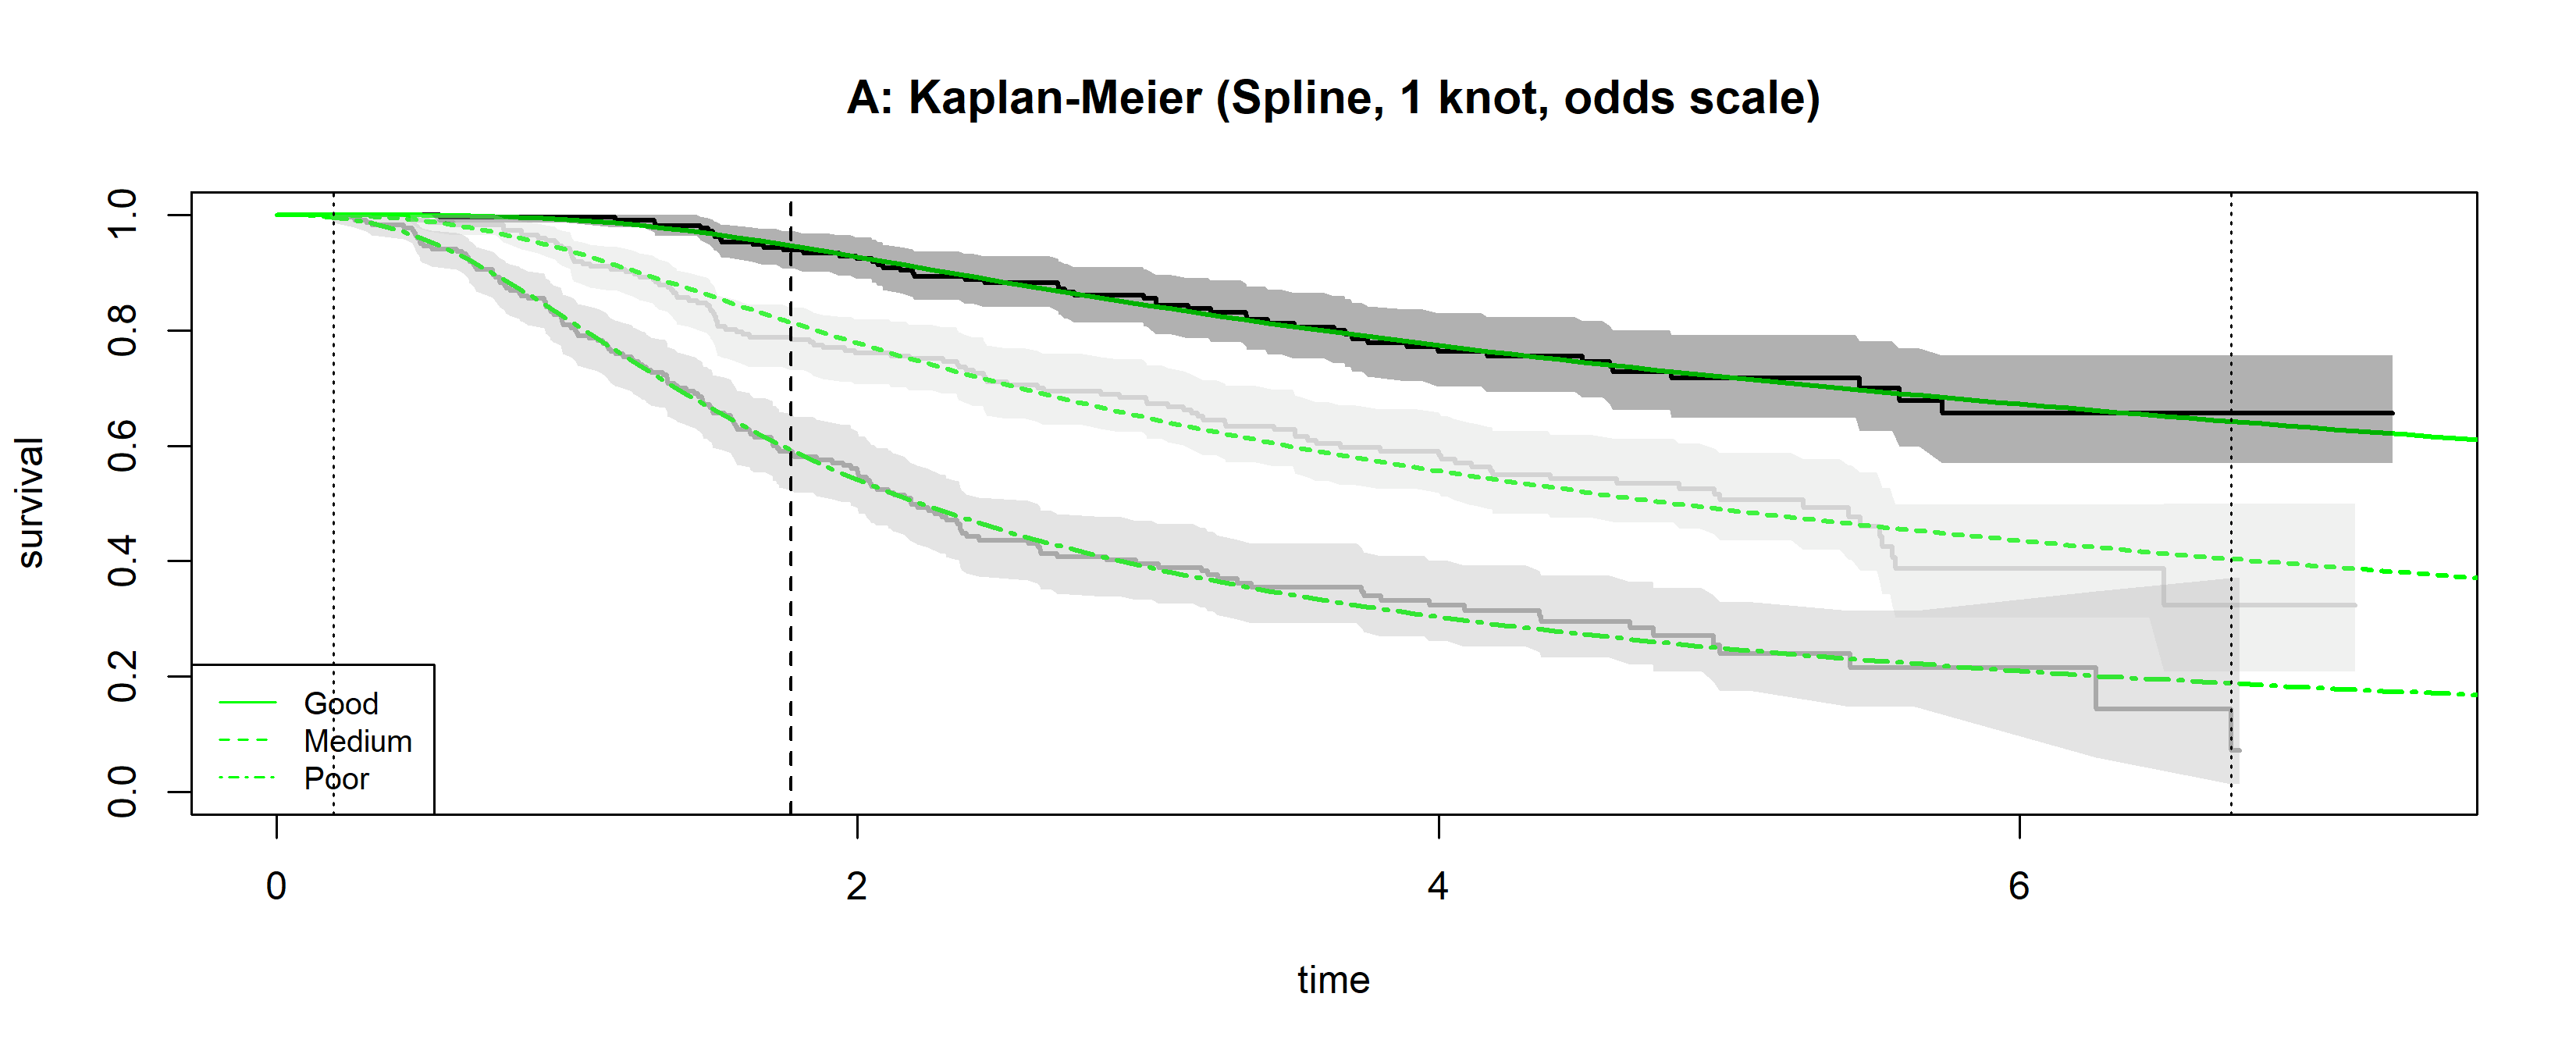
\includegraphics[height=0.3\textheight]{Images/spline_odds1-1} \end{flushleft}

\begin{flushleft}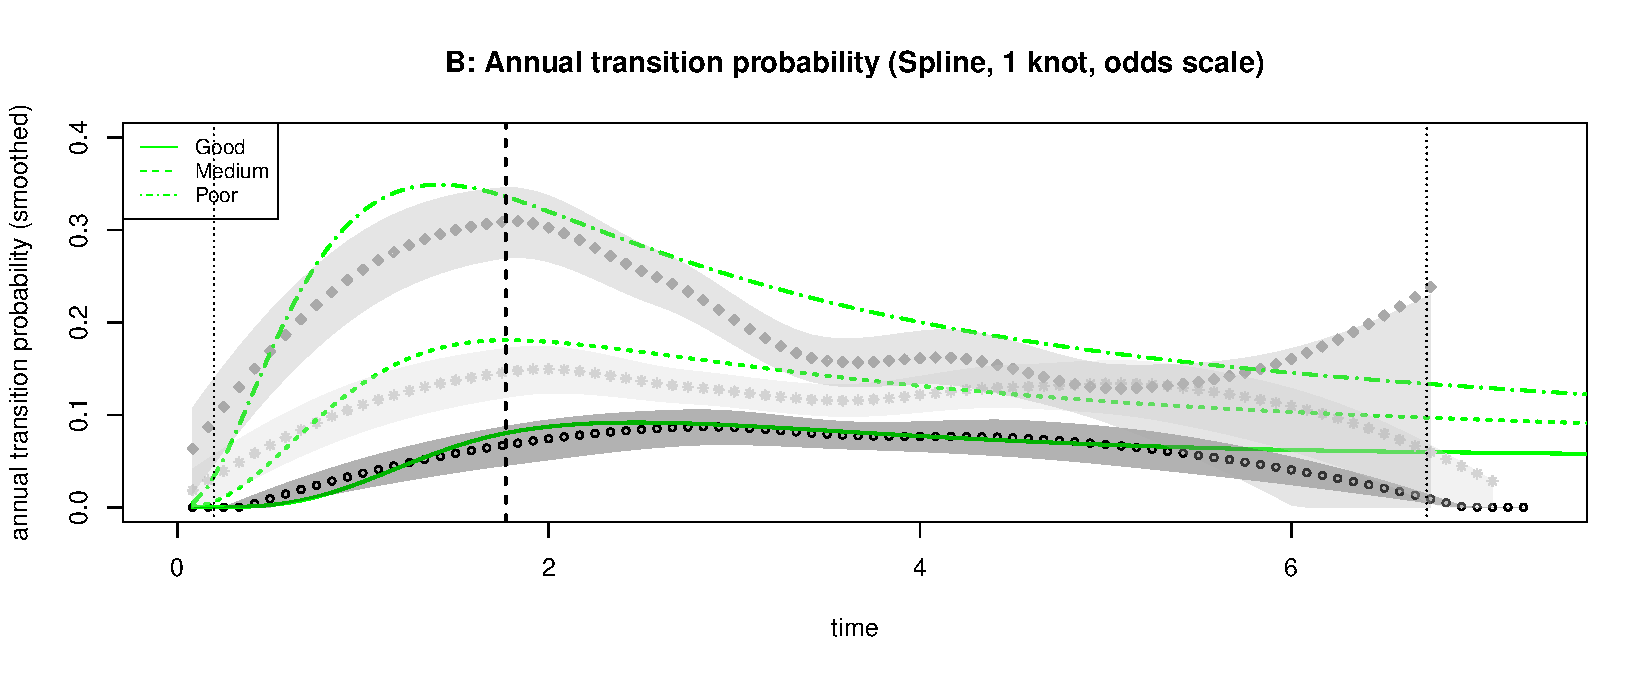
\includegraphics[height=0.3\textheight]{Images/spline_odds1-2} \end{flushleft}

\begin{flushleft}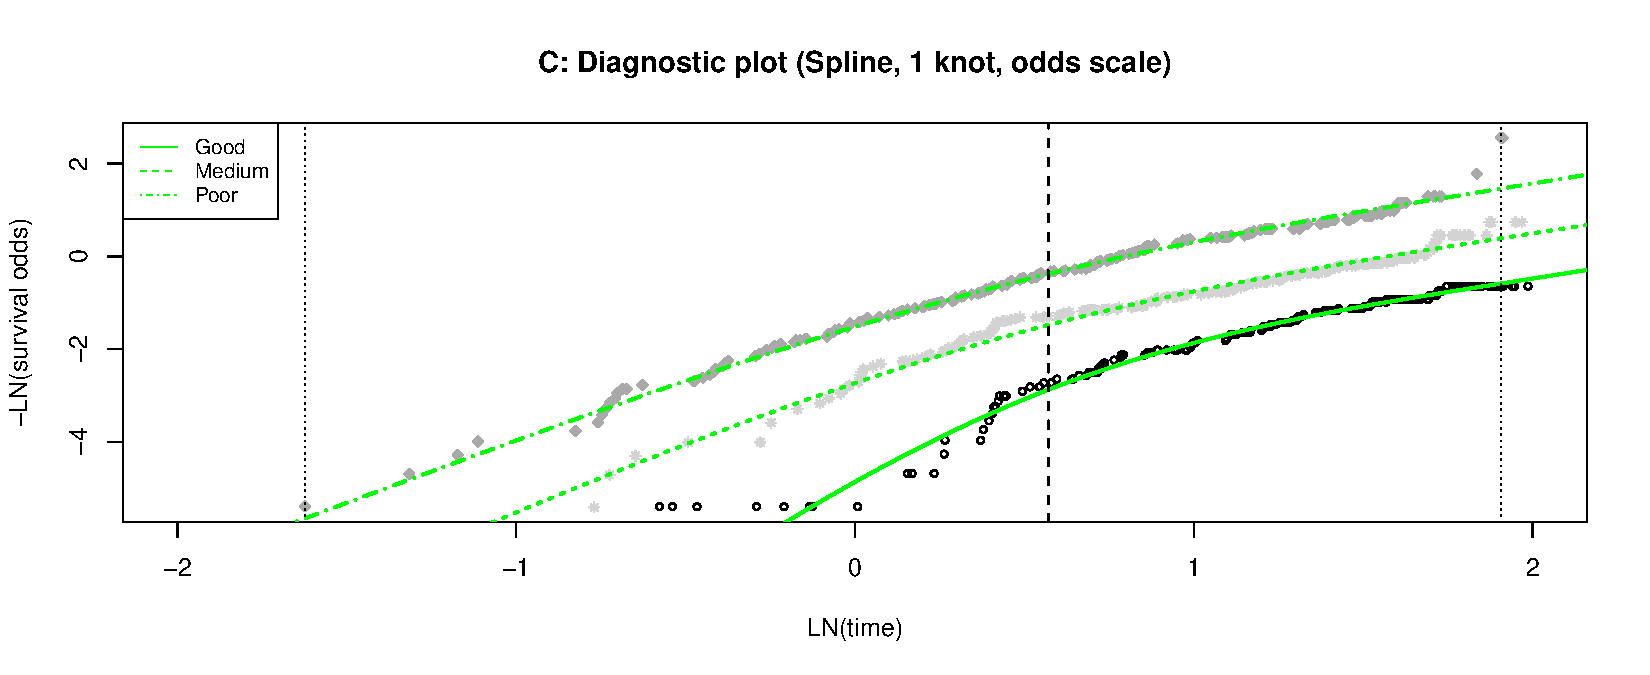
\includegraphics[height=0.3\textheight]{Images/spline_odds1-3} \end{flushleft}

\hypertarget{spline-odds-2-knots}{%
\subsection{Spline odds 2 knots}\label{spline-odds-2-knots}}

\begin{flushleft}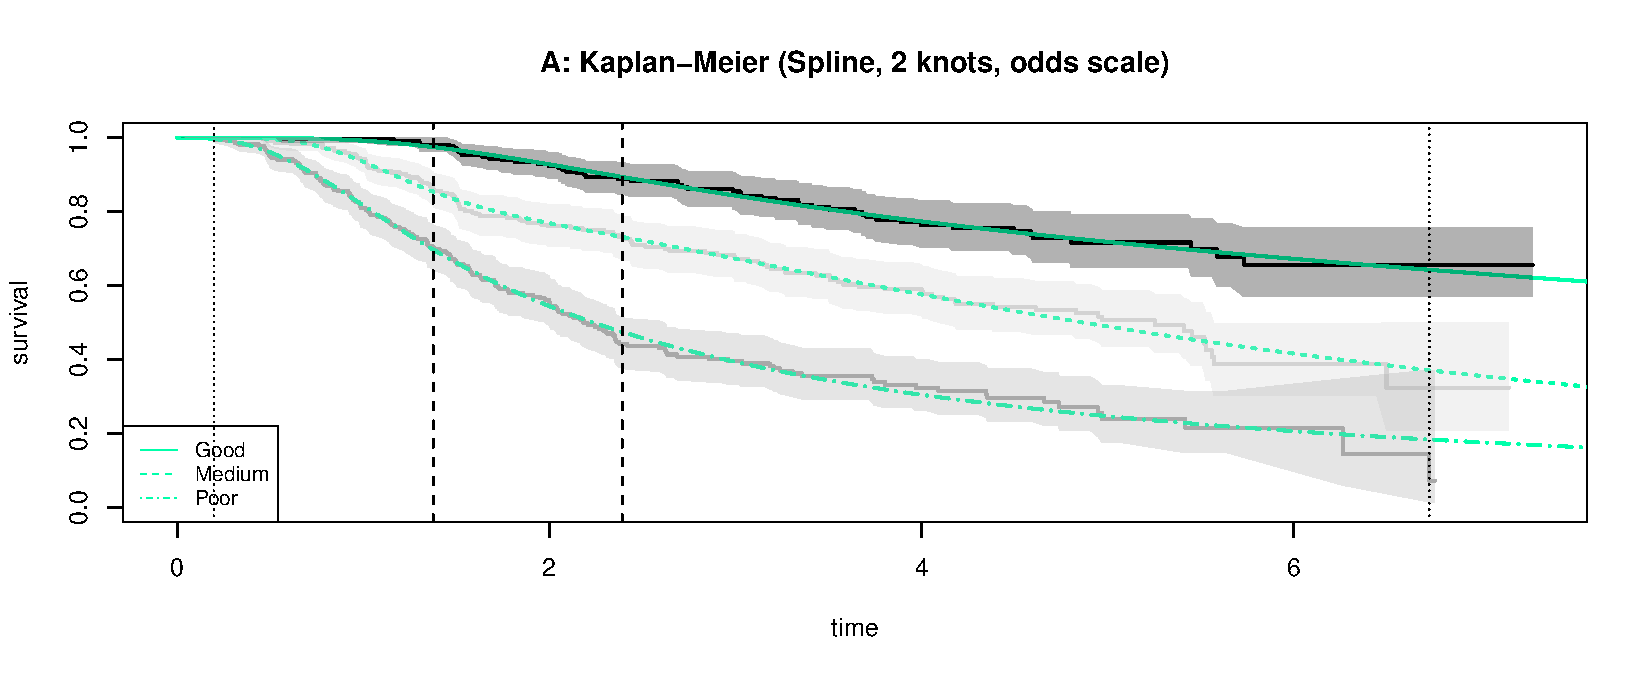
\includegraphics[height=0.3\textheight]{Images/spline_odds2-1} \end{flushleft}

\begin{flushleft}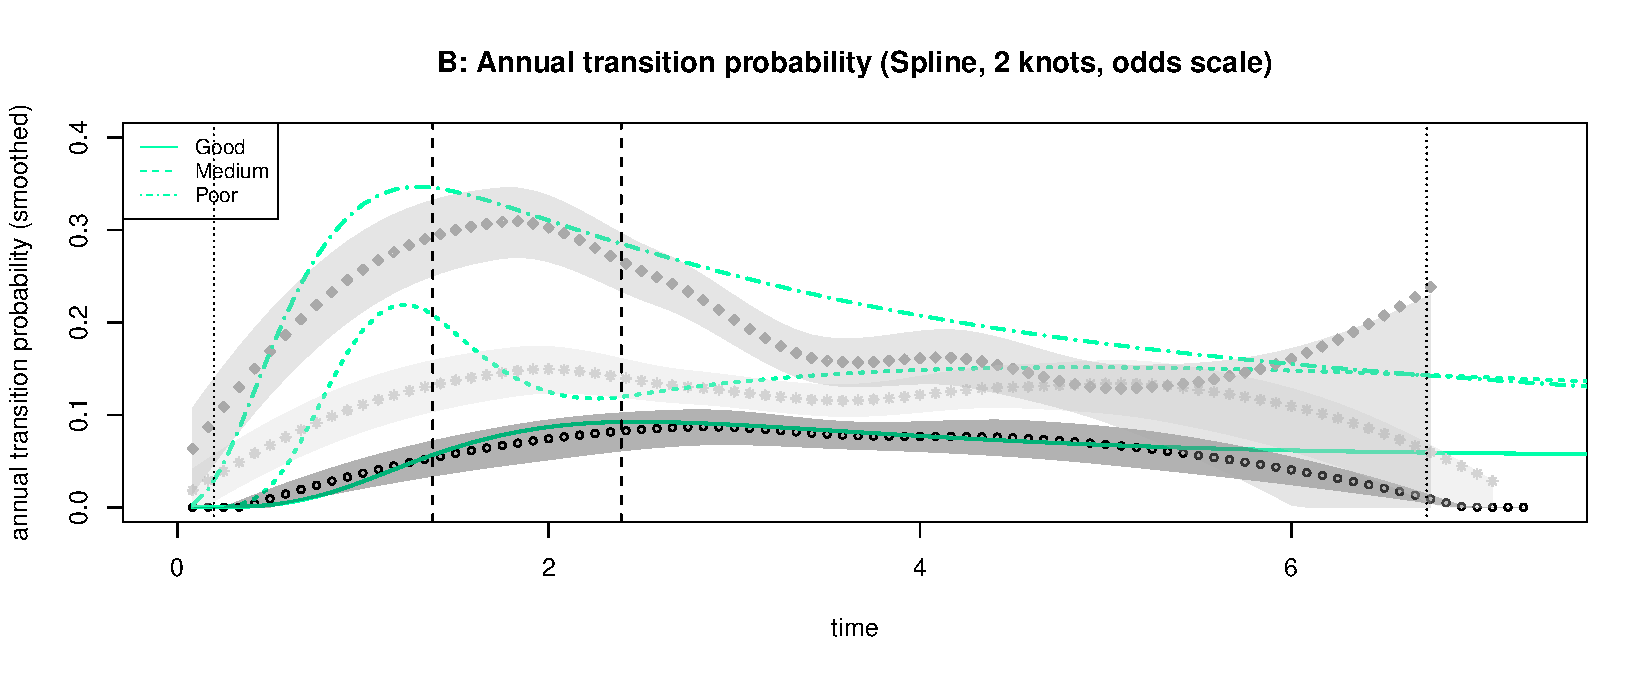
\includegraphics[height=0.3\textheight]{Images/spline_odds2-2} \end{flushleft}

\begin{flushleft}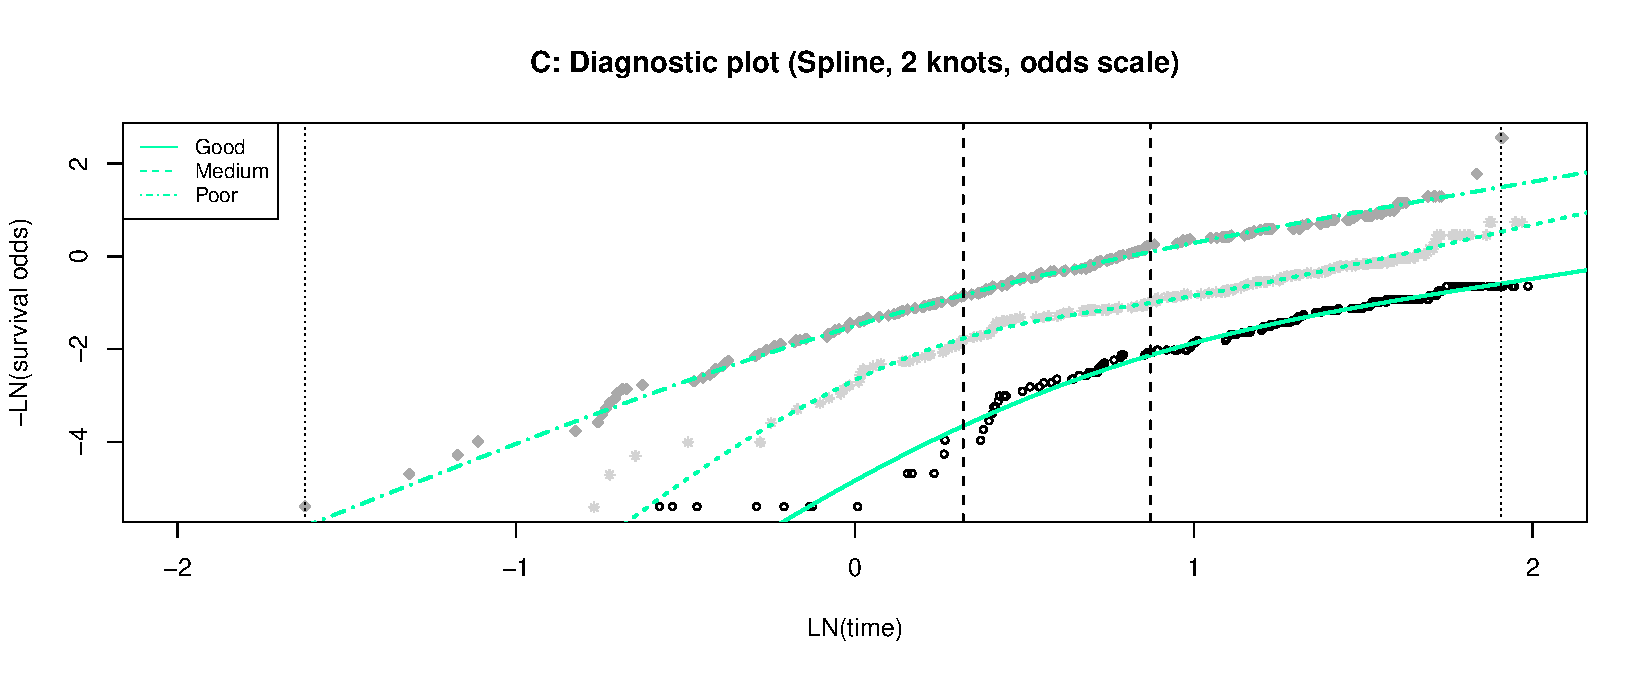
\includegraphics[height=0.3\textheight]{Images/spline_odds2-3} \end{flushleft}

\hypertarget{spline-odds-3-knots}{%
\subsection{Spline odds 3 knots}\label{spline-odds-3-knots}}

\begin{flushleft}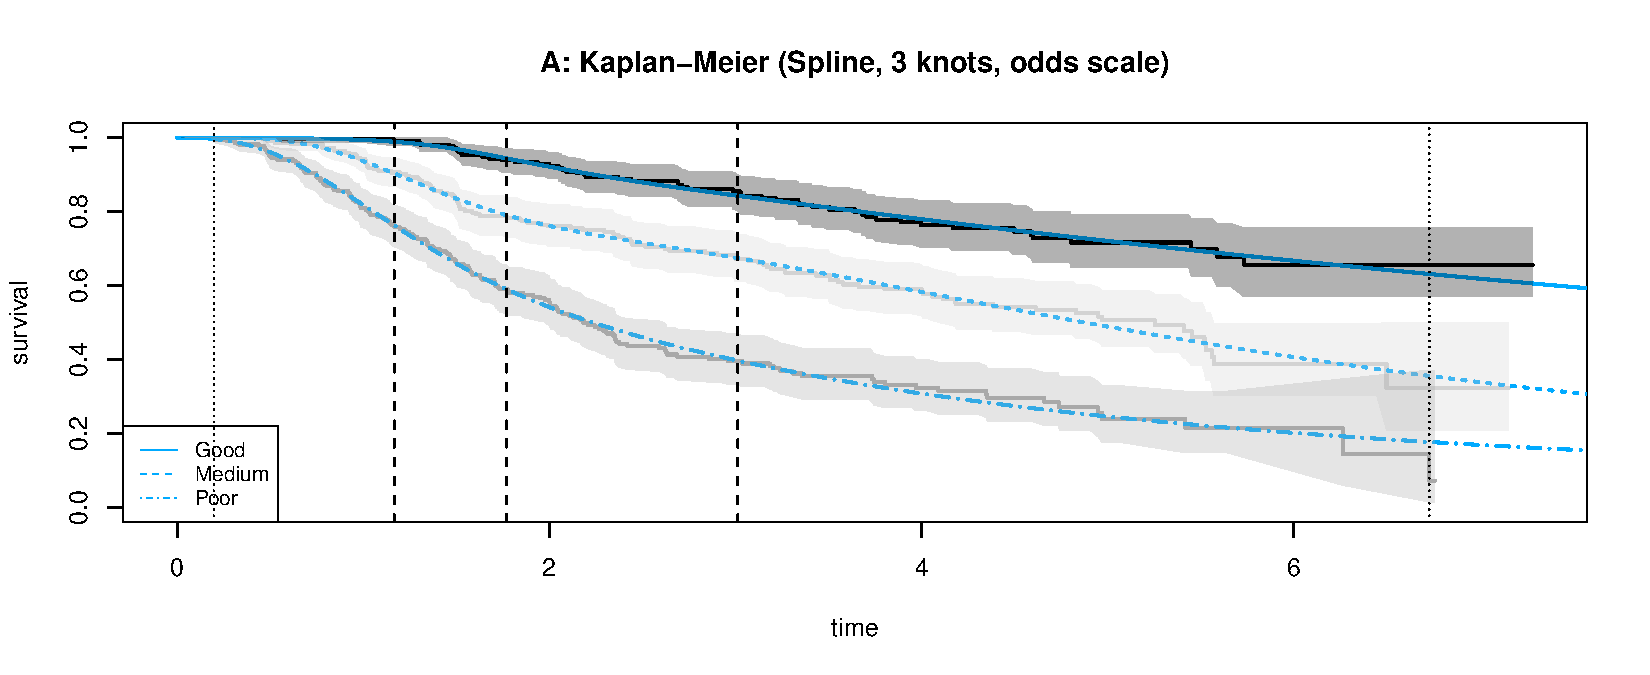
\includegraphics[height=0.3\textheight]{Images/spline_odds3-1} \end{flushleft}

\begin{flushleft}\includegraphics[height=0.3\textheight]{Images/spline_odds3-2} \end{flushleft}

\begin{flushleft}\includegraphics[height=0.3\textheight]{Images/spline_odds3-3} \end{flushleft}

\hypertarget{spline-normal-1-knot}{%
\subsection{Spline normal 1 knot}\label{spline-normal-1-knot}}

\begin{flushleft}\includegraphics[height=0.3\textheight]{Images/spline_norm1-1} \end{flushleft}

\begin{flushleft}\includegraphics[height=0.3\textheight]{Images/spline_norm1-2} \end{flushleft}

\begin{flushleft}\includegraphics[height=0.3\textheight]{Images/spline_norm1-3} \end{flushleft}

\hypertarget{spline-normal-2-knots}{%
\subsection{Spline normal 2 knots}\label{spline-normal-2-knots}}

\begin{flushleft}\includegraphics[height=0.3\textheight]{Images/spline_norm2-1} \end{flushleft}

\begin{flushleft}\includegraphics[height=0.3\textheight]{Images/spline_norm2-2} \end{flushleft}

\begin{flushleft}\includegraphics[height=0.3\textheight]{Images/spline_norm2-3} \end{flushleft}

\hypertarget{spline-normal-3-knots}{%
\subsection{Spline normal 3 knots}\label{spline-normal-3-knots}}

\begin{flushleft}\includegraphics[height=0.3\textheight]{Images/spline_norm3-1} \end{flushleft}

\begin{flushleft}\includegraphics[height=0.3\textheight]{Images/spline_norm3-2} \end{flushleft}

\begin{flushleft}\includegraphics[height=0.3\textheight]{Images/spline_norm3-3} \end{flushleft}

\newpage

\hypertarget{plausibility-of-the-long-term-extrapolation}{%
\section{Plausibility of the long-term
extrapolation}\label{plausibility-of-the-long-term-extrapolation}}

\hypertarget{which-models-isare-more-appropriate-for-long-term-extrapolation}{%
\subsection{Which model(s) is/are more appropriate for long-term
extrapolation?}\label{which-models-isare-more-appropriate-for-long-term-extrapolation}}

\hypertarget{areis-the-selected-models-plausible-in-comparison-with-general-population-mortality}{%
\subsection{Are/is the selected model(s) plausible in comparison with
general population
mortality?}\label{areis-the-selected-models-plausible-in-comparison-with-general-population-mortality}}

In this section, we present the estimated survival probabilities by
through fitted parametric survival models for the period of time within
and beyond data collection, i.e.~the extrapolation. This is done by 1)
plotting the survival curves (Figures A and B), 2) displaying the
survival probabilities at multiple time points (first Table), 3) ploting
conditional annual transition probabilities (Figures C and D), and
providing the summary statistics of the estimated conditional transition
probabilities (second Table). This information is provided for each
group separately.\\
One way to assess the plausibility of the extrapolated survival
probabilities is to compare the estimated survival probabilities at
different time points with external data (e.g.~observational data), and/
or to ask clinical experts about the plausibility of these
extrapolations. Another way to check for plausibility is to compare the
conditional transition probability with general population mortality
rates (these can be obtained through national statistics). Parametric
survival models providing conditional transition probabilities which are
lower than the general population mortality rates may not be suitable
because this would mean patients may have a lower probability of death
than the general population values. Such finding require either to
select an alternative model or to adjust the selected model for general
population mortality rates.\\
\textbf{Interpretation in this case}: The conditional annual
probabilities estimated by the two-knots spline-based model on the
hazard scale was most consistent with general population mortality data
of the Netherlands (although it might still require adjustment).
Ideally, one would validate the plausibility of the long-term
extrapolations of the two-knots spline-based model against external
data.

\hypertarget{group-good}{%
\subsection{Group Good}\label{group-good}}

\begin{flushleft}\includegraphics[height=0.29\textheight]{Images/validate_extrapolation1-1} \end{flushleft}

\begin{flushleft}\includegraphics[height=0.29\textheight]{Images/validate_extrapolation1-2} \end{flushleft}

\resizebox{\linewidth}{!}{
\begin{tabular}{lrrrrrrrrrrrr}
\toprule
  & T= 0 & T= 1 & T= 2 & T= 3 & T= 4 & T= 5 & T= 10 & T= 15 & T= 20 & T= 25 & T= 30 & T= 35\\
\midrule
\cellcolor{gray!6}{1. Exponential} & \cellcolor{gray!6}{1} & \cellcolor{gray!6}{0.941} & \cellcolor{gray!6}{0.886} & \cellcolor{gray!6}{0.834} & \cellcolor{gray!6}{0.785} & \cellcolor{gray!6}{0.739} & \cellcolor{gray!6}{0.547} & \cellcolor{gray!6}{0.404} & \cellcolor{gray!6}{0.299} & \cellcolor{gray!6}{0.221} & \cellcolor{gray!6}{0.163} & \cellcolor{gray!6}{0.121}\\
2. Weibull & 1 & 0.978 & 0.932 & 0.870 & 0.797 & 0.719 & 0.345 & 0.122 & 0.033 & 0.007 & 0.001 & 0.000\\
\cellcolor{gray!6}{3. Gompertz} & \cellcolor{gray!6}{1} & \cellcolor{gray!6}{0.962} & \cellcolor{gray!6}{0.917} & \cellcolor{gray!6}{0.863} & \cellcolor{gray!6}{0.801} & \cellcolor{gray!6}{0.729} & \cellcolor{gray!6}{0.280} & \cellcolor{gray!6}{0.015} & \cellcolor{gray!6}{0.000} & \cellcolor{gray!6}{0.000} & \cellcolor{gray!6}{0.000} & \cellcolor{gray!6}{0.000}\\
4. Log-normal & 1 & 0.986 & 0.933 & 0.861 & 0.785 & 0.713 & 0.441 & 0.287 & 0.196 & 0.139 & 0.102 & 0.076\\
\cellcolor{gray!6}{5. Log-logistic} & \cellcolor{gray!6}{1} & \cellcolor{gray!6}{0.980} & \cellcolor{gray!6}{0.932} & \cellcolor{gray!6}{0.865} & \cellcolor{gray!6}{0.789} & \cellcolor{gray!6}{0.712} & \cellcolor{gray!6}{0.403} & \cellcolor{gray!6}{0.240} & \cellcolor{gray!6}{0.156} & \cellcolor{gray!6}{0.108} & \cellcolor{gray!6}{0.080} & \cellcolor{gray!6}{0.061}\\
6. Gamma & 1 & 0.982 & 0.935 & 0.869 & 0.793 & 0.714 & 0.367 & 0.165 & 0.069 & 0.027 & 0.011 & 0.004\\
\cellcolor{gray!6}{7. Generalised Gamma} & \cellcolor{gray!6}{1} & \cellcolor{gray!6}{0.991} & \cellcolor{gray!6}{0.928} & \cellcolor{gray!6}{0.849} & \cellcolor{gray!6}{0.778} & \cellcolor{gray!6}{0.717} & \cellcolor{gray!6}{0.526} & \cellcolor{gray!6}{0.425} & \cellcolor{gray!6}{0.362} & \cellcolor{gray!6}{0.319} & \cellcolor{gray!6}{0.286} & \cellcolor{gray!6}{0.261}\\
8. Spline 1 knot hazard & 1 & 0.992 & 0.927 & 0.843 & 0.774 & 0.719 & 0.521 & 0.381 & 0.279 & 0.205 & 0.151 & 0.111\\
\cellcolor{gray!6}{9. Spline 2 knots hazard} & \cellcolor{gray!6}{1} & \cellcolor{gray!6}{0.992} & \cellcolor{gray!6}{0.928} & \cellcolor{gray!6}{0.843} & \cellcolor{gray!6}{0.774} & \cellcolor{gray!6}{0.719} & \cellcolor{gray!6}{0.523} & \cellcolor{gray!6}{0.384} & \cellcolor{gray!6}{0.283} & \cellcolor{gray!6}{0.210} & \cellcolor{gray!6}{0.156} & \cellcolor{gray!6}{0.116}\\
10. Spline 3 knots hazard & 1 & 0.994 & 0.922 & 0.843 & 0.779 & 0.721 & 0.486 & 0.319 & 0.205 & 0.130 & 0.081 & 0.050\\
\cellcolor{gray!6}{11. Spline 1 knot odds} & \cellcolor{gray!6}{1} & \cellcolor{gray!6}{0.992} & \cellcolor{gray!6}{0.927} & \cellcolor{gray!6}{0.843} & \cellcolor{gray!6}{0.774} & \cellcolor{gray!6}{0.718} & \cellcolor{gray!6}{0.532} & \cellcolor{gray!6}{0.415} & \cellcolor{gray!6}{0.338} & \cellcolor{gray!6}{0.283} & \cellcolor{gray!6}{0.242} & \cellcolor{gray!6}{0.211}\\
12. Spline 2 knots odds & 1 & 0.992 & 0.928 & 0.843 & 0.774 & 0.718 & 0.533 & 0.418 & 0.340 & 0.285 & 0.245 & 0.213\\
\cellcolor{gray!6}{13. Spline 3 knots odds} & \cellcolor{gray!6}{1} & \cellcolor{gray!6}{0.994} & \cellcolor{gray!6}{0.922} & \cellcolor{gray!6}{0.844} & \cellcolor{gray!6}{0.780} & \cellcolor{gray!6}{0.721} & \cellcolor{gray!6}{0.498} & \cellcolor{gray!6}{0.363} & \cellcolor{gray!6}{0.277} & \cellcolor{gray!6}{0.220} & \cellcolor{gray!6}{0.180} & \cellcolor{gray!6}{0.151}\\
14. Spline 1 knot normal & 1 & 0.992 & 0.926 & 0.847 & 0.778 & 0.719 & 0.515 & 0.391 & 0.308 & 0.250 & 0.207 & 0.174\\
\cellcolor{gray!6}{15. Spline 2 knots normal} & \cellcolor{gray!6}{1} & \cellcolor{gray!6}{0.992} & \cellcolor{gray!6}{0.929} & \cellcolor{gray!6}{0.842} & \cellcolor{gray!6}{0.773} & \cellcolor{gray!6}{0.718} & \cellcolor{gray!6}{0.538} & \cellcolor{gray!6}{0.426} & \cellcolor{gray!6}{0.350} & \cellcolor{gray!6}{0.295} & \cellcolor{gray!6}{0.253} & \cellcolor{gray!6}{0.220}\\
16. Spline 3 knots normal & 1 & 0.994 & 0.921 & 0.845 & 0.780 & 0.721 & 0.503 & 0.371 & 0.285 & 0.225 & 0.182 & 0.150\\
\bottomrule
\end{tabular}}

\begin{flushleft}\includegraphics[height=0.29\textheight]{Images/validate_extrapolation1-3} \end{flushleft}

\begin{flushleft}\includegraphics[height=0.29\textheight]{Images/validate_extrapolation1-4} \end{flushleft}

\begin{tabular}{lrrrrr}
\toprule
  & Min & Q1 & Median & Q3 & Max\\
\midrule
\cellcolor{gray!6}{1. Exponential} & \cellcolor{gray!6}{0.0585969} & \cellcolor{gray!6}{0.0585969} & \cellcolor{gray!6}{0.0585969} & \cellcolor{gray!6}{0.0585969} & \cellcolor{gray!6}{0.0585969}\\
10. Spline 3 knots hazard & 0.0003310 & 0.0798260 & 0.0865334 & 0.0909988 & 0.0996328\\
\cellcolor{gray!6}{2. Weibull} & \cellcolor{gray!6}{0.0039603} & \cellcolor{gray!6}{0.1641779} & \cellcolor{gray!6}{0.2507544} & \cellcolor{gray!6}{0.3170901} & \cellcolor{gray!6}{0.3714738}\\
3. Gompertz & 0.0342601 & 0.1256322 & 0.4037134 & 0.8634656 & 1.0000000\\
\cellcolor{gray!6}{4. Log-normal} & \cellcolor{gray!6}{0.0000121} & \cellcolor{gray!6}{0.0563972} & \cellcolor{gray!6}{0.0670524} & \cellcolor{gray!6}{0.0819079} & \cellcolor{gray!6}{0.0936091}\\
5. Log-logistic & 0.0022936 & 0.0533146 & 0.0700441 & 0.0935993 & 0.1092616\\
\cellcolor{gray!6}{6. Gamma} & \cellcolor{gray!6}{0.0014181} & \cellcolor{gray!6}{0.1390361} & \cellcolor{gray!6}{0.1644882} & \cellcolor{gray!6}{0.1750195} & \cellcolor{gray!6}{0.1807519}\\
7. Generalised Gamma & 0.0000000 & 0.0191123 & 0.0269247 & 0.0452063 & 0.0862100\\
\cellcolor{gray!6}{8. Spline 1 knot hazard} & \cellcolor{gray!6}{0.0000002} & \cellcolor{gray!6}{0.0592140} & \cellcolor{gray!6}{0.0598953} & \cellcolor{gray!6}{0.0610195} & \cellcolor{gray!6}{0.0916043}\\
9. Spline 2 knots hazard & 0.0000002 & 0.0576502 & 0.0585313 & 0.0599923 & 0.0923962\\
\cellcolor{gray!6}{11. Spline 1 knot odds} & \cellcolor{gray!6}{0.0000002} & \cellcolor{gray!6}{0.0281269} & \cellcolor{gray!6}{0.0363823} & \cellcolor{gray!6}{0.0502992} & \cellcolor{gray!6}{0.0917044}\\
12. Spline 2 knots odds & 0.0000002 & 0.0278516 & 0.0359503 & 0.0497462 & 0.0924439\\
\cellcolor{gray!6}{13. Spline 3 knots odds} & \cellcolor{gray!6}{0.0003253} & \cellcolor{gray!6}{0.0358147} & \cellcolor{gray!6}{0.0466608} & \cellcolor{gray!6}{0.0638606} & \cellcolor{gray!6}{0.0999099}\\
14. Spline 1 knot normal & 0.0000000 & 0.0345970 & 0.0424046 & 0.0560095 & 0.0865141\\
\cellcolor{gray!6}{15. Spline 2 knots normal} & \cellcolor{gray!6}{0.0000006} & \cellcolor{gray!6}{0.0281480} & \cellcolor{gray!6}{0.0348987} & \cellcolor{gray!6}{0.0473455} & \cellcolor{gray!6}{0.0953359}\\
16. Spline 3 knots normal & 0.0007793 & 0.0386308 & 0.0470013 & 0.0611992 & 0.0975846\\
\bottomrule
\end{tabular}

\begin{flushleft}\includegraphics[height=0.29\textheight]{Images/validate_extrapolation1-5} \end{flushleft}

\begin{flushleft}\includegraphics[height=0.29\textheight]{Images/validate_extrapolation1-6} \end{flushleft}

\newpage

\hypertarget{group-medium}{%
\subsection{Group Medium}\label{group-medium}}

\begin{flushleft}\includegraphics[height=0.29\textheight]{Images/validate_extrapolation2-1} \end{flushleft}

\begin{flushleft}\includegraphics[height=0.29\textheight]{Images/validate_extrapolation2-2} \end{flushleft}

\resizebox{\linewidth}{!}{
\begin{tabular}{lrrrrrrrrrrrr}
\toprule
  & T= 0 & T= 1 & T= 2 & T= 3 & T= 4 & T= 5 & T= 10 & T= 15 & T= 20 & T= 25 & T= 30 & T= 35\\
\midrule
\cellcolor{gray!6}{1. Exponential} & \cellcolor{gray!6}{1} & \cellcolor{gray!6}{0.872} & \cellcolor{gray!6}{0.761} & \cellcolor{gray!6}{0.663} & \cellcolor{gray!6}{0.578} & \cellcolor{gray!6}{0.505} & \cellcolor{gray!6}{0.255} & \cellcolor{gray!6}{0.128} & \cellcolor{gray!6}{0.065} & \cellcolor{gray!6}{0.033} & \cellcolor{gray!6}{0.016} & \cellcolor{gray!6}{0.008}\\
2. Weibull & 1 & 0.923 & 0.811 & 0.693 & 0.578 & 0.474 & 0.141 & 0.032 & 0.006 & 0.001 & 0.000 & 0.000\\
\cellcolor{gray!6}{3. Gompertz} & \cellcolor{gray!6}{1} & \cellcolor{gray!6}{0.898} & \cellcolor{gray!6}{0.794} & \cellcolor{gray!6}{0.689} & \cellcolor{gray!6}{0.586} & \cellcolor{gray!6}{0.486} & \cellcolor{gray!6}{0.117} & \cellcolor{gray!6}{0.007} & \cellcolor{gray!6}{0.000} & \cellcolor{gray!6}{0.000} & \cellcolor{gray!6}{0.000} & \cellcolor{gray!6}{0.000}\\
4. Log-normal & 1 & 0.935 & 0.797 & 0.668 & 0.560 & 0.473 & 0.228 & 0.126 & 0.077 & 0.050 & 0.034 & 0.024\\
\cellcolor{gray!6}{5. Log-logistic} & \cellcolor{gray!6}{1} & \cellcolor{gray!6}{0.927} & \cellcolor{gray!6}{0.801} & \cellcolor{gray!6}{0.673} & \cellcolor{gray!6}{0.561} & \cellcolor{gray!6}{0.468} & \cellcolor{gray!6}{0.218} & \cellcolor{gray!6}{0.124} & \cellcolor{gray!6}{0.081} & \cellcolor{gray!6}{0.057} & \cellcolor{gray!6}{0.043} & \cellcolor{gray!6}{0.034}\\
6. Gamma & 1 & 0.930 & 0.813 & 0.689 & 0.572 & 0.469 & 0.154 & 0.045 & 0.013 & 0.003 & 0.001 & 0.000\\
\cellcolor{gray!6}{7. Generalised Gamma} & \cellcolor{gray!6}{1} & \cellcolor{gray!6}{0.937} & \cellcolor{gray!6}{0.774} & \cellcolor{gray!6}{0.648} & \cellcolor{gray!6}{0.556} & \cellcolor{gray!6}{0.488} & \cellcolor{gray!6}{0.310} & \cellcolor{gray!6}{0.232} & \cellcolor{gray!6}{0.187} & \cellcolor{gray!6}{0.158} & \cellcolor{gray!6}{0.138} & \cellcolor{gray!6}{0.122}\\
8. Spline 1 knot hazard & 1 & 0.939 & 0.782 & 0.652 & 0.558 & 0.486 & 0.265 & 0.150 & 0.087 & 0.052 & 0.031 & 0.019\\
\cellcolor{gray!6}{9. Spline 2 knots hazard} & \cellcolor{gray!6}{1} & \cellcolor{gray!6}{0.935} & \cellcolor{gray!6}{0.766} & \cellcolor{gray!6}{0.673} & \cellcolor{gray!6}{0.579} & \cellcolor{gray!6}{0.490} & \cellcolor{gray!6}{0.184} & \cellcolor{gray!6}{0.061} & \cellcolor{gray!6}{0.018} & \cellcolor{gray!6}{0.005} & \cellcolor{gray!6}{0.001} & \cellcolor{gray!6}{0.000}\\
10. Spline 3 knots hazard & 1 & 0.936 & 0.761 & 0.674 & 0.585 & 0.491 & 0.159 & 0.040 & 0.008 & 0.001 & 0.000 & 0.000\\
\cellcolor{gray!6}{11. Spline 1 knot odds} & \cellcolor{gray!6}{1} & \cellcolor{gray!6}{0.939} & \cellcolor{gray!6}{0.778} & \cellcolor{gray!6}{0.648} & \cellcolor{gray!6}{0.556} & \cellcolor{gray!6}{0.489} & \cellcolor{gray!6}{0.301} & \cellcolor{gray!6}{0.213} & \cellcolor{gray!6}{0.162} & \cellcolor{gray!6}{0.131} & \cellcolor{gray!6}{0.109} & \cellcolor{gray!6}{0.093}\\
12. Spline 2 knots odds & 1 & 0.935 & 0.769 & 0.673 & 0.576 & 0.489 & 0.235 & 0.136 & 0.089 & 0.063 & 0.048 & 0.037\\
\cellcolor{gray!6}{13. Spline 3 knots odds} & \cellcolor{gray!6}{1} & \cellcolor{gray!6}{0.937} & \cellcolor{gray!6}{0.761} & \cellcolor{gray!6}{0.675} & \cellcolor{gray!6}{0.583} & \cellcolor{gray!6}{0.489} & \cellcolor{gray!6}{0.207} & \cellcolor{gray!6}{0.108} & \cellcolor{gray!6}{0.066} & \cellcolor{gray!6}{0.044} & \cellcolor{gray!6}{0.032} & \cellcolor{gray!6}{0.024}\\
14. Spline 1 knot normal & 1 & 0.938 & 0.775 & 0.648 & 0.557 & 0.488 & 0.290 & 0.195 & 0.141 & 0.107 & 0.084 & 0.067\\
\cellcolor{gray!6}{15. Spline 2 knots normal} & \cellcolor{gray!6}{1} & \cellcolor{gray!6}{0.930} & \cellcolor{gray!6}{0.773} & \cellcolor{gray!6}{0.669} & \cellcolor{gray!6}{0.572} & \cellcolor{gray!6}{0.489} & \cellcolor{gray!6}{0.240} & \cellcolor{gray!6}{0.135} & \cellcolor{gray!6}{0.083} & \cellcolor{gray!6}{0.054} & \cellcolor{gray!6}{0.037} & \cellcolor{gray!6}{0.026}\\
16. Spline 3 knots normal & 1 & 0.937 & 0.761 & 0.675 & 0.583 & 0.489 & 0.198 & 0.091 & 0.047 & 0.026 & 0.015 & 0.010\\
\bottomrule
\end{tabular}}

\begin{flushleft}\includegraphics[height=0.29\textheight]{Images/validate_extrapolation2-3} \end{flushleft}

\begin{flushleft}\includegraphics[height=0.29\textheight]{Images/validate_extrapolation2-4} \end{flushleft}

\begin{tabular}{lrrrrr}
\toprule
  & Min & Q1 & Median & Q3 & Max\\
\midrule
\cellcolor{gray!6}{1. Exponential} & \cellcolor{gray!6}{0.1278820} & \cellcolor{gray!6}{0.1278820} & \cellcolor{gray!6}{0.1278820} & \cellcolor{gray!6}{0.1278820} & \cellcolor{gray!6}{0.1278820}\\
10. Spline 3 knots hazard & 0.0000040 & 0.2243467 & 0.2816554 & 0.3202621 & 0.3498686\\
\cellcolor{gray!6}{2. Weibull} & \cellcolor{gray!6}{0.0298491} & \cellcolor{gray!6}{0.2382194} & \cellcolor{gray!6}{0.2998675} & \cellcolor{gray!6}{0.3413164} & \cellcolor{gray!6}{0.3730304}\\
3. Gompertz & 0.0960264 & 0.2326209 & 0.5026105 & 0.8415103 & 1.0000000\\
\cellcolor{gray!6}{4. Log-normal} & \cellcolor{gray!6}{0.0004751} & \cellcolor{gray!6}{0.0692201} & \cellcolor{gray!6}{0.0864990} & \cellcolor{gray!6}{0.1175437} & \cellcolor{gray!6}{0.1630482}\\
5. Log-logistic & 0.0150627 & 0.0512119 & 0.0722192 & 0.1148301 & 0.1673124\\
\cellcolor{gray!6}{6. Gamma} & \cellcolor{gray!6}{0.0159374} & \cellcolor{gray!6}{0.2105278} & \cellcolor{gray!6}{0.2273428} & \cellcolor{gray!6}{0.2338793} & \cellcolor{gray!6}{0.2373538}\\
7. Generalised Gamma & 0.0000000 & 0.0249765 & 0.0361491 & 0.0643696 & 0.1783037\\
\cellcolor{gray!6}{8. Spline 1 knot hazard} & \cellcolor{gray!6}{0.0005533} & \cellcolor{gray!6}{0.0961200} & \cellcolor{gray!6}{0.1007177} & \cellcolor{gray!6}{0.1087714} & \cellcolor{gray!6}{0.1767370}\\
9. Spline 2 knots hazard & 0.0000006 & 0.1921569 & 0.2213494 & 0.2415978 & 0.2568265\\
\cellcolor{gray!6}{11. Spline 1 knot odds} & \cellcolor{gray!6}{0.0004610} & \cellcolor{gray!6}{0.0331955} & \cellcolor{gray!6}{0.0461415} & \cellcolor{gray!6}{0.0743721} & \cellcolor{gray!6}{0.1809477}\\
12. Spline 2 knots odds & 0.0000004 & 0.0500917 & 0.0706148 & 0.1135216 & 0.2192447\\
\cellcolor{gray!6}{13. Spline 3 knots odds} & \cellcolor{gray!6}{0.0000052} & \cellcolor{gray!6}{0.0581364} & \cellcolor{gray!6}{0.0821832} & \cellcolor{gray!6}{0.1255993} & \cellcolor{gray!6}{0.2117141}\\
14. Spline 1 knot normal & 0.0000012 & 0.0444894 & 0.0569700 & 0.0823605 & 0.1804334\\
\cellcolor{gray!6}{15. Spline 2 knots normal} & \cellcolor{gray!6}{0.0000000} & \cellcolor{gray!6}{0.0682231} & \cellcolor{gray!6}{0.0852159} & \cellcolor{gray!6}{0.1164045} & \cellcolor{gray!6}{0.2005479}\\
16. Spline 3 knots normal & 0.0000001 & 0.0939627 & 0.1132858 & 0.1426801 & 0.2122248\\
\bottomrule
\end{tabular}

\begin{flushleft}\includegraphics[height=0.29\textheight]{Images/validate_extrapolation2-5} \end{flushleft}

\begin{flushleft}\includegraphics[height=0.29\textheight]{Images/validate_extrapolation2-6} \end{flushleft}

\newpage

\hypertarget{group-poor}{%
\subsection{Group Poor}\label{group-poor}}

\begin{flushleft}\includegraphics[height=0.29\textheight]{Images/validate_extrapolation3-1} \end{flushleft}

\begin{flushleft}\includegraphics[height=0.29\textheight]{Images/validate_extrapolation3-2} \end{flushleft}

\resizebox{\linewidth}{!}{
\begin{tabular}{lrrrrrrrrrrrr}
\toprule
  & T= 0 & T= 1 & T= 2 & T= 3 & T= 4 & T= 5 & T= 10 & T= 15 & T= 20 & T= 25 & T= 30 & T= 35\\
\midrule
\cellcolor{gray!6}{1. Exponential} & \cellcolor{gray!6}{1} & \cellcolor{gray!6}{0.755} & \cellcolor{gray!6}{0.570} & \cellcolor{gray!6}{0.430} & \cellcolor{gray!6}{0.325} & \cellcolor{gray!6}{0.245} & \cellcolor{gray!6}{0.060} & \cellcolor{gray!6}{0.015} & \cellcolor{gray!6}{0.004} & \cellcolor{gray!6}{0.001} & \cellcolor{gray!6}{0.000} & \cellcolor{gray!6}{0.000}\\
2. Weibull & 1 & 0.817 & 0.608 & 0.430 & 0.292 & 0.193 & 0.017 & 0.001 & 0.000 & 0.000 & 0.000 & 0.000\\
\cellcolor{gray!6}{3. Gompertz} & \cellcolor{gray!6}{1} & \cellcolor{gray!6}{0.776} & \cellcolor{gray!6}{0.588} & \cellcolor{gray!6}{0.436} & \cellcolor{gray!6}{0.315} & \cellcolor{gray!6}{0.221} & \cellcolor{gray!6}{0.022} & \cellcolor{gray!6}{0.001} & \cellcolor{gray!6}{0.000} & \cellcolor{gray!6}{0.000} & \cellcolor{gray!6}{0.000} & \cellcolor{gray!6}{0.000}\\
4. Log-normal & 1 & 0.820 & 0.572 & 0.401 & 0.289 & 0.214 & 0.063 & 0.025 & 0.012 & 0.006 & 0.004 & 0.002\\
\cellcolor{gray!6}{5. Log-logistic} & \cellcolor{gray!6}{1} & \cellcolor{gray!6}{0.819} & \cellcolor{gray!6}{0.568} & \cellcolor{gray!6}{0.389} & \cellcolor{gray!6}{0.275} & \cellcolor{gray!6}{0.203} & \cellcolor{gray!6}{0.069} & \cellcolor{gray!6}{0.034} & \cellcolor{gray!6}{0.021} & \cellcolor{gray!6}{0.014} & \cellcolor{gray!6}{0.010} & \cellcolor{gray!6}{0.008}\\
6. Gamma & 1 & 0.829 & 0.605 & 0.420 & 0.283 & 0.187 & 0.020 & 0.002 & 0.000 & 0.000 & 0.000 & 0.000\\
\cellcolor{gray!6}{7. Generalised Gamma} & \cellcolor{gray!6}{1} & \cellcolor{gray!6}{0.810} & \cellcolor{gray!6}{0.555} & \cellcolor{gray!6}{0.399} & \cellcolor{gray!6}{0.302} & \cellcolor{gray!6}{0.237} & \cellcolor{gray!6}{0.100} & \cellcolor{gray!6}{0.057} & \cellcolor{gray!6}{0.037} & \cellcolor{gray!6}{0.026} & \cellcolor{gray!6}{0.019} & \cellcolor{gray!6}{0.015}\\
8. Spline 1 knot hazard & 1 & 0.822 & 0.545 & 0.390 & 0.301 & 0.244 & 0.109 & 0.056 & 0.031 & 0.018 & 0.011 & 0.007\\
\cellcolor{gray!6}{9. Spline 2 knots hazard} & \cellcolor{gray!6}{1} & \cellcolor{gray!6}{0.817} & \cellcolor{gray!6}{0.546} & \cellcolor{gray!6}{0.396} & \cellcolor{gray!6}{0.305} & \cellcolor{gray!6}{0.243} & \cellcolor{gray!6}{0.096} & \cellcolor{gray!6}{0.043} & \cellcolor{gray!6}{0.021} & \cellcolor{gray!6}{0.010} & \cellcolor{gray!6}{0.005} & \cellcolor{gray!6}{0.003}\\
10. Spline 3 knots hazard & 1 & 0.819 & 0.540 & 0.400 & 0.310 & 0.243 & 0.081 & 0.030 & 0.012 & 0.005 & 0.002 & 0.001\\
\cellcolor{gray!6}{11. Spline 1 knot odds} & \cellcolor{gray!6}{1} & \cellcolor{gray!6}{0.820} & \cellcolor{gray!6}{0.542} & \cellcolor{gray!6}{0.390} & \cellcolor{gray!6}{0.303} & \cellcolor{gray!6}{0.248} & \cellcolor{gray!6}{0.127} & \cellcolor{gray!6}{0.082} & \cellcolor{gray!6}{0.060} & \cellcolor{gray!6}{0.047} & \cellcolor{gray!6}{0.038} & \cellcolor{gray!6}{0.032}\\
12. Spline 2 knots odds & 1 & 0.817 & 0.544 & 0.393 & 0.304 & 0.246 & 0.120 & 0.075 & 0.054 & 0.041 & 0.033 & 0.027\\
\cellcolor{gray!6}{13. Spline 3 knots odds} & \cellcolor{gray!6}{1} & \cellcolor{gray!6}{0.818} & \cellcolor{gray!6}{0.542} & \cellcolor{gray!6}{0.398} & \cellcolor{gray!6}{0.308} & \cellcolor{gray!6}{0.246} & \cellcolor{gray!6}{0.110} & \cellcolor{gray!6}{0.065} & \cellcolor{gray!6}{0.044} & \cellcolor{gray!6}{0.033} & \cellcolor{gray!6}{0.026} & \cellcolor{gray!6}{0.021}\\
14. Spline 1 knot normal & 1 & 0.811 & 0.549 & 0.398 & 0.305 & 0.242 & 0.102 & 0.054 & 0.033 & 0.021 & 0.015 & 0.011\\
\cellcolor{gray!6}{15. Spline 2 knots normal} & \cellcolor{gray!6}{1} & \cellcolor{gray!6}{0.815} & \cellcolor{gray!6}{0.546} & \cellcolor{gray!6}{0.392} & \cellcolor{gray!6}{0.303} & \cellcolor{gray!6}{0.245} & \cellcolor{gray!6}{0.113} & \cellcolor{gray!6}{0.065} & \cellcolor{gray!6}{0.042} & \cellcolor{gray!6}{0.029} & \cellcolor{gray!6}{0.021} & \cellcolor{gray!6}{0.016}\\
16. Spline 3 knots normal & 1 & 0.818 & 0.541 & 0.398 & 0.308 & 0.244 & 0.100 & 0.051 & 0.030 & 0.019 & 0.013 & 0.009\\
\bottomrule
\end{tabular}}

\begin{flushleft}\includegraphics[height=0.29\textheight]{Images/validate_extrapolation3-3} \end{flushleft}

\begin{flushleft}\includegraphics[height=0.29\textheight]{Images/validate_extrapolation3-4} \end{flushleft}

\begin{tabular}{lrrrrr}
\toprule
  & Min & Q1 & Median & Q3 & Max\\
\midrule
\cellcolor{gray!6}{1. Exponential} & \cellcolor{gray!6}{0.2449482} & \cellcolor{gray!6}{0.2449482} & \cellcolor{gray!6}{0.2449482} & \cellcolor{gray!6}{0.2449482} & \cellcolor{gray!6}{0.2449482}\\
10. Spline 3 knots hazard & 0.0031604 & 0.1581132 & 0.1681704 & 0.1865373 & 0.3590229\\
\cellcolor{gray!6}{2. Weibull} & \cellcolor{gray!6}{0.0907442} & \cellcolor{gray!6}{0.4105709} & \cellcolor{gray!6}{0.4790585} & \cellcolor{gray!6}{0.5216195} & \cellcolor{gray!6}{0.5525972}\\
3. Gompertz & 0.2169796 & 0.3698466 & 0.5818235 & 0.8071868 & 1.0000000\\
\cellcolor{gray!6}{4. Log-normal} & \cellcolor{gray!6}{0.0022958} & \cellcolor{gray!6}{0.1000774} & \cellcolor{gray!6}{0.1279068} & \cellcolor{gray!6}{0.1841659} & \cellcolor{gray!6}{0.3070152}\\
5. Log-logistic & 0.0305143 & 0.0571627 & 0.0832145 & 0.1494462 & 0.3207417\\
\cellcolor{gray!6}{6. Gamma} & \cellcolor{gray!6}{0.0471845} & \cellcolor{gray!6}{0.3701940} & \cellcolor{gray!6}{0.3852535} & \cellcolor{gray!6}{0.3907371} & \cellcolor{gray!6}{0.3935697}\\
7. Generalised Gamma & 0.0000317 & 0.0518395 & 0.0728961 & 0.1237607 & 0.3222943\\
\cellcolor{gray!6}{8. Spline 1 knot hazard} & \cellcolor{gray!6}{0.0048605} & \cellcolor{gray!6}{0.0929348} & \cellcolor{gray!6}{0.1060806} & \cellcolor{gray!6}{0.1322263} & \cellcolor{gray!6}{0.3462113}\\
9. Spline 2 knots hazard & 0.0027621 & 0.1183362 & 0.1309295 & 0.1552006 & 0.3471134\\
\cellcolor{gray!6}{11. Spline 1 knot odds} & \cellcolor{gray!6}{0.0040186} & \cellcolor{gray!6}{0.0370407} & \cellcolor{gray!6}{0.0534928} & \cellcolor{gray!6}{0.0956147} & \cellcolor{gray!6}{0.3493116}\\
12. Spline 2 knots odds & 0.0029239 & 0.0397013 & 0.0573770 & 0.1025038 & 0.3469030\\
\cellcolor{gray!6}{13. Spline 3 knots odds} & \cellcolor{gray!6}{0.0031346} & \cellcolor{gray!6}{0.0443526} & \cellcolor{gray!6}{0.0641665} & \cellcolor{gray!6}{0.1145082} & \cellcolor{gray!6}{0.3547245}\\
14. Spline 1 knot normal & 0.0001727 & 0.0667705 & 0.0870224 & 0.1315769 & 0.3327152\\
\cellcolor{gray!6}{15. Spline 2 knots normal} & \cellcolor{gray!6}{0.0003302} & \cellcolor{gray!6}{0.0575542} & \cellcolor{gray!6}{0.0758377} & \cellcolor{gray!6}{0.1164719} & \cellcolor{gray!6}{0.3361441}\\
16. Spline 3 knots normal & 0.0005575 & 0.0702242 & 0.0912163 & 0.1362709 & 0.3562720\\
\bottomrule
\end{tabular}

\begin{flushleft}\includegraphics[height=0.29\textheight]{Images/validate_extrapolation3-5} \end{flushleft}

\begin{flushleft}\includegraphics[height=0.29\textheight]{Images/validate_extrapolation3-6} \end{flushleft}

\newpage

\hypertarget{session-information}{%
\section{Session information}\label{session-information}}

\begin{verbatim}
## R version 4.0.3 (2020-10-10)
## Platform: x86_64-w64-mingw32/x64 (64-bit)
## Running under: Windows 10 x64 (build 17763)
## 
## Matrix products: default
## 
## Random number generation:
##  RNG:     Mersenne-Twister 
##  Normal:  Inversion 
##  Sample:  Rejection 
##  
## attached base packages:
## [1] splines   stats     graphics  grDevices utils     datasets  methods  
## [8] base     
## 
## other attached packages:
##  [1] sft_2.2-1          SuppDists_1.1-9.5  fda_5.1.9          fds_1.8           
##  [5] RCurl_1.98-1.2     rainbow_3.6        pcaPP_1.9-73       MASS_7.3-53       
##  [9] Matrix_1.2-18      kableExtra_1.3.1   knitr_1.31         summarytools_0.9.8
## [13] data.table_1.13.6  survminer_0.4.8    ggpubr_0.4.0       muhaz_1.2.6.1     
## [17] flexsurv_1.1.1     rms_6.1-0          SparseM_1.78       Hmisc_4.4-2       
## [21] ggplot2_3.3.3      Formula_1.2-4      survival_3.2-7     lattice_0.20-41   
## 
## loaded via a namespace (and not attached):
##   [1] TH.data_1.0-10      colorspace_2.0-0    ggsignif_0.6.0     
##   [4] pryr_0.1.4          ellipsis_0.3.1      rio_0.5.16         
##   [7] mclust_5.4.7        htmlTable_2.1.0     base64enc_0.1-3    
##  [10] rstudioapi_0.13     farver_2.0.3        MatrixModels_0.4-1 
##  [13] mvtnorm_1.1-1       lubridate_1.7.9.2   xml2_1.3.2         
##  [16] codetools_0.2-16    broom_0.7.3         km.ci_0.5-2        
##  [19] cluster_2.1.0       png_0.1-7           compiler_4.0.3     
##  [22] httr_1.4.2          backports_1.2.0     assertthat_0.2.1   
##  [25] htmltools_0.5.1.1   quantreg_5.83       tools_4.0.3        
##  [28] gtable_0.3.0        glue_1.4.2          dplyr_1.0.3        
##  [31] Rcpp_1.0.6          carData_3.0-4       cellranger_1.1.0   
##  [34] vctrs_0.3.6         nlme_3.1-149        conquer_1.0.2      
##  [37] xfun_0.20           stringr_1.4.0       openxlsx_4.2.3     
##  [40] rvest_0.3.6         lifecycle_0.2.0     rstatix_0.6.0      
##  [43] polspline_1.1.19    zoo_1.8-8           scales_1.1.1       
##  [46] hms_1.0.0           sandwich_3.0-0      RColorBrewer_1.1-2 
##  [49] yaml_2.2.1          curl_4.3            gridExtra_2.3      
##  [52] KMsurv_0.1-5        pander_0.6.3        rpart_4.1-15       
##  [55] latticeExtra_0.6-29 stringi_1.5.3       checkmate_2.0.0    
##  [58] zip_2.1.1           hdrcde_3.4          bitops_1.0-6       
##  [61] rlang_0.4.10        pkgconfig_2.0.3     matrixStats_0.57.0 
##  [64] evaluate_0.14       purrr_0.3.4         labeling_0.4.2     
##  [67] ks_1.12.0           rapportools_1.0     htmlwidgets_1.5.3  
##  [70] tidyselect_1.1.0    deSolve_1.28        plyr_1.8.6         
##  [73] magrittr_2.0.1      R6_2.5.0            magick_2.6.0       
##  [76] generics_0.1.0      multcomp_1.4-15     DBI_1.1.1          
##  [79] pillar_1.4.7        haven_2.3.1         foreign_0.8-80     
##  [82] withr_2.4.1         abind_1.4-5         nnet_7.3-14        
##  [85] tibble_3.0.5        mstate_0.3.1        crayon_1.3.4       
##  [88] car_3.0-10          survMisc_0.5.5      KernSmooth_2.23-17 
##  [91] rmarkdown_2.6       jpeg_0.1-8.1        grid_4.0.3         
##  [94] readxl_1.3.1        forcats_0.5.1       digest_0.6.27      
##  [97] webshot_0.5.2       xtable_1.8-4        tidyr_1.1.2        
## [100] munsell_0.5.0       viridisLite_0.3.0   tcltk_4.0.3        
## [103] quadprog_1.5-8
\end{verbatim}

\end{document}
